\chapter{Un modèle pour détecter les isotopies sexuelles}
% A intégrer ici :
% quittant pour de bon les problématiques grammaticales du chapitre précédent

L'un des objectifs de notre recherche est d'aider à l'identification de passages dont la sexualité est un outil discursif ou un thème dans les textes latins classiques et tardifs. Comme J.N. Adams, nous ne distinguerons pas dans notre recherche les usages de la sexualité comme moyens d'appuyer une problématique autre (cf. usage de \textit{mollus} comme outil de dévalorisation) d'un discours sur les pratiques d'un personnage (comme ceux sur Philaenis chez Martial). Nous nous intéresserons dans un premier temps à la définition, dans le cadre du traitement automatique des langues, de cette tâche d'identification en l'intégrant dans le faible réseau des recherches similaires dans le domaine littéraire. Nous présenterons ensuite les différentes architectures de données et de modèles que nous avons testés. Nous nous intéresserons ensuite aux résultats, à ĺ'interprétation des échecs de certains modèles, à l'extensibilité des modèles, mais aussi aux valeurs constamment apprises par l'ensemble des modèles. Enfin, nous utiliserons les modèles comme outils de prédiction dans le cadre d'une étude de terrain sur le \textit{Centon Nuptial} d'Ausone et l'Énéide de Virgile, nous aidant à comprendre l'intérêt du modèle pour la recherche "traditionnelle", ses limites et les possibles améliorations à prévoir.

\section{La détection thématique, les sciences de l'antiquité et l'apprentissage profond}

% Aggarwal and Zhai (2012) defined the text classification task as given the training set D = {X1, ..., Xn}, where each data point Xi ∈ D is labeled with a value derived from the set of labels are numbered {1. . . k}

\begin{quote}[\textit{Cento Nuptialis}, 115]{Ausone}
    \textit{huc iuvenis nota fertur regione \textbf{viarum}} \\
    \enquote{Là se porte le jeune chef, par des voies qu'il connaît}\footcite{ausone_d_2010}
\end{quote}

\begin{quote}[\textit{Épigrammes}, 2, 33, 4]{Martial}
    \textit{Haec qui basiat, o Philaeni, \textbf{fellat}. \\}
    \enquote{Qui embrasse ces choses, ô Philaenis, suce.}
\end{quote}

\begin{quote}[54]{\textit{Priapées}}
    \textit{\textbf{CD} si scribas temonemque insuper addas, qui medium uult te scindere , pictus erit.} \\
    \enquote{Si tu écris CD et que tu ajoutes en plus un timon, Il y aura dessiné ce qui veut te déchirer le milieu}
\end{quote}

\begin{quote}[\textit{Gynaeciorum Sorani}, 1, 21]{Caelius Aurelianus}
    \textit{Interior ergo pars collo \textbf{matricis} connectitur , exterius vero fibris adnexa est quas \textbf{pinnas} vocant \textbf{feminini sinus}} \\
    \enquote{Ainsi, la partie la plus à l'intérieure est connectée au col de la \textbf{matrice}, quant à l'extérieur, elle est rattachée aux plis que l'on appelle les \textbf{ailes} du \textbf{giron féminin}.}
\end{quote}

Ces quatre textes ne partagent aucun terme voire lexique en commun autre que des mots outils et pourtant tous partagent une chose: ils parlent de sexualité. Par des voix détournées (métaphore d'Ausone), par un lexique identifié (Martial), à travers un rébus et un langage figuré (Priapées) ou bien dans un discours médical (Caelius), chacun de ces textes en parle. Pour le premier, dans le contexte de la nuit de noces et de la chambre des mariés, l'actualisation de /mouvement/ de \textit{fertur} et de /chemin-empruntable/ de \textit{viarum} portent l'isotopie d'une pénétration débutante. De même, les sèmes d'/entrée/ et /diviser/ de \textit{scindere} et /centre/ de l'/humain/ pour \textit{medium te} émettent pour la Priapée 54 l'information suffisante pour comprendre une menace de \textit{fututio} ou de \textit{pedicatio}: l'auteur annonce vouloir élargir l'endroit pénétré avec violence. Enfin, pudiquement et via l'emprunt au grec, ce sont les sèmes /forme-élancée/ et /deux/ de \textit{pinnas} attachés aux /sillon/, /féminin/ et /producteur/ de \textit{sinus feminini}, représentant le vagin, qui évoquent les lèvres inférieures. Ces textes ont donc la particularité, via des actualisations diverses, de représenter des isotopies de la sexualité.

La détection isotopique\footnote{Par simplification, nous utiliserons aussi le terme de \textit{thématique}.} de la sexualité entre dans de multiples catégories de tâches du TAL. Ces tâches peuvent relever de problématiques purement commerciales, comme la classification automatique d'objets à vendre sur des \textit{market places}, mais sont aussi entrées dans le domaine des sciences de l'antiquité, et en particulier de l'étude des textes latins et grecs. Nous présenterons deux techniques de classification utilisées. Puis, nous nous intéresserons tour à tour à l'incursion du domaine computationnel dans le domaine de la philologie et de la littérature. Enfin, nous nous intéresserons aux tâches qui rejoignent la nôtre, soit par leurs méthodes, soit thématiquement.

\subsection{Entre classification de texte et analyse de similarité}

\subsubsection{Que classons-nous ?}


%En gros, ici:
%- quelle est l'unité que l'on cherche à détecter.
%- quelles sont les méthodes que l'on peut utiliser (classification vs. similarité)
% Faire aussi de la review rapide de littérature hors champs pour comparer

La détection isotopique revient à enseigner à une machine à reconnaître dans un échantillon de texte pré-séquencé $E$ l'existence d'un motif thématique $M$. Cette détection peut se relever facile dans quelques cas: la présence de termes d'un lexique spécifique, ici \textit{mentula}, \textit{futuo} ou \textit{cunnus}, ne laisse que peu de doute sur l'un des sèmes de l'échantillon. Cependant, elle devient beaucoup plus problématique pour la machine voire pour l'être humain lorsqu'un réseau d'abstraction, d'actualisations sémiques, permet de faire ressortir une isotopie, entre autres car \enquote{ce n'est pas la récurrence de sèmes déjà donnés qui constitue l'isotopie, mais, rétroactivement, la présomption d'isotopie qui permet d'actualiser des sèmes, voire les sèmes}\footcite[p. 34]{rastier_isotopie_1985}. Une approche d'apprentissage supervisé peut s'avérer intéressante: on apprend alors à la machine à passer de la présomption à la confirmation ou l'information de la présence d'isotopie.

Le développement de tels modèles pose un intérêt majeur pour les sciences humaines: il permettrait en effet de constituer rapidement des corpus thématiques. Ceux-ci donneraient à leur tour la capacité d'approfondir nos connaissances des modèles de pensées, anciens ou non, en forçant constamment cette présomption et en reposant sur d'autres biais que ceux des spécialistes. Un groupe de recherche pourrait alors, à partir de corpus d'exemples préparés à l'avance, commencer à entraîner un premier modèle, quitte à obtenir un haut taux d'erreurs, de corriger ces erreurs et d'agrandir ce corpus au fur et à mesure de ces corrections, dans un cercle vertueux apprentissage-annotation-correction. 

Ces modèles relèvent principalement de deux types d'architectures: une "classique", utilisant un apprentissage par étiquette (\textit{label} en anglais), et une plus récente et empruntée au domaine de la vision par ordinateur, qui s'effectue par mesure de similarité.

Les modèles de classification de textes par étiquette sont particulièrement ancrés dans le domaine du traitement automatique des langues. Il s'agit pour un modèle d'être entraîné à annoter une séquence de mots comme faisant partie d'une (classification simple) ou plusieurs catégories (classification \textit{multilabel}). Dans leur chapitre de 2012, C. Aggarwal et C.X. Zhai\footcite{aggarwal_survey_2012} la définissent comme l'entraînement d'un modèle visant à faire reconnaître dans un ensemble d'échantillons $D$ un nombre défini $k$ de catégories\footnote{Nous reprenons ici leurs signes.}. Ils réintroduisent la notion de classification douce (\textit{soft}) et dure (\textit{hard}): une épigramme de Martial serait ainsi attribuée à l'auteur Martial, tandis qu'elle pourrait être affiliée à l'isotopie de la sexualité et à celle des bains. Ils font aussi entrer la distinction entre une classification à probabilité -- un pourcentage est fourni pour chaque classe -- à une classification binaire où un seul label est fourni sans mesure: pour un texte de l'\textit{Anthologie Latine}, un texte pourrait ainsi soit présenter une probabilité d'être de Sénèque indépendamment de sa probabilité d'être de Virgile dans le cas du premier type de classification, tandis que le deuxième produirait une affirmation ou infirmation d'autorité.

Dans leur chapitre, C. Aggarwal et C. X. Zhai citent alors les modèles les plus communs en 2012, presque uniquement des modèles n'appartenant pas à la catégorie de l'apprentissage profond: classificateur bayésien, SVM, à base de règles ou d'arbres décisionnels. Ces modèles continuent d'être utilisés: ils représentent des solutions souvent peu coûteuses computationellement, efficaces dans de nombreux cas. Ces solutions ont par ailleurs la particularité de ne pas être nécessairement moins bonnes que les méthodes plus modernes, à apprentissage profond, dont le coût de calcul -- et donc énergétique -- est en général beaucoup plus grand\footcite{fell_comparing_2019}. Aujourd'hui, en \textit{deep learning}, ces modèles sont principalement représentés par des modèles dont la dernière couche est constituée de réseaux linéaires, bien qu'il existe une survivance pour cette couche des CRFs ou d'autres formes de couches de classification, notamment dans le cadre de classification au niveau mot\footcite{alkhwiter_part--speech_2021, shang_speaker-change_2020}.

% Les modèles de classification peuvent être utilisés à divers niveaux du texte, du document entier au mot, en passant par des séquences arbitraires produites par l'analyseur ou des séquences éditoriales. 
% Virer cette partie car reproduction de plus bas ?
% Parmi les classifications de texte, l'une des applications les plus connues dans le domaine des humanités est celle de l'analyse de sentiment, qui cherche à distinguer - au plus simple - des phrases positives ou négatives sur un sujet: R. Sprugnoli et ses collègues développaient ainsi en 2016 un outil pour étudier l'évolution de la perception de certains sujets dans un corpus historique\footcite{sprugnoli_towards_2016}. D'autres exemples de type de classification existent: des plus sensibles, tels que la détection d'appel à la haine ou d'apologie du terrorisme sur les réseaux sociaux, à des sujets au contraire beaucoup plus légers comme l'attribution d'auteur, de période d'écriture ou de dialecte. 

\begin{figure}
    \centering
    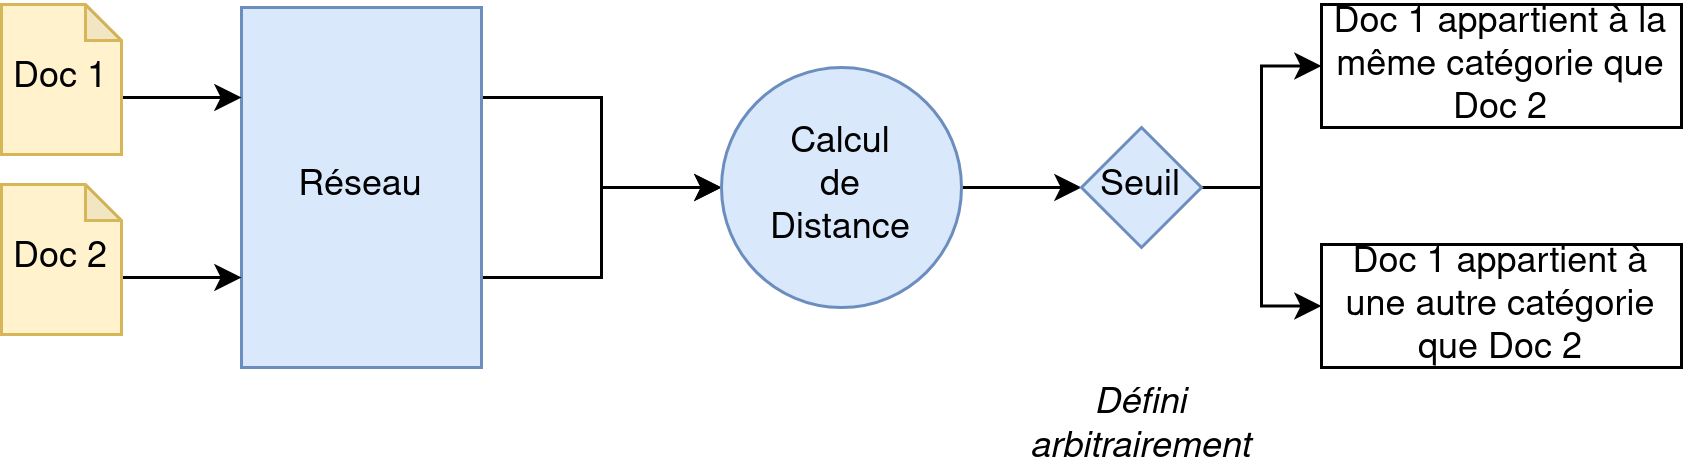
\includegraphics[width=\linewidth]{figures/chap4/Siamois.png}
    \caption{Architecture simplifiée d'un réseau siamois}
    \label{fig:chap4:structures:siamese-network}
\end{figure}

Malheureusement, les modèles de classification nécessitent en général un nombre conséquent de données d'entraînement pour être généralisables et donc dépasser le simple stade de preuve de concept. Si notre thématique est large et ses exemples répétés dans la littérature latine quelle que soit la période, l'objectif n'est pas ici de ne proposer une solution qu'à la question sexuelle: d'autres thématiques pourraient intéresser d'autres chercheurs (par exemple, la paternité, les phénomènes météorologiques en mer, etc.) et une étude des limites quantitatives s'impose. On peut aussi s'intéresser à un découpage de notre isotopie en plusieurs sous-ensembles, soit du point de vue de la stylistique -- usage métaphorique, explicite, comparatif, allusif --, des acteurs -- femmes, hommes, enfants, esclaves, etc. -- ou soit, encore, d'un point de vue moral -- condamnation, neutre, positif. Qu'il s'agisse d'un autre thème ou d'une section du nôtre, l'usage du cycle apprentissage-prédiction-correction comme outil de constitution de corpus dès la dizaine, la centaine ou le millier d'exemples change le temps de travail nécessaire à cette compilation. Or, pour ce qui est des architectures neuronales, la classification par étiquette est connue pour ses limites sur de petits corpus\footnote{Bien qu'il s'agisse d'un corpus d'images, on peut trouver une étude relativement bien fournie sur une comparaison entre ces deux types d'outils: \textcite{pasupa_comparison_2016}}. % Exemple ?

On s'intéresse alors à un autre mode de classification, celui par mesure de similarité et en particulier des modèles de réseaux siamois. Ces derniers incorporent la particularité de comparer au moins deux échantillons, dont l'un a une classe connue: après avoir produit une représentation numérique des échantillons, comme les modèles plus classiques, le réseau siamois est entraîné à réduire ou augmenter les distances entre ces échantillons afin de les catégoriser. À travers ces comparaisons, il va détecter plus rapidement les traits saillants des petites catégories. Cette architecture a le bénéfice d'être nettement plus efficace dans des situations dites de \textit{few-shot learning}, c'est-à-dire à faible set d'entraînement. 

Largement utilisé dans le domaine de la \textit{computer vision}, on en trouve un usage en histoire du livre à travers l'intéressant travail du projet Filigrane\footcite{shen_large-scale_2021} qui permet, dans des scores raisonnables, de classer facilement des filigranes papiers à partir de très peu d'exemples d'entraînement, mais y compris de potentiellement détecter des filigranes inconnus. Il est important de prendre en compte, lorsque l'on compare les scores des deux types d'architecture dans des publications différentes, la quantité des données d'entraînement: ces réseaux apprennent rapidement, pour des situations avec parfois de très nombreuses catégories. Dans un tel contexte, les modèles de classification ne proposent que rarement d'aussi bons résultats sans tomber dans le surapprentissage.

Avec un peu plus de deux mille exemples issus d'Adams, dans quel cas de figure se situe notre problème ? Si un tel set de données peut paraître important du point de vue d'un romaniste, il est en fait relativement bien faible comparé à des sets de données d'analyse de sentiment avec la pauvreté morphologique de l'anglais: assez petit, l'\textit{IMDB Movie Reviews Dataset}\footcite{maas-EtAl:2011:ACL-HLT2011}, un ensemble de critiques de films associées à des notes, ne compte \enquote{que} 50~000 exemples, à l'autre bout du spectre, l'\textit{Amazon Review Data}\footcite{ni_justifying_2019} en compte 233.1 millions. En regard de ces chiffres, notre modèle se limiterait-il à une recherche par similarité ? Rien n'est moins sûr, car, au contraire de l'exemple des filigranes, non seulement le nombre d'exemples pour une même catégorie est beaucoup plus élevé (les 2000 exemples relèvent de l'isotopie sexuelle), mais la variété à l'intérieur de ce set est beaucoup plus large: entre une métaphore militaire du courtisan d'Ithaque qui bande son arme et une claire mention d'\textit{irrumo}, la ressemblance est mince, tandis que deux prises de vue du même filigrane ont plus de points communs. C'est entre autres pourquoi nous nous appliquerons à évaluer la résistance des deux types d'architecture en fonction de plusieurs paramètres, y compris celui de la taille du set d'entraînement, dans l'optique de favoriser la construction \textit{ex nihilo} de futurs corpus sur d'autres thématiques.

% C'est une question importante, mais je me demande si ça arrive au bon endroit.

Question quelque peu laissée pour compte jusque-là, la question de l'unité syntaxique ou sémantique dans laquelle on souhaite identifier l'isotopie sexuelle reste assez centrale. On peut distinguer plusieurs niveaux allant de l'oeuvre à celui du mot. Le premier niveau, le niveau \textit{oeuvre}, pose un problème d'élasticité des tailles -- entre une épigramme de deux vers de Martial et un livre de Tite-Live un monde existe -- et d'utilité de l'outil: il n'est probablement pas intéressant de savoir si on parle de sexualité dans un livre d'historien romain, mais plutôt d'où se trouveraient de tels usages. Le deuxième niveau consisterait donc à détecter l'information au sein de petites séquences éditoriales comme des  \textit{paragraphes}, mais ils posent le problème de l'équivalence en poésie classique ou en théâtre: si une épigramme ou un court poème peut facilement être comparé à un paragraphe épistolaire de Cicéron en termes de taille, la question de leur équivalence en théâtre classique (une scène ? Une réplique ? Quid des répliques extrêmement courtes ?) ou en poésie épique semble difficile à résoudre. Ils restent alors séquences syntaxiques, représentées par des \textit{phrases} de l'éditeur, ou les unités qui les composent, les \textit{mots}, qui peuvent être intéressantes: la première forme une unité assez longue pour pouvoir développer des thématiques et la plus fine, dans un second temps, fournit une granularité à l'analyse. Cependant, cette unité syntaxique n'est pas sans inconvénient: comme le dit F. Rastier, le phénomène d'isotopie \enquote{est indépendant par principe des structures syntaxiques et de la prétendue limite de la phrase. Une isotopie peut s'étendre sur deux mots, sur un paragraphe, sur tout un texte.}\footcite[p. 34]{rastier_isotopie_1985}. Par exemple, si la mention claire de \textit{futuo} dans une phrase ne laisse pas de doute sur la thématique sexuelle, celle de l'allusion construite autour de la prise d'un chemin connu chez Ausone nécessite peut-être le texte en entier: d'ailleurs, ce morceau emprunté à Virgile (\textit{Aen.} 11.530) n'en avait pas le sens dans le contexte original; le jeune chef était Metebus, en exil avec sa fille. 

% Reprendre ici
\subsection{L'analyse de phrases en sciences humaines}

\subsubsection{La détection de métaphore: une tâche similaire ?}

Tâche formalisée plus clairement dans les années 2010, la détection automatique de métaphore partage avec notre tâche son échelle (l'information est recherchée au niveau phrase) et sa difficulté pour la machine (détecter les faisceaux de preuves qui indiquent un usage non littéral d'un certain nombre de mots). Il faut cependant prendre garde au sens qui est prêté à \textit{métaphore} ici: dans leur ouvrage fondateur pour la partie traitement automatique du langage, \enquote{A Method for Linguistic Metaphor Identification}\footcite{steen_method_2010}, Steen et. al indiquent clairement s'insérer dans la tradition établie par Ortony, mais surtout Lakoff et Johnson\footcite{lakoff_metaphors_2003} dont les citations ponctuent le texte collectif. La définition anglo-saxonne utilisée relève ainsi plus de la détection d'usage figuratif du langage que d'un usage métaphorique au sens entendu en stylistique: "Sortir vainqueur d'un débat" serait ainsi une accumulation de métaphores, vainqueur empruntant au domaine du combat, et sortir du mouvement.

L'usage de cette définition de la métaphore conduit les auteurs à choisir le niveau du mot comme portant l'information quand ils établissent leur propre jeu de données, le \textit{VU Amsterdam Metaphor Corpus} (VUA\footcite{steen_method_2010}). Une compétition est ouverte pour la première fois en 2018 dans le cadre de la grande conférence NAACL sous le nom de \textit{Shared Task on Metaphor Detection}\footcite{leong_report_2018}. Ce système de compétition est assez commun dans le monde du TAL et de l'intelligence artificielle en général: il s'agit, quelques mois avant une conférence (ici cinq), de fournir un set de données d'entraînement, de demander aux équipes de fournir soit un script permettant d'annoter des données tests, soit d'annoter, sans connaître la vérité de terrain, ces données puis d'obtenir le classement au moment de la conférence. Cette compétition utilise alors le set de données cité précédemment, et retient le \textit{F1-Score} comme méthode de mesure: la présence d'un set particulièrement déséquilibré -- il y a plus de mots sans usage figuratif -- favorise l'usage d'un outil laissant plus de place aux erreurs dans le décompte final. Durant cette compétition, le seul outil n'utilisant pas de réseau neuronal profond (DNN) est classé dernier sur toutes les tâches. En tête de l'ensemble des tableaux, deux des trois outils utilisent en plus d'informations sémantiques portées par des \textit{embeddings} des informations morphosyntaxiques, l'annotation POS des mots. Le papier \textit{bot.zen}\footcite{stemle_using_2018} utilise par ailleurs plusieurs \textit{embeddings} différents, certains entraînés sur des corpus de personnes en cours d'apprentissage de la langue anglaise\footnote{Les auteurs s'appuient sur l'hypothèse d'une surreprésentation d'un langage figuratif chez les personnes apprenant une nouvelle langue, \textit{cf.} \textcite{klebanov_argumentation-relevant_2013}}. 

Une seconde compétition a eu lieu en 2020\footcite{leong_report_2020} dans le cadre de la conférence ACL. Cette compétition voit logiquement l'arrivée massive des \textit{transformers} (RoBERTa, BERT, Albert, etc.) dans le domaine, et ces architectures prennent constamment au moins les 5 premières places sur les 12 participants retenus. Le meilleur des modèles, \textit{DeepMet}, propose encore une architecture utilisant des embeddings, cette fois issue de transformers, et des informations morphosyntaxiques (deux formes de POS). Le F1-Score reste l'élément principal pour évaluer les contributions et les meilleurs scores atteignent 76.9\% toutes catégories morphosyntaxiques confondues sur le dataset VUA. Pour aller plus loin dans la compréhension de ce que peuvent apprendre ces algorithmes, ces deux compétitions se sont intéressées au taux de succès en fonction des genres (Académique, Fiction, Presse, Conversations) et à l'écart de performance en fonction de ceux-ci. % Et ? Ajouter quelque chose ?

La relation entre cette tâche et les études littéraires ou la stylistique est cependant bien ténue: le seul lien que l'on puisse faire est celui de la présence d'une personne identifiée comme faisant partie du domaine des humanités numériques, J. B. Herrmann, parmi les auteurs du corpus VUA et de l'ouvrage collectif fondateur\footcite{steen_method_2010}. Peu de publications réutilisent la notion du côté SHS, J. B. Hermann ne proposant elle-même qu'une publication autour de ce thème, une analyse quantitative des métaphores dans le registre universitaire\footcite{herrmann_high_2015}. Et des outils issus de cette compétition, il semble qu'aucun n'ait vu un usage en SHS. Comme beaucoup de recherches en TAL, l'usage de ces modèles développés dans le cadre de ces \textit{workshops} est mince dans des recherches littéraires. Ainsi, si les auteurs de \textit{Metaphor Detection in a Poetry Corpus}\footcite{kesarwani_metaphor_2017} s'intéressent aux capacités de transfert d'apprentissage entre un corpus poétique et non poétique, il ne s'intéresse pas à la réutilisation de cette méthode pour classer les auteurs en fonction de leur usage figuré du langage. Cette absence d'intérêt pour des analyses littéraires quantitatives montre bien cette forme d'isolement qui peut se produire autour du TAL, focalisé sur la linguistique et l'obtention du meilleur score. Il est pourtant facile d'imaginer une application de ces modèles, dans le milieu francophone: nous pourrions, pour des auteurs du 20e siècle, étudier si un usage figuratif du langage sépare les auteurs s'opposant au surréalisme, comme l'annonce distinctement Jules Supervielle dans son \textit{En songeant à un art poétique}, à ces surréalistes; ou encore, nous pourrions tout autant analyser si le langage figuratif est un critère de style pour les auteurs ayant baigné dans plusieurs genres, comme Jean-Paul Sarte ou Albert Camus.

\subsubsection{L'attribution d'auteur}

Loin des questions métaphoriques, celle de l'attribution d'auteur est un domaine particulièrement présent en philologie classique: à travers la transmission des textes, l'autorité a parfois été perdue (textes anonymes), modifiée (textes remaniés), créée (faux de l'antiquité tardive et du haut moyen-âge) et enfin noyée (textes composites). De la question homérique à l'identité des auteurs préfixés habilement par \textit{Pseudo} en passant par les dizaines de sermons douteusement attribués à Augustin et Chrysostome, la recherche d'autorité est une tradition qui s'est longtemps basée sur une connaissance d'experts et une analyse fine de quelques passages, notamment en cherchant des informations permettant de postdater un texte à la mort de son auteur par exemple. 

Cette question de l'attribution d'auteur a par ailleurs la particularité d'avoir un vrai retentissement médiatique: si la question homérique ne passionne plus les médias de masse -- l'a-t-elle jamais fait ? --, celle de l'autorité shakespearienne ou moliériesque passionne encore aujourd'hui\footnote{En 2019, via une publication de J.B. Camps et F. Cafiero sur le sujet, la débat a été clôs -- ou relancé, au choix -- et a atteint les rédactions de grands journaux français (le Figaro, le Point), les radios (France Culture) et jusqu'au plateau de télévision (BFM-TV).}. L'anonymat d'un auteur -- comme celui de J. K. Rowling\footcite{juola_how_2013} -- ou l'hypothétique subterfuge de l'auteur connu qui aurait utilisé des plumes anonymes passionnent: l'enquête policière rentre ainsi dans le débat littéraire. Et c'est bien l'incursion de la statistique, et en particulier celle qui est calculée sur ordinateur, qui a complètement changé la donne. 

De premières publications dans les années 50 et 60, la stylométrie, c'est-à-dire la quantification du style, a connu dans le monde des humanités numériques un véritable pic à partir de 2015 (jusqu'à 10\% des conférences en humanités numériques, \textit{cf.} Figure \ref{fig:chap4:attribution-auteurs}). Mais si toute attribution d'auteur n'est pas stylométrie et inversement, il convient de séparer aussi la première des catégories en deux sous-catégories: la découverte d'auteur (\textit{authorship verification}), une méthode en général non supervisée , qui cherche à faire des regroupements d'autorité sans présumer des individus impliqués (par exemple, chercher à identifier les différents auteurs dans l'Anthologie Latine), et l'attribution d'auteur (\textit{authorship attribution}) à proprement parler, méthode supervisée avec l'intention d'entraîner la machine à reconnaître des auteurs en particulier.

Dans le domaine classique, quatre articles retiennent notre attention par la diversité de leurs approches. L'article de Kestemont et al.\footcite{kestemont_authenticating_2016} sur le corpus césarien approche la problématique comme une question ouverte, et conclut à l'existence possible de 5 auteurs: la méthode se base sur les propriétés textuelles classiques de la stylométrie, sélectionnant ainsi les unigrammes de mots et n-grams de caractères les plus fréquents du corpus, en normalisant leur présence et en projetant l'ensemble dans un espace contraint. Il s'inscrit dans un renouveau du domaine stylométrique après 2015 et intègre un plus gros réseau de publications et d'interventions où les principaux acteurs, Kestemont, Eder et Rybicki, sont aussi les auteurs de l'outil popularisant la méthode, stylo\footcite{stylo_r}. %

L'article de R. Gorman\footcite{gorman_author_2020} s'intéresse quant à lui à l'utilité de la syntaxe avançant l'hypothèse que, contrairement à l'information lexicale, cette information est susceptible de mieux résister aux différences génériques et thématiques. Il approche la question sous l'angle de la vérification: une fois les propriétés sélectionnées parmi les informations morphologiques et de dépendance, la représentation vectorielle de chaque texte est transmise à un réseau décisionnel (SVM ou régression linéaire) avec des résultats allant de 85\% à 100\% de réussite.

L'article de B. Nagy\footcite{nagy_metre_2021} s'intéresse de la même manière à des propriétés non lexicales, mais ne s'intéresse pas à l'information syntaxique pour autant: ici, c'est la construction des hexamètres, à travers les césures, les accents, les combinaisons de dactyles et de spondées, qui informe la décision finale, faite par quatre algorithmes différents, mais dont les deux plus performants sont SVM et une régression linéaire. Les scores sont particulièrement élevés, mais l'auteur lui-même émet des réserves: le mètre n'est qu'une facette du style, et il n'est pas improbable qu'une situation de surapprentissage ait lieu. Par ailleurs, sa méthode n'est pas robuste à un changement de style volontaire et stylistiquement plausible. Enfin se pose la question de l'impact des choix d'éditeurs qui -- parfois -- choisissent aussi la forme qui leur semble la plus cohérente stylistiquement et métriquement parlant, et qui favoriserait d'une certaine manière le choix d'auteur. 

Enfin, le dernier article de Vanni et al.\footcite{vanni_textual_2018} ne s'intéresse directement ni à une question de style, ni à une question philologique, mais plutôt à la possibilité de proposer un meilleur réseau d'encodage pour la vérification d'auteur. Comme les deux précédents, il s'inscrit dans la logique de vérification d'auteurs, mais est le seul à introduire une approche par réseau neuronal via projection, encodage et couche décisionnelle. C'est aussi le seul article qui ne filtre pas l'information initiale par des seuils de présence: dans le cadre de la vérification d'auteur, une telle absence de seuil peut introduire des variations thématiques comme outils de séparation. Ces variations thématiques fonctionnent bien sur un corpus fermé (César peut parler de Cicéron, mais pas de Domitien, Domitien sera donc une propriété négative pour la reconnaissance de César), mais sur un corpus plus rapproché dans le temps et uni du point de vue générique et thématique, le fonctionnement du modèle laisse peu de doute sur sa propension à se focaliser sur ces traits saillants du lexique et à ignorer ainsi les traits de style.

Bien que la vérification d'auteur soit une tâche de classification de texte, il est intéressant de voir qu'elle a la particularité de reposer souvent le masquage de l'information lexicale générique et thématique pour faire ressortir le stylome: cette suppression d'information est à l'opposé de la tâche qui nous intéresse. Cependant, l'intérêt des informations syntaxiques relevé par les deux articles de Gorman et Nagy doit être évidemment pris en compte, d'autant plus qu'il répète des besoins relevés par la recherche en détection de métaphores où la POS améliorait les scores.

\subsubsection{L'intertextualité: un domaine central de philologie computationnelle}

% Reprendre ici, premiers paragraphes gérés mais y a une duplication de vetus latina

L'intertextualité, ou l'étude des \enquote{transferts de matériaux textuels à l'intérieur de l'ensemble des discours\footcite{aron_intertextualite_2010}}, a trouvé dans les études quantitatives et numériques en général un nouveau souffle. Domaine formalisé dans les années 1960, il n'en est pas moins une tâche pluriséculaire de recherche de connexions entre plusieurs textes: on peut ainsi trouver dans le travail des scoliastes médiévaux et des éditeurs de la patrologie de Migne des chercheurs d'intertextualités lorsque, face à un texte de père de l'Église, ils s'efforcent de retrouver pour chaque passage, chaque allusion ou citation, la source biblique utilisée. Tant est que c'est à travers ce travail d'annotation que l'on finit par produire une -- puis des -- \textit{vetus latina}, bibles composites reprenant les citations de versions de la Bible supplantées par la \textit{Vulgate}. Bien que \enquote{l'intertextualité ne se [limite] pas à une série de citations ou d'allusions repérables}\footcite{aron_intertextualite_2010}, c'est plutôt cette branche qui intéresse dans un premier temps la recherche quantitative sur corpus -- et pour cause, la détection de \enquote{clichés et de stéréotypes} est aussi plus difficile pour le lecteur humain. Les manifestations d'intertextualité relevant de la citation ou de l'allusion sont très clairement impossibles à ignorer dans la tradition du commentaire, religieux ou non, présent dans la littérature latine à travers les premiers ouvrages chrétiens, mais aussi les grammairiens ou commentateurs tels que Donat ou Porphyrion: pour Donat, le texte dans les éditions transmises est clairement cité, pour les pères de l'Église, les citations ou allusions sont le coeur des ouvrages. 

Par ailleurs, ce travail de citation entre auteurs est lui-même un angle d'étude pour la littérature latine et grecque\footcite{darbo-peschanski_citation_2004}: on peut penser, à trois siècles d'écart, à la citation directe de Martial par Ausone (\enquote{\textit{Lasciva est nobis pagina, vita proba}}\footnote{\enquote{Notre page est lascive, notre vie probe.}}) dans ses propres épigrammes qui peut lui permettre d'introduire un avertissement au lecteur. Cette pratique gréco-latine de la citation est telle qu'elle permet d'ailleurs de reconstituer, même à l'état de fragment, les oeuvres perdues, de la \textit{Vetus Latina} aux oeuvres d'Accius citées par Priscien, Festus, Macrobe, etc. La période antique relève donc de la véritable mine d'or pour le développement de modèles automatiques de reconnaissance de citation, car elle propose des corpus qui ont déjà été maintes fois étudiés, de sorte que \enquote{petits} projets comme le \textit{Digital Fragmenta Historium Graecorum} atteignent 7256 fragments tandis que le plus gros d'entre eux, \textit{Biblindex}, représente 370.000 références vérifiées et inscrites. Historiquement, il est intéressant de remarquer que le même lieu qui accueillait le colloque de C.  Darbo-Peschanski en 2004 est celui qui réunit pour la première fois -- à notre connaissance -- ce domaine computationnel et celui des belles lettres à travers la journée d'étude \textit{International Workshop on Computer Aided Processing of Intertextuality in Ancient Languages} qui a eu lieu du 2 au 4 juin 2014 à Lyon, ville qui héberge aussi le projet \textit{Biblindex}.

L'\textit{intertextualité quantitative}, dont C. W. Forstall et W. J. Scheirer figent le nom en 2019\footcite{forstall_quantitative_2019}, ne prend cependant pas toutes ses sources dans l'étude de l'antiquité. Au contraire, un autre phénomène intéresse ce domaine: la question de la détection du plagiat. Bien sûr, et ils le citent, le centon est probablement l'une des premières oeuvres plagiaires, mais la notion de \enquote{d'invention n'est pas le critère discriminant de la valeur littéraire avant le XVIIIe siècle}\footcite{aron_plagiat_2010}: si le mot \textit{plagiarius} existe, il ne concerne pas à la réutilisation de morceaux de texte mais le vol d'autorité (Martial, I.53). Mais l'histoire du plagiat, de la circulation des textes et de leur remaniement ne s'arrête pas au 4e siècle de notre ère: au contraire, cette question peut se relever particulièrement intéressante lorsqu'elle commence à toucher les médias de masse telle que la presse. À travers le projet de D. Smith par exemple\footcite{smith_computational_2015, smith_infectious_2013}, dès 2013, on retrace la propagation aux États-Unis de textes -- tels que des recettes de cuisine, des dépêches, des petites histoires -- dans la presse. Cependant, sans en dénier la difficulté, surtout au début des années 2000, un monde existe entre la détection de textes entiers légèrement remaniés dans la presse américaine et la détection même discutable d'intertextualité telle que l'allusion virgilienne par Ovide que mentionnent Forstall et Scheirer en introduction (\textit{Arma gravi numero violentaque bella parabam Edere}, Ov. \textit{Am}. 1.1). 

% Dois-je définir allusion, citation. réécriture ? Pas envie...

Mais quel niveau de difficulté présente ce domaine ? D'un point de vue humain, la détection d'allusion reste toujours sujette à débat, et si les mentions virgiliennes par Ovide ou martialiennes par Ausone sont sans équivoque, restent de nombreux passages où la mention fait question, et où certains verront dans la simple présence d'un mot solitaire une intertextualité marquée avec un autre auteur. Mais du point de vue humain comme du point de vue de la machine, la difficulté réside aussi dans les dimensions de recherche que la détection d'allusion nécessite: de la recette de cuisine remaniée transmise de journal à journal à l'incipit des \textit{Amours} ovidiennes, le problème de l'intertextualité se trouve dans le fait que tout peut en être source, et que tout peut faire mention. Pour tout ensemble de mots, du simple mot au texte entier pour la presse du XIXe siècle américain, il existe potentiellement une unité\enquote{source} dans l'ensemble de la production littéraire de même langue -- voire de langue étrangère -- qui la précède. Même pour le corpus latin transmis du 2e siècle, cela représente plusieurs millions de mots et autant de séquences à la taille indéfinie. Cette tâche de minage de corpus s'apparente alors à la recherche d'information (\textit{information retrieval}) plus qu'à la simple classification.

Du point de vue technique donc, il ne s'agit pas des mêmes méthodes que la détection de métaphore vue précédemment. L'intertextualité quantitative est passée respectivement du \textit{fuzzy matching} -- une recherche de correspondance partielle de chaînes de caractères -- à la mesure de similarité via des réseaux neuronaux. Pour l'étude des textes anciens en latin, le projet \textit{Tesserae}\footcite{coffee_tesserae_2013} s'intéresse principalement à la présence dans un passage d'une taille définie (d'un à plusieurs vers) des mêmes lemmes, quelles que soient les différences de flexion, soit par l'usage de lemmatisation, soit par l'usage de stemmes, résultat de la découpe du lemme à la racine. Cette approche se limite donc à l'intertextualité \enquote{lexicale} telle que définie par C. W. Forstall\footcite{forstall_quantitative_2019} mais produit non seulement de nouvelles données (seule la moitié des intertextualités reconnues par Tesserae chez Lucain sont connues des commentateurs modernes), mais aussi de nouvelles pistes de réflexion sur l'objet étudié: on sort de l'exploit technique et on réintroduit des intérêts littéraires dans l'analyse quantitative. 

Pour passer de la détection d'intertextualité lexicale, qui partage des lemmes, à l'intertextualité sémantique, qui partage des sèmes, le passage à d'autres techniques de calcul est nécessaire. Dans leur manuel, Forstall et Schreier utilisent simplement la \textit{Latent Dirichlet Allocation} (LDA) -- une technique liée au \textit{topic modeling} et des calculs de similarité à base de distance cosinus pour relier les passages entre eux. D'un point de vue technologique, c'est d'ailleurs étonnant que, malgré une publication en 2019, ces derniers parlent des projections Word2Vec ou GloVe comme de futures applications: les techniques d'embeddings citées datent du tout début des années 2010, 2019 voyant l'apparition des technologies de \textit{transformers}. 

Il semble en effet que la prochaine étape pour l'intertextualité quantitative soit de briser la barrière de l'allusion fine, où le partage sémantique est faible entre le passage cité et le citant. Dans leur article \textit{On the Feasibility of Automated Detection of Allusion\footcite{manjavacas_feasibility_2019}}, les auteurs s'intéressent à la situation propre de cette catégorie, et montrent une forte différence de difficulté avec la détection de citation complète ou d'intertextualité lexicale en général: dans le set de données utilisé, des sermons annotés de Clairvaux, pour les allusions, seuls 6\% des formes et 12\% de lemmes sont partagés avec le texte référence, soit respectivement 4 et 3 fois moins que les autres catégories d'intertextualité que catégorise L. Mellerin à Biblindex. Architecturalement, le modèle final le plus performant est un modèle hybride, mêlant informations lexicales et sémantiques, utilisant la projection de mot \textit{FastText} sur un texte lemmatisé. Cet usage de \textit{FastText}, et sa primeur face à \textit{Word2Vec}, sont intéressants, car \textit{FastText} est connu pour capturer moins bien la proximité sémantique que d'autres formes d'\textit{embeddings} tout en capturant mieux les groupes de mots (par exemple \textsc{lascivus} et \textsc{lascivo}) et les relations syntaxiques\footcite{hartmann_portuguese_nodate}. Mais les résultats sont loin d'être satisfaisants, les auteurs admettant eux-mêmes que la marche reste longue: au mieux, pour moins de la moitié des exemples, la bonne réponse se trouvait dans le top 20 des résultats de la recherche. 


\subsection{Des tâches sans rapports ? De la classification d'article sur eBay à la détection de harcèlement dans le monde du jeu vidéo}

% Reprendre ici

Si certaines applications de la recherche en traitement automatique des langues croisent régulièrement les intérêts des sciences humaines, d'autres peuvent sembler bien étrangers. Et pourtant, qu'il s'agisse de moyen (classification), de difficulté (information implicite ou explicite) ou de thème (sexuel), on peut trouver dans les recherches actuelles quelques problématiques qui peuvent aiguiller notre propre recherche du point de vue architecture comme de celui de la mesure des résultats. 

Sur les réseaux sociaux comme dans le monde du jeu vidéo, la question de la modération quasi instantanée des contenus, en particulier ceux impliquant une forme de harcèlement ou des contenus sexuellement explicites, est devenue un véritable enjeu. Pour les deux types d'espaces d'échanges, et en particulier pour ceux des jeux massivement multijoueurs, la gestion de la toxicité des plates-formes et sa réduction sont des conditions \textit{sine qua non} d'un maintien d'une communauté d'utilisateurs actifs. Si chaque partie d'un jeu était un torrent d'insultes, la base de joueurs réguliers tendrait logiquement à se réduire, de même que les bénéfices de l'éditeur dudit jeu, particulièrement pour les jeux gratuits à l'installation qui tirent leurs bénéfices d'achats de bonus (éléments esthétiques, fonctionnalités supplémentaires, etc.) sur une longue durée. 

Ces problématiques se lient rapidement à la question de l'apprentissage machine pour deux raisons: d'une part, il permet une gestion en flux des \enquote{délits} de contenus; d'autre part, il réduit les coûts humains de la modération\footnote{À laquelle ils sont tenus légalement dans de nombreux pays.} manuelle des contenus, potentiellement extrêmement importants pour des plates-formes aussi grosses que Twitter par exemple. Pour \textit{League of Legends}, un jeu paru fin des années 2000, des chercheurs établissent en 2014\footcite{blackburn_stfu_2014} une méthode de capture de mots à partir d'un dictionnaire de valeurs, l'\textit{Affective Norms for English Words}\footcite{bradley_affective_1999}, et d'informations liées à la partie indiquée comme problématique. Parmi les informations utilisées par l'algorithme, un simple \textit{Random Tree Forest}, celles des messages et de la polarité (\textit{valence} en anglais) des termes employés, représentent trois des cinq informations contribuant le plus à la décision finale de punir ou d'innocenter une personne indiquée comme toxique par ses partenaires temporaires de jeu. Cependant, les dictionnaires de polarité posent le problème du contexte: "Toi au moins, tu n'es pas [TermeInsultant]" ne serait pas un abus de langue, tandis que "Toi au moins, tu n'es pas [TermeInsultant] contrairement à [NomDePersonne]". Sept ans plus tard, la recherche a intégré d'autres modèles d'information tentant de réduire cette limite: dans leur article \textit{Automatically Detecting Cyberbullying Comments on Online Game Forum}\footcite{vo_automatically_2021}, les auteurs comparent les performances de modèles à propriétés (\textit{features} soumises à SVM et aux régressions linéaires), à encodage après projection (projections via [Glove, fastText] puis encodage avec [CNN,GRU]) et à projection par \textit{transformer} (Toxic-BERT). Les résultats sont mesurés par F-Score à cause du déséquilibre des sets de données (beaucoup moins de données positives que négatives) et donnent lieu à de véritables bonds entre les différentes technologies: de 50\% de F-Score pour les premiers modèles, les seconds atteignent 75 à 80,7\% tandis que le modèle à base de \textit{transformer} atteint 82,7\%. On note un très faible écart entre les modèles Text-CNN+Glove et le modèle à base de Toxic-BERT, tout juste 2\% sur les données issues du jeu League of Legends, tandis que seuls 0,76\% les séparent sur celles du jeu World of Warcraft.

Dans la catégorie de classification de textes, la question de la détection de l'isotopie sexuelle peut se manifester sous d'autres traits. De la détection automatique de prédateurs sexuels à la classification de chansons pour leur commercialisation, le contenu explicitement ou implicitement sexuel pose plusieurs problèmes en fonction du contexte de recherche. Pour la prédation sexuelle, la problématique glisse vers l'implicite et la détection de progression discursive. Dans ce contexte, il semble que la compétition du PAN\footnote{\textit{Plagiarism Analysis, Authorship Identification, and Near-Duplicate Detection} - http://pan.webis.de/} de 2012 \textit{Sexual Predator Identification}\footcite{inches_overview_2012} constitue encore le plus gros dataset existant. Comme pour notre dataset, les données sont -- heureusement -- déséquilibrées en faveur de contenus non problématiques, avec seulement 4\% de conversations marquées comme contenant une prédation. On distingue pour ce domaine les mêmes évolutions que pour celui de la toxicité, à savoir un passage d'un modèle \textit{Bag-Of-Words} avec des dictionnaires de valeurs vers des modèles d'apprentissage profond, avec une évaluation via le F1-Score. Parmi les modèles les plus récents, celui de Muñoz et al.\footcite{munoz_smartsec4cop_2020} utilise une projection via \textit{Word2Vec} puis un encodage via des réseaux convolutionnels de filtres de taille 2 à 5, mais ses résultats en F1 sont particulièrement bas (environ 40\%). Au contraire, Vogt et al.\footcite{vogt_early_2021} atteint entre 89 et 80\% en utilisant une projection via BERT et en prenant optionnellement en compte la dimension temporelle d'une discussion, et donc, sa progression discursive. 

Dans une dimension plus légère, la classification des contenus explicites des paroles de chanson pose un problème pour leur commercialisation et leur mise en écoute libre sur des plates-formes comme Amazon, Youtube ou Spotify chez les mineurs, particulièrement aux États-Unis avec la mise en place du \textit{Parental Advisory Label} qui requiert l'annotation de ces messages. Les membres du projet WASABI proposent un récapitulatif des méthodes, mises au banc d'essais sur un dataset fraichement formalisé, via les mêmes techniques que les applications précédentes, à savoir une attaque par dictionnaire, une attaque par \textit{Bag-Of-Word}, un réseau utilisant des CNN et une projection via des \textit{embeddings}, un modèle inédit pour la littérature étudiée ici à savoir un réseau récurrent avec attention (HAN) et enfin un modèle BERT. De cet article, plusieurs conclusions des auteurs sont intéressantes:
\begin{itemize}
    \item Le modèle convolutionnel brille face à l'ensemble des autres modèles pour la catégorie explicite avec un score de 63\%.
    \item Le modèle BERT surpasse les autres sur la catégorie non explicite, majoritaire dans le corpus (90\% des exemples).
    \item Les différences de score restent particulièrement minimes (quelques points d'écart) suivant les catégories, quelle que soit l'architecture.
    \item Plus important encore, le modèle semble se spécialiser dans la détection du contenu explicite en Hip-Hop, et les auteurs posent justement la question du biais du set de données ou de la possibilité de surapprentissage du modèle sur ces traits facilement reconnaissables.
\end{itemize}
De manière assez intéressante, contrairement aux travaux en détection de métaphore, aucune information grammaticale ne semble avoir été intégrée au réseau, alors même que les auteurs indiquent le problème de la bivalence grammaticale verbe/nom du mot \textit{bitch} (fr. salope) qui peut comprendre aussi le simple sens \enquote{se plaindre} de manière vulgaire. Par ailleurs, ils notent aussi que le simple usage d'une vulgarité explicite comme \textit{bitch} dans une chanson telle que celle de Meredith Brook est alors prise à contre-courant, pour se réapproprier le sens et le questionner: il devient alors un sujet de la chanson et se défait en partie de sa connotation vulgaire.

Pour finir, la classification de texte peut devenir un problème particulièrement complexe lorsque le nombre d'exemples est particulièrement bas, moins d'une dizaine par exemple, et le nombre de catégories élevé. Cette problématique se retrouve particulièrement dans le domaine du marketing web où les catalogues sont crowdsourcés, tel eBay, ou pour les agrégateurs de contenu, tels Google News. Historiquement, en 2007, la génération de ces rapprochements pour les flux tels que Google News a principalement été opérée dans un contexte de classification non supervisé, via des méthodes de clustering ou d'indexation latente\footcite{das_google_2007}: il s'agit alors à la fois de regrouper des événements, mais aussi d'intégrer à cette classification une forme de personnalisation des résultats. Il existe bien sûr des outils internes, tels que ceux développés par Reuters\footcite{nugent_comparison_2017}, pour détecter des catégories précises, mais la classification instantanée d'informations nouvelles reste majoritairement une question de mesure de proximité entre des projections de document. 

Parallèlement, on retrouve ces problématiques dans le catalogage de masse de boutiques crowdsourcées telles qu'eBay. Dans ce cadre, la classification par réseau siamois semble apporter un avantage considérable\footcite{shah_neural_2018}. En effet, non seulement le nombre d'exemples est extrêmement faible  -- parfois, un nouveau produit émerge, donnant ainsi lieu à une classification à 0 exemple -- mais le nombre de classes extrêmement élevé (de l'ordre du million). Les modèles proposés utilisent alors une projection via FastText\footcite{fasttext}, un encodage via un LSTM bidirectionnel de 3 couches et les décisions prises sur la base d'une mesure de distance euclidienne. Les résultats varient alors de 82 à 97\% d'\textit{accuracy} en fonction des catégories, la catégorie "Vêtements, chaussures et accessoires", probablement la plus variée, obtenant le score le plus bas.

\subsection{Résumé des architectures rencontrées}

Après cette revue des différentes tâches qui s'apparentent à la classification de texte, il est intéressant de remarquer une véritable constante: presque tous les modèles reposent sur une structure Projection-Encodage-Décision où la couche de décision peut-être au choix une régression linéaire ou bien une mesure de similarité. Évidemment, chaque tâche intègre ça et là des variations, par exemple la prise en compte de la progression de discussion, mais la structure générale des éléments d'encodage reste la même. Il est par ailleurs intéressant de voir largement utilisée la mesure du F1-Score pour l'ensemble des tâches à labels déséquilibrés. On remarque aussi un véritable changement du domaine sur la décennie 2010-2020, avec  d'abord l'avènement des projections de mots aux alentours de 2013 grâce à \textit{Word2Vec} et \textit{GloVe}, à l'apparition de nouveaux systèmes de classification dans le domaine du traitement textuel (réseaux siamois) vers 2017/2018, la diversification des couches d'encodage, du LSTM au CNN, y compris modifiés, et enfin à la fin de la décennie, le changement profond qu'apporte BERT et les transformers pour les langues modernes. Cependant, il reste intéressant de voir la résistance de certains modèles dans quelques cas de figure (stylométrie par exemple ou classification de chanson) qui résistent plus que correctement aux changements technologiques et aux différences de coût qu'ils impliquent.

% Rajouter un cas d'étude ici en Siamese ?


\section{Développement des architectures et mise en place des modèles}

\subsection{Du corpus aux données d'entraînement et d'évaluation}

Avant de pouvoir produire des modèles, la transformation du corpus de recherche en jeu de données d'entraînement est nécessaire. Celle-ci passe par plusieurs étapes: il faut passer d'un format de conservation à un format d'exploitation, il faut contrebalancer les données \enquote{unicatégorielles} (classe \texttt{isotopie-sexuelle}) par des données ne présentant pas cette isotopie.


\subsubsection{Formats des fichiers, simplification des données}

\begin{figure}
    \centering
    \begin{adjustbox}{width=0.9\textwidth,keepaspectratio}
    \lstset{language=XML}
    \begin{lstlisting}[language=XML]
<div type="fragment" ana="#acte #fututio">
  <bibl ref="#adams">
      <author>J. N. Adams</author>,
      <title xml:lang="lat">The Latin Sexual Vocabulary</title>,
      <biblScope unit="page">119</biblScope>
    </bibl>
    <bibl type="source">
        <author>
            <persName xml:lang="fr">Catulle</persName> [<persName xml:lang="eng">Catullus, Gaius Valerius</persName>]
            <idno type="VIAF">https://viaf.org/viaf/100218993/</idno><idno type="LC">n79-6943</idno>
        </author>,
        <title xml:lang="lat">Carmina</title>,
        <biblScope unit="ref">6.13-6.14</biblScope>
        <idno type="CTS_URN">urn:cts:latinLit:phi0472.phi001.perseus-lat2</idno>
    </bibl>
    <quote xml:lang="lat" source="urn:cts:latinLit:phi0472.phi001.perseus-lat2:6.13-6.14" type="line">
    <w ref="6.13" lemma="non" pos="ADVneg" 
      msd="MORPH=empty">non</w>
    <w ref="6.13" lemma="tam" pos="ADV" 
      msd="Deg=Pos">tam</w>
    <w ref="6.13" lemma="latus1" pos="NOMcom" 
      msd="Case=Acc|Numb=Plur">latera</w>
    <w ana="#acte #fututio" ref="6.13" lemma="effutuo" pos="VER" 
      msd="Case=Acc|Numb=Plur|Gend=Neut|Mood=Par|Tense=Perf|Voice=Pass">ecfututa</w>
    <w ref="6.13" lemma="pando2" pos="VER" 
      msd="Numb=Sing|Mood=Sub|Tense=Pres|Voice=Act|Person=2">pandas</w>
    <w ref="6.13" lemma="," pos="PUNC" 
      msd="MORPH=empty">,</w>
    <w ref="6.14" lemma="ni2" pos="CONsub" 
      msd="MORPH=empty">ni</w>
    <w ref="6.14" lemma="tu" pos="PROper" 
      msd="Case=Nom|Numb=Sing">tu</w>
    <w ref="6.14" lemma="quis1" pos="PROint" 
      msd="Case=Acc|Numb=Sing|Gend=Neut">quid</w>
    <w ref="6.14" lemma="facio" pos="VER" 
      msd="Numb=Sing|Mood=Sub|Tense=Pres|Voice=Act|Person=2">facias</w>
    <w ref="6.14" lemma="ineptiae" pos="NOMcom" 
      msd="Case=Gen|Numb=Plur">ineptiarum</w>
    <w ref="6.14" lemma="." pos="PUNC" 
      msd="MORPH=empty">.</w>
  </quote>
</div>
    \end{lstlisting}
    \end{adjustbox}
    \caption{Exemple de ressource en XML pour l'entraînement}
    \label{fig:xml-model-example}
\end{figure}

En premier lieu, afin d'assurer la réutilisabilité des données, il est nécessaire d'expliquer les diverses transformations qu'elles ont subies pour devenir jeu de données pour l'entraînement de modèles. Le format du corpus pour leur conservation et exploitation \enquote{manuelle} consiste en un ensemble de fichiers XML (\textit{cf.} Figure \ref{fig:xml-model-example}) contenant à la fois les informations grammaticales sur chaque mot (lemme, POS, annotations morphosyntaxiques), l'analyse des termes centraux portant les sèmes actualisés de l'isotopie, les métadonnées sur l'extrait (auteur, oeuvre, identifiant de passage) et les diverses annotations issues de la lecture d'Adams (champs lexicaux, figure de style employée, etc.). Si les données XML sont particulièrement adaptées à la réexploitation de corpus, nous faisons le choix de convertir ce corpus vers un nouveau format permettant une lecture plus rapide des données. Le format de sortie, dont un extrait est présenté en figure \ref{code:chap4:training-data-format}, est une forme de TSV personnalisé et propose quatre types de lignes:
\begin{itemize}
    \item Le premier type, qui commence par \texttt{[header]}, est tout simplement la ligne d'en-tête, où chaque colonne qui suivra dans le TSV est nommée. Elle inclut ainsi les noms des colonnes \textit{token}, \textit{lemma}, etc. Pour une exploitation plus fine de la morphologie (genre, nombre, cas, mode, temps…), l'information rassemblée dans un seul élément\texttt{@msd} du fichier XML est désormais réorganisée dans le tsv avec une colonne pour chaque trait grammatical.
    \item Le second type de ligne est celui de division des échantillons: chaque phrase échantillon est séparée par une à plusieurs lignes vides.
    \item Le troisième type de ligne concerne le contenu des échantillons: chacun de leurs \textit{tokens} est représenté par une ligne en suivant le format et l'ordre de l'en-tête. Les enclitiques et les phénomènes d'élision du type \textit{est → -st} sont alors représentés par une duplication de la forme entourée des caractères \texttt{\{\}} ou bien une forme indépendante (pour \texttt{-ne, -que, -cum et -ve}) avec son analyse grammaticale propre. Les formes les plus communes ont pu être capturées de cette manière, les autres sont donc dédoublées.
    \item Le quatrième type concerne les métadonnées: qu'elles soient activables (intéressantes pour la classification) ou descriptives (afin de pouvoir mieux analyser les résultats), ces lignes de métadonnées commencent nécessairement par un \texttt{\#} ou par un \texttt{[}. Un échantillon commence nécessairement par une ligne indiquant sa catégorie (\texttt{\#[TAG]positive} ou \texttt{negative}). 
\end{itemize}

\begin{figure}
\centering
\begin{adjustbox}{width=0.9\textwidth,keepaspectratio}
\begin{lstlisting}

[header]	token	lemma	pos	Case	Numb	Gend	Mood	Tense	Voice	Person	Deg
#[TAG]negative
[GENERIC-METADATA]urn=urn:cts:latinLit:phi1318.phi001.perseus-lat1
[GENERIC-METADATA]fp=./dataset/negative-examples/latinLit_phi1318.phi001.perseus-lat1--12.xml
[TAGS-METADATA]TAG=#negative-example
[TOKEN-METADATA]WrittenType=prose
[TOKEN-METADATA]Century=0
[TOKEN-METADATA]Century=1
[TOKEN-METADATA]CitationTypes=book
[TOKEN-METADATA]CitationTypes=letter
[TOKEN-METADATA]CitationTypes=section
[TOKEN-METADATA]Textgroup=urn:cts:latinLit:phi1318
Dixi	dico2	VER	-	Sing	-	Ind	Perf	Act	1	-
proxime	prope1	ADV	-	-	-	-	-	-	-	Sup
pro	pro1	PRE	-	-	-	-	-	-	-	-
Vareno	Uarenus	NOMpro	Abl	Sing	-	-	-	-	-	-
postulante	postulo	VER	Abl	Sing	Com	Par	Pres	Act	-	-
,	,	PUNC	-	-	-	-	-	-	-	-
ut	ut4	CONsub	-	-	-	-	-	-	-	-
sibi	sui1	PROref	Dat	Sing	-	-	-	-	-	-
invicem	inuicem	ADV	-	-	-	-	-	-	-	Pos
evocare	euoco	VER	-	-	-	Inf	Pres	Act	-	-
testes	testis1	NOMcom	Acc	Plur	-	-	-	-	-	-
liceret	licet1	VER	-	Sing	-	Sub	Impa	Act	3	-
;	;	PUNC	-	-	-	-	-	-	-	-

#[TAG]positive
[GENERIC-METADATA]urn=urn:cts:latinLit:phi0119.phi016.perseus-lat2
[TAGS-METADATA]TAG=#armes
[TAGS-METADATA]TAG=#mentula
[TOKEN-METADATA]WrittenType=versified
[TOKEN-METADATA]Century=-3
[TOKEN-METADATA]Century=-2
[TOKEN-METADATA]CitationTypes=line
[TOKEN-METADATA]Textgroup=urn:cts:latinLit:phi0119
noctu	noctu	ADV	-	-	-	-	-	-	-	Pos
in	in	PRE	-	-	-	-	-	-	-	-
vigiliam	uigilia	NOMcom	Acc	Sing	-	-	-	-	-	-
quando	quando2	ADVint	-	-	-	-	-	-	-	-
ibat	eo1	VER	-	Sing	-	Ind	Impa	Act	3	-
miles	miles	NOMcom	Nom	Sing	-	-	-	-	-	-
,	,	PUNC	-	-	-	-	-	-	-	-
quom	cum3	CONsub	-	-	-	-	-	-	-	-
tu	tu	PROper	Nom	Sing	-	-	-	-	-	-
ibas	eo1	VER	-	Sing	-	Ind	Impa	Act	2	-
simul	simul1	ADV	-	-	-	-	-	-	-	Pos
,	,	PUNC	-	-	-	-	-	-	-	-
conveniebatne	conuenio	VER	-	Sing	-	Ind	Impa	Act	3	-
-ne	ne2	ADV	-	-	-	-	-	-	-	-
in	in	PRE	-	-	-	-	-	-	-	-
vaginam	uagina	NOMcom	Acc	Sing	-	-	-	-	-	-
tuam	tuus	PROpos	Acc	Sing	Fem	-	-	-	-	-
machaera	machaera	NOMcom	Nom	Sing	-	-	-	-	-	-
militis	miles	NOMcom	Gen	Sing	-	-	-	-	-	-
?	?	PUNC	-	-	-	-	-	-	-	-
\end{lstlisting}%
\end{adjustbox}
\caption{Exemple de données pour l'entraînement}
\label{code:chap4:training-data-format}
\end{figure}

En plus de cette nouvelle formalisation, dans le cadre de l'incorporation des métadonnées, celles-ci subissent une simplification des dates de naissance et mort de leurs auteurs: seuls les siècles sont conservés. Cette réduction-simplification a pour objectif de réduire la richesse des données et de simplifier leur interprétation pour la machine. De plus, les métadonnées portant sur les structures logiques de citation sont aussi à la source d'une nouvelle métadonnée \enquote{simplifiée}: chaque échantillon est qualifié par sa forme, à savoir en vers ou en prose (\texttt{versified} ou \texttt{prose} dans les fichiers). Cette simplification, comme celle des siècles, a la capacité de rendre compte des informations induites pour le lecteur humain par les structures en chapitre$\longrightarrow$paragraphes et les structures en poème$\longrightarrow$vers.


\subsubsection{Équilibrage des données: les contre-exemples}

Pour proposer un entraînement, quelle que soit son architecture, le réseau neuronal a besoin d'exemples n'appartenant pas à l'isotopie de la sexualité, que l'on appellera simplement \enquote{négatifs} ou \enquote{contre-exemples}. Cette introduction de nouvelles données pose la question de leur sélection et des biais que cette sélection peut intégrer. Elle est produite à partir du corpus complet lemmatisé et annoté, avec les mêmes informations (hors annotations stylistiques et champs lexicaux) que les exemples positifs.

Un échantillonnage manuel présente le risque d'intégration de biais \enquote{inconscients} dans la sélection des contre-exemples, puisqu'aucune propriété ne définit ceux-ci à part l'absence de l'isotopie sexuelle. Dans ce cadre, un biais aurait pu s'exprimer par la sélection d'isotopies volontairement éloignées de celle de la sexualité, au moins dans nos catégories modernes: des discussions agraires, légales, des lettres philosophiques traitant de la mort, etc. Mais d'autres formes de biais peuvent apparaître: les biais d'emplacements par exemple, avec des échantillons pris plus particulièrement en début ou fin de textes, peuvent introduire une répétition lexicale ou structurelle sur lesquels les modèles pourraient s'appuyer; après tout, un modèle apprend à reconnaître par tous les moyens.

Pour éviter cette possible introduction, une sélection semi-automatisée est effectuée. Pour essayer de produire un corpus varié, on extrait de chaque oeuvre du corpus trente phrases prises au hasard dans le texte, on s'assure qu'elles ne sont pas présentes dans les exemples positifs et qu'elles présentent une taille assez importante pour faire l'objet d'une analyse, arbitrairement choisie d'au moins cinq mots, seuil permettant d'assurer une forme de diversité lexicale. Cette sélection présente encore des biais, qui sont inhérents au corpus de texte: Cicéron est plus représenté que Martial par exemple. Mais elle a l'avantage d'introduire une variété de lexiques, de situations discursives, etc.

Pour autant, d'autres méthodes de sélection sont possibles, mais n'ont pas été appliquées -- par manque de temps. Une sélection prenant en compte la surreprésentation de certains auteurs dans le jeu positif par exemple -- tout en prenant soin d'exclure certains corpus tels que les \textit{Priapées} ou de faire une sélection manuelle pour ce dernier -- permettrait de contre-balancer les exemples positifs présents chez les auteurs tels que Martial. Enfin, pour contrer des possibles surreprésentations de lexiques dues à des domaines de métaphore répétés comme ceux de la guerre, il est aussi possible d'augmenter les données peu à peu afin de s'assurer d'un jeu de données aussi représentatif de la réalité que possible, à savoir que tous les usages de \textit{bellum gerere} ne soient pas nécessairement des allusions sexuelles.

\subsubsection{Répartitions des données et propriétés des différents jeux d'exemples}

Une fois la création du jeu de contre-exemples produits, deux étapes restent à venir: d'une part, il est intéressant d'analyser les possibles différences statistiques des deux sous-jeux ainsi produits; d'autre part, il faut assurer un mélange de ces données afin de pouvoir entraîner au mieux le modèle.

Pour mieux comprendre les différences entre ces deux sets, on propose de s'intéresser aux propriétés lexicales et quantitatives de ces deux versants du jeu complet d'entraînement. Il est ainsi intéressant de comparer la diversité lexicale de chacune des catégories d'échantillons, les mesures de diversités lexicales étant \enquote{construites pour capturer la proportion de mots dans un échantillon [textuel] qui ne sont pas des répétitions de mots déjà rencontrés}\footcite[p. 44]{jarvis_capturing_2019}, elles permettent de savoir ce que chacun des corpus réussit à capter en termes de représentativité du corpus latin. Parmi les outils de mesure, nous utilisons la \textit{Measure of Textual Lexical Diversity (MTLD)}\footcite{mccarthy_assessment_2005}. Nous comparons aussi, en suivant les conseils de S. Jarvis, quelques propriétés globales des échantillons: leur taille, leur richesse (\enquote{le nombre de types de mot}), leur distribution (à travers la déviation standard des fréquences). On ajoute à ces mesures un calcul de partage lexical $L$, à savoir le pourcentage de l'ensemble de formes ou lemmes uniques $F$ qu'une catégorie $K$ possède en commun avec l'autre catégorie $J$ précédente tel que $L(K, J) = \frac{|F_{K} \cap F_{J}|}{|F_{K}|}$. 

Le résultat des analyses n'est pas sans surprise (\textit{cf.} table \ref{tab:chap4:mesures-corpora}): si le corpus total Négatif est dix fois plus important que le Positif, une nécessité pour assurer un semblant de représentativité du réel à travers les données, la diversité lexicale est plus importante dans le corpus positif. Malgré un rapprochement thématique, on peut faire l'hypothèse que, d'une part, à travers la faible présence de chaque oeuvre en dehors de quelques grandes exceptions (\textit{Priapées}, Martial, etc.), le vocabulaire spécifique à chacune de ces oeuvres ne se voit pas répété, et que d'autre part, à travers la présence de nombreuses catégories de métaphores et de sous-thèmes, une forme de diversité se met en place). Fait plus attendu, ni le corpus positif ni le corpus négatif ne présentent une couverture totale des formes ou des lemmes dans son \textit{alter ego}, atteignant au maximum 78\% de lemmes communs au pour le corpus positif dans le corpus négatif, et 10\% des formes au minimum pour le corpus négatif dans le corpus positif. L'avantage du corpus Négatif sur le Positif tient principalement à la différence de richesses (Négatif a six fois plus de formes uniques que Positif). Enfin, l'écart-type de fréquence du corpus Positif est beaucoup plus faible, et son écart avec celle de la fréquence des lemmes est moins importante que dans le corpus Négatif: la plus petite taille du corpus alliée à une plus petite richesse lexicale baisse l'impact des termes extrêmement communs comme celui des termes uniques ou rares.

\begin{table}[ht]
    \centering
    \begin{tabular}{l|rr}
    \toprule
    {} &  Négatifs &  Positifs \\
    \midrule
    Taille               & 525220    &  44964    \\
    Richesse             &  80153    &  13305    \\
    MTLD(Lemmes)         &    114.70 &    153.90 \\
    MTLD(Formes)         &    286.56 &    384.53 \\
    Distribution(Lemmes) &    393.70 &     62.46 \\
    Distribution(Formes) &    191.22 &     40.69 \\
    Partage(Lemmes)      &   22.39\% &   78.12\% \\
    Partage(Formes)      &   10.72\% &   64.55\% \\
    \bottomrule
    \end{tabular}
    \caption{Mesures appliquées aux deux parties du corpus d'entraînement.}
    \label{tab:chap4:mesures-corpora}
\end{table}

Une fois cette sélection produite et analysée, il reste à joindre ces échantillons à leur label (positif ou négatif), et à les réunir en trois sets pour la production de modèle: chaque jeu d'exemples ou de contre-exemples est également réparti en section de 80\% pour l'entraînement, 10\% pour l'évaluation et 10\% pour le test. Ces données sont ensuite mélangées aléatoirement et sauvegardées dans des fichiers séparés. % à compléter.

\subsection{Encodage de la donnée et le texte comme information: enrichir le texte pour l’ordinateur}


\subsubsection{Forme, lemmes, caractères et \textit{sous-tokens}}

% Reprendre relecture ici

Pour fournir une représentation de la phrase à classer, la première information utilisée dans le cadre du traitement automatique des langues est le \textit{token}, que nous appelons aussi \enquote{forme}. Cette forme porte donc de l'information syntaxique en latin, à travers sa flexion, et l'information sémantique, à travers le lemme sous-jacent et la syntaxe. Son ordre dans la phrase -- même en latin -- % TC: Inclure ici un rapide graphe des distances dans le treebank de Perseus ?
est un indicateur de sa relation sémantique et syntaxique avec les termes du voisinage direct: cette information est souvent perdue par les modèles \textit{Bag-Of-Words} qui se focalisent sur les phénomènes d'occurrence et qui ignorent les co-occurrences en ne prenant pas en compte le contexte. Il est donc important non seulement de pouvoir conserver la forme mais de la conserver dans le contexte des termes qui l'entoure. 

Si la forme tend à suffire dans un très grand nombre d'articles de TAL, cette autosuffisance peut-être liée aux corpus utilisés dans la plupart des grandes conférences: les corpus en anglais, à la morphologie extrêmement pauvre (une dizaine de flexions verbales hors formes composées, peu ou pas de flexions liées au cas, deux nombres qui n'affectent que les pronoms, noms et verbes, pas de flexion ou presque liée au genre), sont très loin de la complexité morphologique du latin ou du grec ancien. Dans un contexte de richesse morphologique, mais aussi d'un corpus réduit (pour rappel, le corpus total latin utilisé ici fait 20 millions de mots), l'usage du lemme comme remplaçant ou addition à celui de la forme permet d'intégrer une simplification de l'information et une réduction du bruit ambiant. Dans leur étude de la langue basque\footcite{zipitria_observing_2006}, une langue agglutinante non indo-européenne, rarement utilisée dans les laboratoires de TAL développant les outils les plus connus\footnote{Appelés \textit{low-resource languages}, ces langues posent des problèmes de corpus accessibles et de données annotées. Le TAL se focalisant malheureusement aujourd'hui plus sur les modèles que sur la production de données, plus chère, ces langues sont très peu présentes dans les plus grosses conférences. \textit{Cf.} \textcite{magueresse_low-resource_2020}}, I. Zipitria et ses collègues proposent de comparer les résultats d'un outil de mesure à partir de l'algorithme LSA en passant d'une part l'information lemmatisée et et d'autre part l'information brute: malgré une réduction de la quantité d'unités lexicales prises en compte de 56\% via la lemmatisation, la classification obtient un score en-dessous de celui des formes brutes, bien que l'écart soit assez faible. 

Les lemmes, pris seuls, seraient la source d'une perte d'information ayant tout de même un impact négatif, là où nous attendrions un possible impact positif via la normalisation de l'information. Dans son article de 2008, B.~Lemaire remet en contexte cette course à la lemmatisation qui précède la fin des années 2000: il ne s'agissait pas tant d'éliminer un bruit produit par les formes que de réduire la taille de l'information modélisée pour des raisons de limites matérielles\footcite[p. 1]{lemaire_limites_2008}. L'auteur avertit que la lemmatisation peut être utilisée dans le cas de corpus spécialisés -- c'est notre cas -- mais qu'elle fait perdre de l'information, notamment car le contexte des formes fléchies n'est pas le même: en prenant l'exemple de \textit{soleil} et \textit{soleils}, il indique que \textit{rayon} est un co-occurrent important du premier tandis qu'il est rare pour le second et montre ainsi l'importance des morphèmes de flexions. Mais, cette description des problèmes de co-occurrents traduit bien le contexte de ces articles de la fin des années 2000, qui précèdent l'avènement des réseaux neuronaux récurrents ou convolutionnels: les algorithmes considérés sont alors ceux qui utilisent le mode du \textit{Bag-Of-Words}, ici LSA encore et qui ne conservent pas le contexte. Dans un cadre de richesse de mémoire informatique (en RAM et en ROM), il est donc possible non seulement de conserver les formes mais en plus d'y ajouter les lemmes, afin de conserver les informations morphologiques ou syntaxiques en général (forme avec enclitique, majuscule, élidée, etc.) propre aux premières et une information sémantique plus générale portée par le lemme.

Mais les lemmes ne sont pas suffisants, ni les formes par ailleurs, car ils posent un dernier problème: celles de leur représentation numérique par l'ordinateur. Derrière deux lemmes à la même racine, le lecteur humain fait une connexion: \textsc{lascivus} et \textsc{lascivo} semblent reliés sémantiquement. Et pourtant, pour l'ordinateur, ils seront aléatoirement indexés, par exemple par les identifiants 7 et 18~500. Si \textit{Word2Vec} peut faire des merveilles, il suffit que la lemme \textsc{lascivo} soit très rare et ne partage que peu de contexte avec \textsc{lascivus} pour que ces derniers ne soient pas regroupés dans leur espace de projection. L'algorithme \textit{FastText} tente de résoudre ceci, mais montre de fait une focalisation importante sur la morphologie pour certains termes peu fréquents: ainsi, pour \textsc{lasciuus}, sur 10 des mots les plus proches pour \textit{FastText}~(Table~\ref{tab:fasttext:lemmes}), si 5 partagent la même racine et qu'au moins deux peuvent être considérés comme potentiellement proches sémantiquement (\textsc{luxuus*\footnote{Erreur de lemmatisation par le lemmatiseur de \textsc{Luxus+Ve} de \textit{luxuue}.}, mollitiuus}\footnote{Mot rare, présent chez Caelius Aurelianus dans notre corpus, enregistré dans le \textit{Du Cange} et le \textit{Dictionary of Medieval Latin from British Sources}}), 3 sont clairement présents à cause de leur suffixe \textit{-iuus} et de leur faible compte d'occurrences (29 au total).


\begin{table}[ht]
    \centering
    \begin{tabular}{c|c}
        Word2Vec    &  FastText      \\ \hline
        lasciuio    &  Lasciuus*      \\
        procax      &  lasciuibundus \\
        libidinosus &  lasciuiosus   \\
        lusus       &  lasciue       \\
        blandus     &  lasciuio      \\
        garrulus    &  nesciuus*      \\
        proteruus   &  uaciuus       \\ % Lié à l'otium
        salto       &  nociuus       \\
        obscenus    &  luxuus*        \\
        petulans    &  mollitiuus    \\ % Peu attesté, mais présent chez Caelius Aurelianus (5 fois) et Du Cange
    \end{tabular}
    \caption{10 lemmes les plus proches de \textsc{lasciuus} d'après FastText et Word2Vec dans le corpus via une annotation automatique. Les formes mal lemmatisées sont accompagnés d'un \texttt{*}.}
    \label{tab:fasttext:lemmes}
\end{table}


Partant du constat de l'incapacité pour l'ordinateur à connecter entre elles deux formes partageant des traits communs, la focalisation sur des n-grams de caractères a parfois été une bonne solution alternative au mot: les n-grams en début de mot permettent de capturer préfixes et racines, tandis que les n-grams de fin de mots capturent des informations aussi bien morphologiques que syntaxiques à travers le système de désinences et de clitiques, du moins pour les langues qui nous intéressent: ces informations sont particulièrement utilisées en stylométrie\footcite{kestemont_authenticating_2016, camps_stylometry_2020} où elles suffisent à intégrer assez d'informations pour distinguer des idiolectes et des stylômes. Malheureusement, cette approche se limite bien souvent à une approche de type \textit{Bag-Of-Words} et perd donc aussi les phénomènes de séquences: si les poèmes qui contiennent \enquote{\textit{Lasciva est nobis pagina, vita proba}} son découpés en n-grams, \textit{lasc} et \textit{prob} ne seront que deux informations parmi tant d'autres, sans information sur la proximité qui les relie.

% Simon: Ajouter un exemple ?

Dans le cadre de l'apprentissage profond, cette approche par n-gram connait deux héritiers: les \textit{sous-tokens} et l'encodage de caractère. L'encodage par \textit{sous-token}, technique employée par les \textit{transformers}, a pour principal objectif de réduire l'espace de vocabulaire (il existe moins de sous-tokens que de tokens: on peut représenter l'ensemble d'une langue uniquement à travers des sous-mots de taille 1, les lettres) tout en pouvant couvrir la quasi-intégralité des mots que l'encodeur pourrait rencontrer sur le terrain. En n'atteignant pas la complexité de l'encodage par caractère, il propose un vocabulaire de plusieurs milliers de sous-token pour représenter le texte: ainsi, en latin, on peut imaginer des préfixes (\textit{ab-}) ou flexions (\textit{-us}) présentes comme sous-tokens permettant de représenter facilement le mot final \textit{ab-solut-us, ab-solut-um}, etc.

Le second héritier des n-grams est un traitement des mots ou de la phrase au niveau caractère, à travers des couches d'encodage supplémentaires. Dans leur article de 2016, X. Zhang et Y. LeCun comparent différentes techniques d'encodage pour la classification de texte. Dans leur article, ils passent en revue l'usage de réseaux convolutionnels au niveau caractère, au niveau mot, mais aussi d'autres algorithmes, y compris des techniques \textit{Bag-Of-Words}. Ils concluent que, si les modèles convolutionnels appliqués aux caractères fonctionnent plutôt bien, ils ont tendance à uniquement dépasser les autres modèles dans le contexte de dataset de plusieurs millions de mots\footcite[p. 7]{zhang_text_2016}, mais ils seraient aussi moins sensibles à des données dont la qualité n'est pas très bonne. Fait rare, ils mentionnent la question de la normalisation, en particulier celle de la casse, un réflexe constant étant d'utiliser tous les textes en minuscules, et concluent que, sur des datasets importants, conserver la casse se fait au bénéfice des résultats. 



\subsubsection{Intégration des informations morphosyntaxiques}

Comme nous l'avons vu dans le cadre de la revue des différentes tâches de TAL qui se rapprochent de nos intérêts, certaines informations morphosyntaxiques, principalement les informations de \textit{Part-Of-Speech} (POS) ont prouvé leur intérêt dans le cadre général de  la classification, qu'il s'agisse de méthodes en \textit{deep learning} ou bien de méthodes plus anciennes. Alliée à l'information \textit{token}, elle permet de désambiguïser (l'exemple cité par Vogt et al., \textit{bitch} nom ou verbe), de contextualiser un lemme si la forme n'est pas conservée et permet de rendre compte de phénomèmes de syntaxes (ruptures volontaires pour mettre en valeur un phénomène): c'est d'ailleurs dans ce cadre de la syntaxe qu'elle est souvent utilisée comme information pour la détection d'entités nommées (\textit{cf.} par exemple  Bai et al. \footcite{bai_adversarial_2020}). 

Dans leur article de 2020, U. Naseem et ses collègues\footcite{naseem_towards_2020} proposent d'utiliser diverses représentations concaténées en un seul vecteur, dont une projection de la POS. Dans l'objectif de détecter ironie et sarcasme, les auteurs utilisent pour chaque mot une projection par POS, par \textit{embedding} de forme via GloVe, par embedding contextuel (ALBERT, ELMo), par embedding de dictionnaire de \textit{sentiment} et enfin par un encodage au niveau caractère via un réseau BiLSTM. Nous avions déjà vu, pour la détection de métaphore, que la concaténation d'embeddings pouvait proposer de meilleurs résultats (étude de \textit{bot.zen}\footcite{stemle_using_2018} par exemple), et encore une fois, il semble que le mélange des biais d'algorithme, en particulier des plongements de mots qu'ils produisent, et des informations qui les accompagnent (POS): dans son article, U. Naseem montre un gain de 2.5 points en score F1 sur les modèles précédents mais surtout que, quelle que soit l'information retirée, le modèle perd en performance.

% Reprendre ici

Si la projection en POS des embeddings est assez largement traitée dans la littérature scientifique\footnote{\textit{Cf.} entre autres \textcite{fell_comparing_2019,leong_report_2018}}, la question de l'introduction d'informations morphologiques est un peu plus rare, voire inexistante, notamment dans les modèles de classification (nous n'en avons pas trouvé d'exemples). Il existe plusieurs articles qui recouvrent la question de l'entraînement d'\textit{embeddings} morphologiques\footcite{cotterell_morphological_2015} ou de l'ajout des informations morphologiques pendant l'entraînement\footcite{cui_knet_2015}. Parmi ces derniers, l'article de R. A. Salama, A. Youssef et A. Fahmy sur les embeddings de l'arabe retrace les options disponibles pour les embeddings à information morphologique\footcite{salama_morphological_2018}, à savoir ceux utilisant des tags morphosyntaxiques (POS) et ceux utilisant des sous-unités (racines, préfixes, suffixes), avec, à l'intérieur de ces catégories, des variantes du point de vue des objectifs d'entraînement des différents modèles. Leur modèle est un modèle du premier type, de sorte que, avec ces plongements, ont puisse obtenir: $V(Homme,NOM) - V(_,NOM) + V(_,ADJ) = V(Masculin,ADJ)$, soit le vecteur Homme-Nom dont on retranche la POS Nom et auquel on ajoute le vecteur Adjectif doit produire un vecteur équivalent à Masculin-Adjectif.

En conclusion, si les POS \textit{simples} (catégories grammaticales, \enquote{Nom} par exemple) connaissent un intérêt en TAL, les informations liées à la flexion nominale ou verbale y sont rarement étudiées comme propriétés à introduire dans des plongements sémantiques. Et pourtant, il semble que l'annotation \textit{Impératif} ou que l'annotation \textit{Genre+Cas} puissent introduire des détails plus subtils: n'y-a-t-il pas de différence sémantique entre \textit{Prends-moi !} (\texttt{Mode=Impératif}) et \textit{Tu me prends ?} (\texttt{Mode=Indicatif}) ? La raison derrière cette absence d'intérêt peut émaner, à notre avis, de ces multiples facteurs:
\begin{itemize}
    \item L'information morphosyntaxique, du moins en latin et en grec, possède une telle richesse et une telle ambiguïté que le développement des modèles permettant leur traitement a pris beaucoup de temps.
    \item Dans le cadre d'autres langues, au corpus non fermé, il est possible d'entraîner ces langues sur de très vastes corpus de formes, quitte à introduire des informations de sous-mots (qu'il s'agisse des méthodes de \textit{FastText} ou d'identifier préfixe, racine et suffixe): ces modèles, même sans cette spécialisation sur les morphèmes de la forme, ont montré une capacité de représentation de l'information morphosyntaxique\footcite{qian_investigating_2016}.%, au point où ils introduisent de larges biais. La question du biais de genre par exemple, surtout pour les langues romanes avec un accord plus marqué des adjectifs (heureuse / heureux), est devenu une question importante du domaine. % pas beau ? Cheveux sur la soupe ?
    
\end{itemize}


\begin{figure}
    \centering
    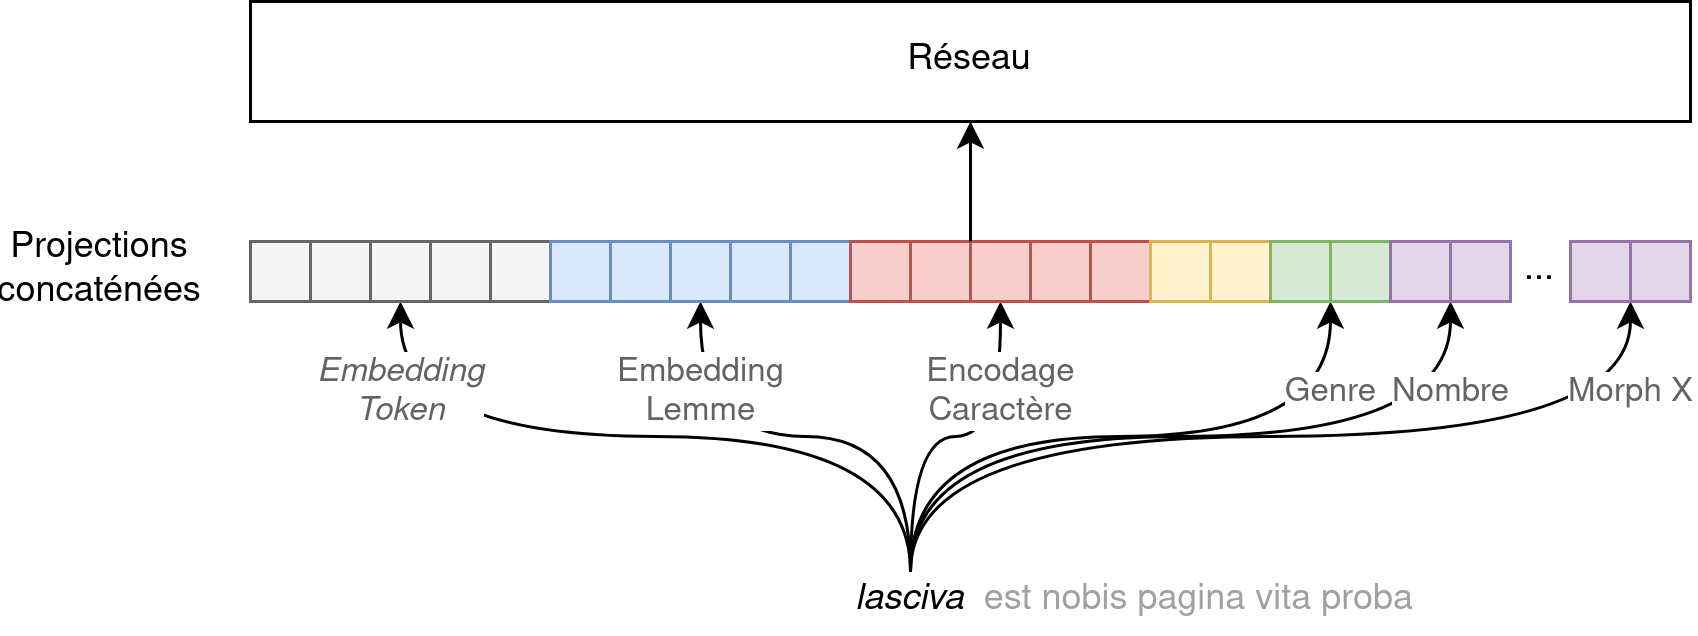
\includegraphics[width=\linewidth]{figures/chap4/Projection.drawio.png}
    \caption{Projection maximaliste réutilisant l'ensemble des informations à disposition du modèle (forme, lemme, caractère, traits morphologiques, POS): chaque information est toujours insérée dans le même ordre.}
    \label{fig:chap4:projection:morphosyntax}
\end{figure}
% ~  < 1 page ? (un gros paragraphe)

% POS et héritage des différentes problèmes cités plus hauts sur lemme / forme et perte d'information
% Problème des embeddings avec le mot

\subsubsection{Intégration des métadonnées}
\label{chap4:encodage:metadonnees}

\enquote{[Quand] la métaphore [est] \textit{in absentia}, elle instaure une connexion symbolique qui doit être identifiée par des conjectures concordantes sur le discours, le type de l'œuvre, le genre du texte, la hiérarchisation idiolectale des isotopies.\footcite[p. 98]{rastier_tropes_1994}}. Ces seuls mots de F.~Rastier indiquent combien la question du contexte est importante dans notre cas. Non content d'avoir dans nos textes de très nombreux passages du lexique de la sexualité, sur lesquels la machine ne devrait pas buter, la question de la métaphore et en général des tropes risque de se heurter à un mur: la machine ne connait pas ce que Martial est à la littérature latine, mais ne sait pas non plus, si on ne l'informe pas, que \enquote{\textit{Lasciva est nobis pagina}} est de Martial. La formalisation de ce contexte, de ces métadonnées, est alors répartie sur deux niveaux: un premier niveau qui concerne le document, l'œuvre (auteur, siècle, etc.) mais nous proposons de distinguer un second niveau, celui des \enquote{métadonnées de mots} (propriétés extra-linguistiques entre autres).

La problématique du contexte et de sa formalisation est encore assez récente dans les travaux de classification et de traitement séquentiel du langage en général. Parmi les rares publications existantes sur le sujet, on note celle de J. Kim et al.\footcite{kim_categorical_2019}. Les auteurs de cet article ajoutent l'information en parallèle au texte, en testant plusieurs moments d'insertion: les métadonnées sont d'abord projetées puis intégrées via des modifications de réseaux ou des concaténations. Le principe qui sous-tend cette insertion de la métadonnée par J. Kim est celui des goûts propres à un locuteur: cherchant à évaluer des critiques (culinaires en autres), les particularités de chaque locuteur peuvent s'exprimer à travers une relation lexique-évaluation notée. Ainsi, si une personne donne des critiques négatives en utilisant le terme \textit{épicé}, il est possible que ce terme ne relève pas des informations positives et aide à classer de futures des remarques. En ajoutant l'information liée à l'identité du locuteur, les auteurs montrent une augmentation du score atteignant jusqu'à +4.45 points de pourcent de la classification: la machine se met à prendre en compte l'idiolecte dans sa classification\footnote{L'exemple donné relève principalement de la partie lexicale d'un idiolecte, mais il est possible aussi que des faits de syntaxes puissent trahir les particularités propres de chaque critique.}.

% HERE 
Au-delà de l'intégration de l'idiolecte, la question du sociolecte peut-être tout aussi importante: \textit{virgo} n'a pas la même valeur pour un Romain chrétien et un romain païen, pour un romain du IVe siècle et du IIe d'avant notre ère. On retrouve d'ailleurs un usage des particularités d'un sociolecte dans l'une des études précédemment citées, celle de \textit{bot.zen}, où les chercheurs ont utilisé des plongements de mots dérivés de textes écrits par des apprenants de la langue anglaise\footcite{stemle_using_2018}. L'usage pour les plongements de mots d'une contextualisation temporelle\footcite{carlo_training_2019} ou géographique liées au contexte\footcite{gong_enriching_2020} n'est pas rare, contrairement à son utilisation dans des tâches de classification. Parmi les études sur l'usage de ces données, celle de Huang et Paul\footcite{huang_neural_2019} a la particularité de mettre au banc d'essais l'influence de l'injection de métadonnées temporelles dans les données pour des tâches de classification sur les sets habituels d'Amazon, Yelp, etc. Sur l'espace de trois à plus de dix ans, ils montrent et quantifient l'existence de changements de contexte et de déplacements sémantiques dans les datasets. L'usage d'informations temporelles montre une amélioration dans tous les cas, avec des augmentation de l'\textit{accuracy} allant d'un négligeable +0.4 à un impressionnant +3.8 points.

Enfin, il existe un dernier type d'information, en partie sociolectale, qui ne semble pas avoir intéressé outre mesure: celui de la prise en compte des \textit{sèmes} liés aux entités nommées, à savoir les lieux, les personnes, les divinités, les organisations, etc. Quand un romain parle d'Athènes, ou de Troie, un ensemble de sèmes peuvent apparaître: /Grèce/, /Épopée/, /Philosophie/, etc. Ces informations ne sont pas toujours déductibles des co-occurrences -- tous les locuteurs ne font pas comme les Américains en indiquant l'état dans lequel une ville se trouve (\enquote{Austin, Texas}), et encore, ce phénomène est réservé aux villes nord-américaines -- et peuvent relever d'une projection géographique, historique, littéraire -- les prostituées ont des noms grecs à Rome: qu'est-ce qu'un nom grec pour la machine ? Cette connaissance des propriétés des personnes (Martial et Sénèque viennent des régions espagnoles, Sénèque est un \enquote{conseiller politique} via sa position auprès de Néron), des lieux (localisation géopolitique) et des auteurs (Martial et Sénèque sont des auteurs dans des genres différents) ne peut transpirer entièrement et assez régulièrement pour que ces sèmes soient présents associé à leur nom. Les \textit{embeddings} étant une représentation de l'espace sémantique, des études pour fusionner des graphes de connaissances \enquote{encyclopédiques} avec ces derniers existent, qu'il s'agisse d'\textit{embeddings} classiques\footcite{wang_knowledge_2014} ou contextuels\footcite{zhang_ernie_2019}, mais leur application au latin semble encore assez lointaine. Dans \enquote{\textit{Semantic structure-based word embedding by incorporating concept convergence and word divergence}}\footcite{liu_semantic_2018}, Liu et ses collègues utilisent dans leur entraînement d'\textit{embeddings} un second objectif, celui de réduire la distance entre synonymes, hyponymes et hyperonymes issus d'un \textit{WordNet}: les gains en classification sur un corpus de presse dépassent leur meilleure \textit{baseline} de +0.4\% de score F1. Si un tel gain peut paraître minime, la limitation à un graphe sémantique tel que WordNet nous paraît dommage, surtout dans le cadre d'une classification d'articles de journaux, leur terrain d'expérimentation, où la relation entre entités nommées et leur classification ne peuvent être extraites du dictionnaire.


\subsection{Modèles et variations de modèles}

La construction du modèle pour cette recherche repose sur une architecture modulaire, permettant de tester de nombreuses hypothèses, tant du point de vue des modules d'encodage que des informations conservées. Du point de vue technique, l'ensemble de ces modèles sont construits sur la même architecture, avec des variations afin d'évaluer les apports des différentes informations et divers réseaux. Le plan du modèle est découpé en trois blocs principaux: 
\begin{itemize}
    \item un bloc de projection, qui vise à représenter chacune des unités d'information (mot, information morphologique, POS, métadonnée, etc.) dans l'espace;
    \item un bloc d'encodage, qui cherche à représenter le texte;
    \item une couche décisionnelle, qui produit la classification.
\end{itemize}
En fin de modèle, suivant qu'il s'agisse d'un entraînement ou d'un moment de prédiction, on trouvera une transformation de la décision en perte (\textit{loss}) ou en classification. Cette architecture est commune à l'ensemble des différents modèles étudiés jusqu'ici et nous permet d'y étudier des variations (\textit{cf.} Figure \ref{fig:chap4:Architecture}).

\begin{figure}
    \centering
    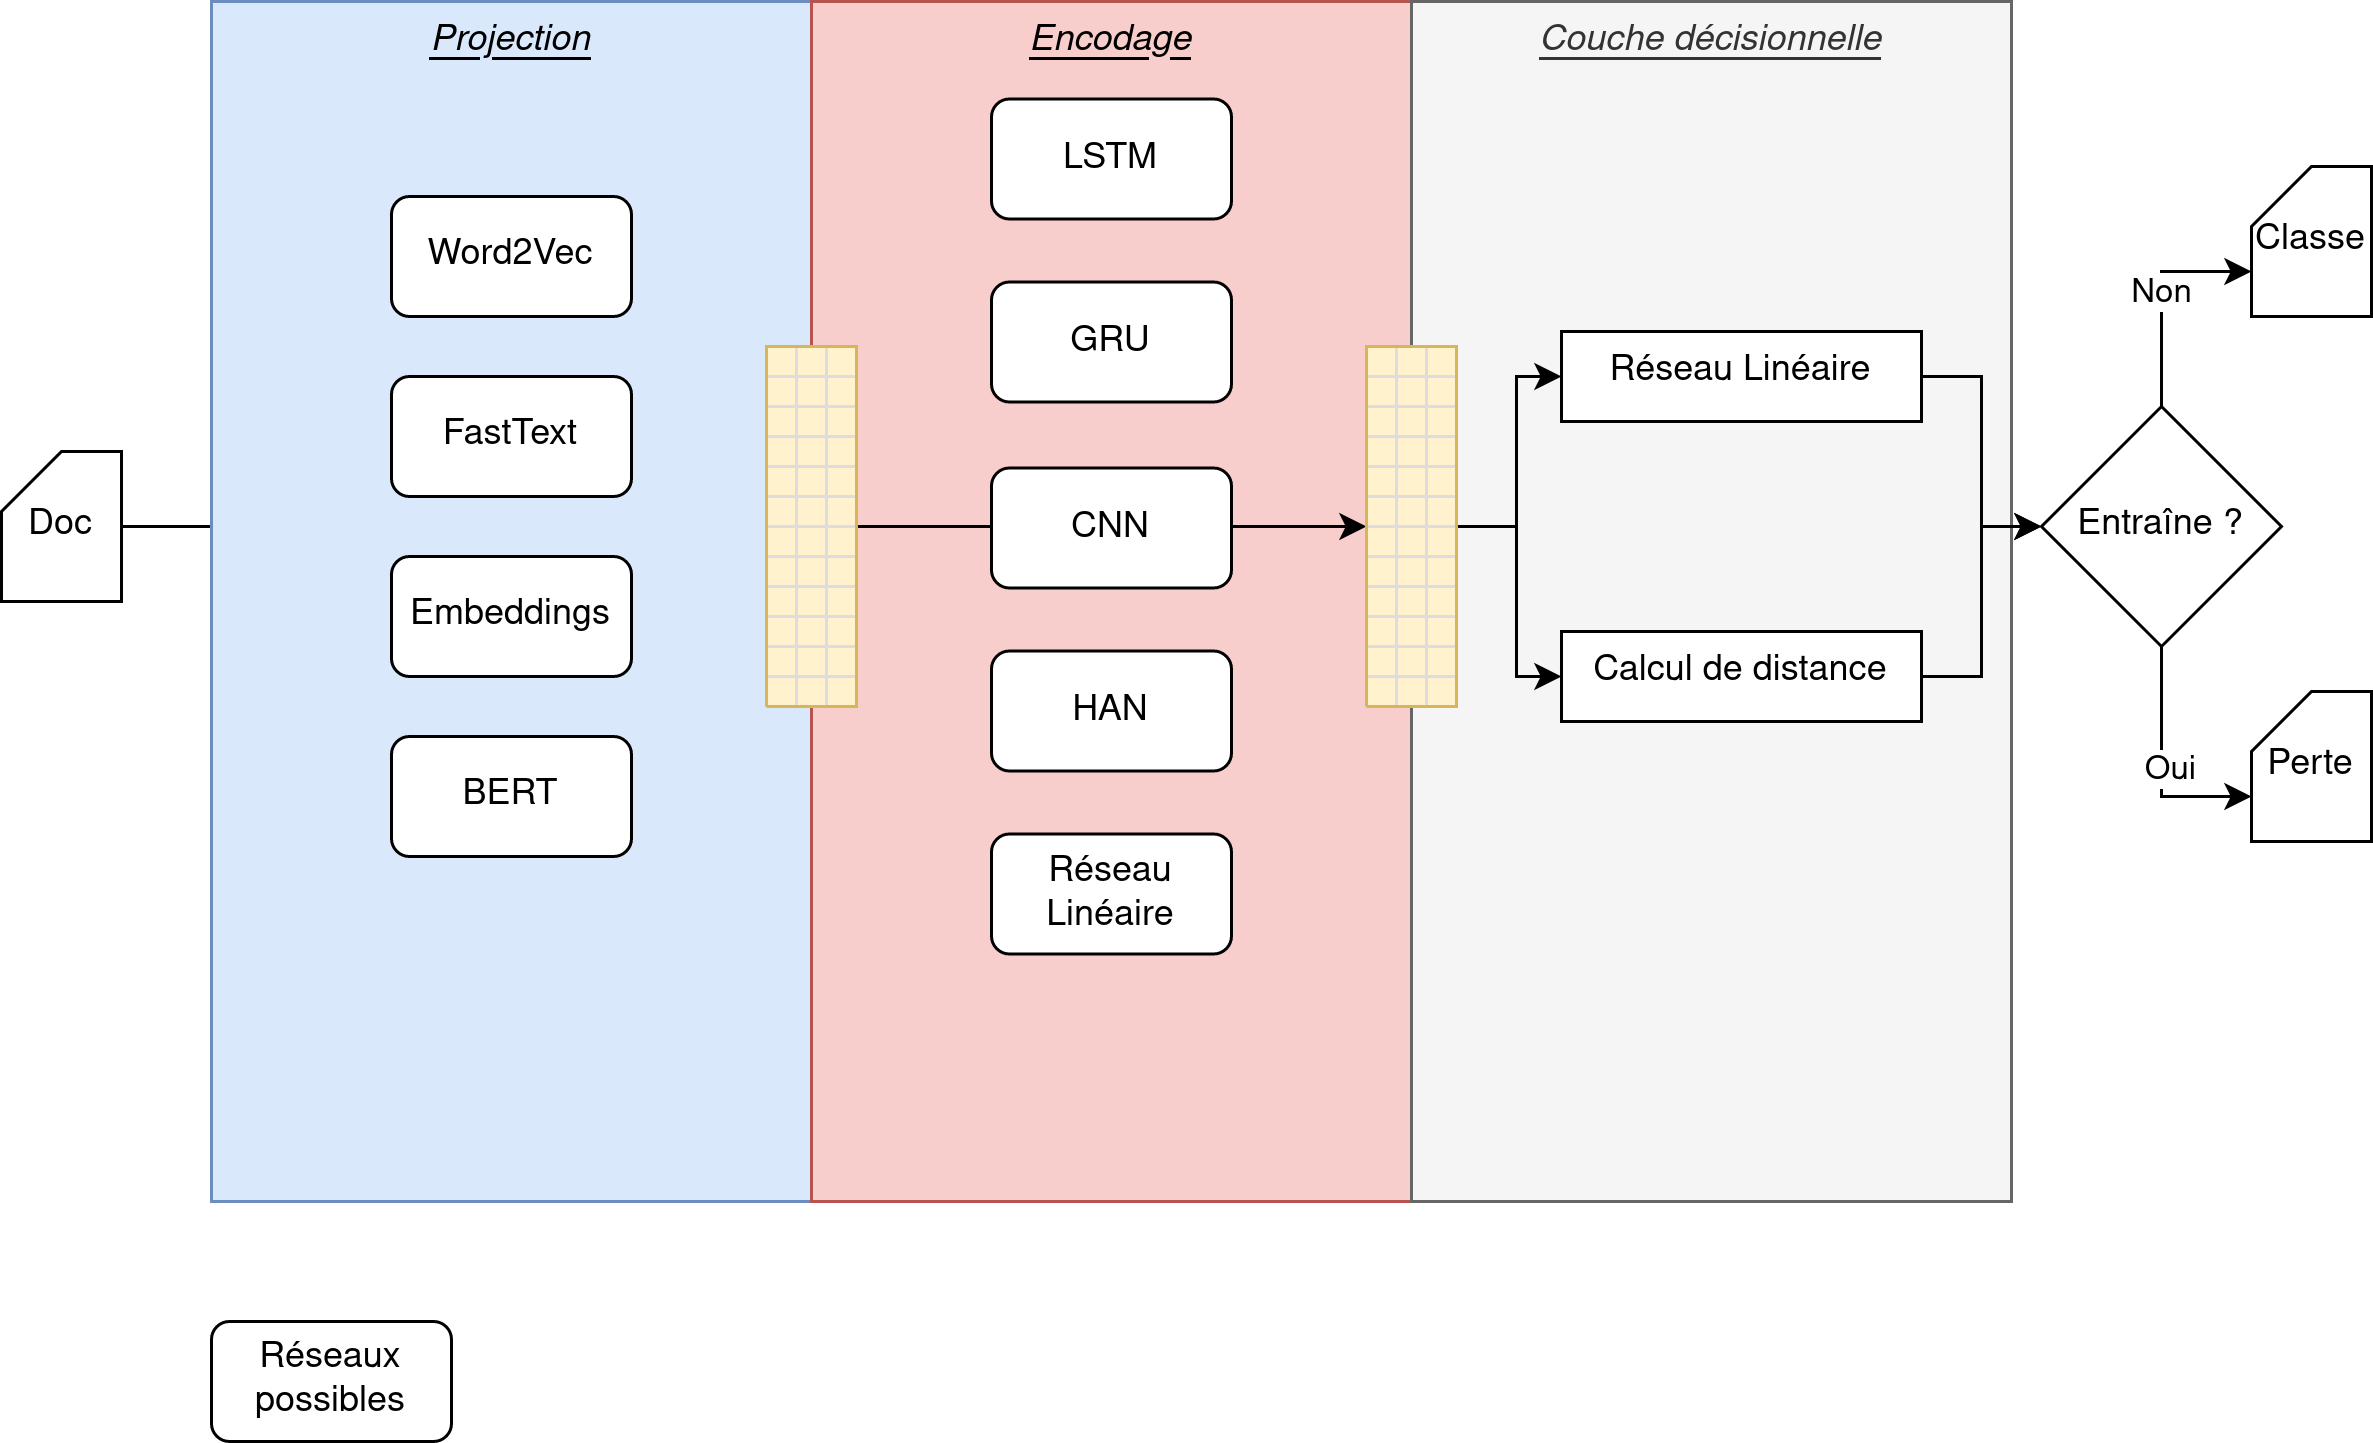
\includegraphics[width=\linewidth]{figures/chap4/architecture.png}
    \caption{Découpage de l'architecture générale. On distingue trois étapes: le passage des mots à des projections au niveau token, leur encodage au niveau phrase puis la partie de prise de décision. Selon que l'on entraîne ou que l'on utilise l'outil pour des prédictions, on obtient un score de perte ou de classification. Plusieurs modèles sont utilisables pour les deux premières couches de l'architecture.}
    \label{fig:chap4:Architecture}
\end{figure}

\subsubsection{Le bloc de projection}

La première forme de transformation s'effectue au niveau des tokens produits par \textit{Pie-Extended}: la séquence de tokens est fournie au modèle, qui utilise ou non l'ensemble des informations disponibles, à savoir les informations morphosyntaxiques, de formes ou de lemmes. Les formes et lemmes sont projetés par des embeddings pré-entraînés via Gensim\footcite{gensim} et non-entraînables basés sur \textit{FastText} ou \textit{Word2Vec} et de taille 200. Les catégories individuelles de morphosyntaxe (\texttt{Cas=X}, \texttt{Genre=X}, etc.) sont projetées sur une dimension assez faible de 3, tandis que la concaténation de ces tags (\texttt{Cas=X|Genre=Y}) est projetée sur une dimension de 20. En cas de projection au niveau caractère, disponible pour les lemmes et les formes, afin de prendre en compte la morphologie flexionnelle pour les caractères et les morphèmes non-flexionnels pour les deux, on utilise un encodage au niveau caractère utilisant un réseau LSTM avec une \textit{hidden size} de 150, deux couches et un \textit{dropout} de 30\%. L'ensemble des projections est concaténée en un seul vecteur pour chaque token (\textit{cf.} figure \ref{fig:chap4:projection:morphosyntax}).

On peut ajouter à cette transformation des formes, lemmes et informations morphosyntaxique un encodage via le module BERT latin, développé par D. Bamman et P. J. Burns. Deux problèmes se sont posés avec cette utilisation, dont un n'a pu être résolu. D'une part, le module pose un problème d'ingénierie: l'outillage entourant le modèle BERT est peu documenté, lent et repose sur des versions plutôt anciennes de certains outils qui ont parfois été un véritable puzzle de dépendances\footnote{CLTK posant notamment de gros problèmes sur ce point.}. Ensuite, il y a un véritable problème dans le pré-traitement de l'information: les deux auteurs du projet ont utilisé la tokenisation de CLTK en pré-traitement, que nous avons voulu à tout prix éviter, car, basée sur des règles, elle a une forte propension à interpréter chaque morphème final \textit{-ne} comme un clitique, de même que les \textit{-ve} ou les \textit{-que} (par exemple, \textit{observatio-ne} et \textit{observatio-ve} sont systèmatiquement tokenizés en deux morceaux, bien que le premier est souvent un simple ablatif). L'usage de ce \textit{pre-tokenizer} est par ailleurs une bizarrerie algorithmique du point de vue de BERT: l'objectif même de ce dernier, avec ses systèmes de tokenization reposant sur des \textit{sous-tokens}, est de pouvoir gérer ce type de phénomènes. Par exemple, dans le cadre du modèle BERT allemand de Chan et al.\footcite{chan_german_2019}, on retrouve ainsi logiquement traités par le \textit{tokenizer} les sous-tokens grammaticaux \texttt{\#\#ge}, les préfixes \texttt{\#\#be} et \texttt{\#\#ver}, sans pré-traitement manuel par les chercheurs: \textit{vergenommen} est ainsi transcrit en \texttt{\#\#ver + \#\#genommen}\footnote{\textit{nehmen} ayant de nombreux dérivés et étant relativement fréquent dans la langue allemande, il n'est pas étonnant que le composant \texttt{\#\#genommen} existe permettant ainsi une construction économique en bi-gram pour \textit{abnehmen, vernehmen, etc.}}. Nous nous sommes ainsi refusé à utiliser la prétokenization faussée de CLTK, espérant que le composant de tokenization de BERT soit suffisant pour pallier à cette situation\footnote{Mais la différence de tokenization pousse tout de même au final à l'incapacité d'aligner -- simplement -- les tokens.}. Enfin, en cas d'usage de projections via BERT et de projection classiques par \textit{embeddings} non contextuels, on utilise soit une concaténation des vecteurs BERT avec les vecteurs issus des plongements non contextuels, soit une réduction via une réduction en réseau linéaire.

\subsubsection{Le bloc d'encodage}
\label{part:chap4:architectures:variations-architectures:encodage}

Le bloc d'encodage est probablement le plus simple des trois blocs. Il prend comme entrée les projections unitaires précédentes -- au niveau token -- pour produire une projection séquentielle -- au niveau texte. On utilise majoritairement dans ce contexte des réseaux récurrents, LSTM et GRU, en mode bi-directionnel, avec un \textit{dropout} de 30\% et et une taille de 50 par direction. Alternativement aux réseaux récurrents, on retrouve aussi une option pour un réseau convolutionnel, avec des tailles de filtres de 2 à 5 (n-grams) et 5 filtres, un filtrage par MaxPool et une activation par ReLU.

Si ces réseaux sont communs, la recherche en classification a fait émerger d'autres moyens d'obtenir une représentation en augmentant ces modules. Le plus important de ceux-ci est sans aucun doute celui décrit dans \textit{Hierarchical Attention Networks for Document Classification}(\textit{HAN})\footcite{yang_hierarchical_2016}, présenté en 2016, basé sur des réseaux récurrents et qui sera décliné avec un modèle convolutionnel (CHAN) en 2019\footcite{gao_hierarchical_2018}. Ce modèle est fondé autour d'un réseau d'encodage récurrent et d'un systême de pondération appelé \enquote{attention}. Cette \textit{attention} est une partie du modèle entraînée en même temps que l'encodeur dont l'objectif est de disperser sur l'ensemble de la phrase une mesure d'importance. Une phrase possédant 100\% de poids, ses mots les moins importants pour la classification seront dotés d'une \textit{attention} très réduite, proche de 0, tandis que ceux qui permettent d'aider au plus le modèle seront accrédité d'une très grosse partie du poids. Par exemple, dans \enquote{\textit{Lasciva est nobis pagina, vita proba}} (\enquote{Nos pages sont lascives, notre vie probe}), dans le cadre de notre corpus, les mots présentant l'isotopie de la sexualité pourraient être en premier lieu \textit{lasciva} puis, peut-être, \textit{proba}, dans son jeu d'opposition /lascif/ contre Non(/lascif/). Les termes \textit{vita} et \textit{pagina} n'ont pas ou peu d'importance directe pour notre sujet, tandis que \textit{est}, \textit{nobis} et les signes de ponctuation n'en ont absolument aucune à priori. Cette importance des termes se traduit par une attention forte, tandis que le caractère négligeable des autres unités se traduit par une attention quasi-nulle.

Ce complément pour l'encodage séquentiel a aussi l'avantage de fournir au lecteur un outil d'analyse de ce qu'apprend le modèle. En ajoutant aux informations classiquement produites par le modèle, telles la classification les pondérations de l'attention, il met en exergue les traits saillants détectés. Cet outil a deux intérêts majeurs. D'une part, à travers les jeux de répétition qui auraient échappé à l'œil humain, il peut permettre de questionner une analyse plus manuelle des sèmes actualisés par une isotopie: les mots portants ces sèmes sont identifiés par le phénomène d'attention et amènent à interroger leur rôle. D'autre part, il peut permettre de détecter des phénomènes que nous qualifierions de \enquote{triche} mais qui relève bien du sur-apprentissage: dans notre cas, il nous est arrivé de trouver que pour les textes d'une édition en particulier, l'obèle de l'édition était un token spécifique au corpus positif, que le modèle a ainsi interprété comme trait saillant. Ce phénomène peut se retrouver avec d'autres mots, dont les actualisations /sexuel/ ne sont pas les plus courantes: c'est à cet endroit que l'équilibrage du corpus est important.

Dans le cadre de notre usage de BERT, il existe deux situations: une première où BERT est la seule projection utilisée, une second où BERT est employé avec d'autres projections.

Pour la première des deux, il existe plusieurs stratégies, dont la plus commune consiste à exploiter les tokens de délimitation des phrases \texttt{[CLS]} et \texttt{[SEP]} qui représentent respectivement le début de la séquence et la fin de la séquence. BERT proposant des plongements de token contextualisés, ces deux éléments ont la particularité de contenir une information contextualisée sur la phrase sans porter eux-mêmes de signification propre. Parmi les autres stratégies, on distingue les fonctions de réduction par moyenne (\textit{Reduce Mean}) et par valeur maximum (\textit{Reduce Max}), ainsi qu'une combinaison des deux via concaténation. Ces méthodes sont appelées méthodes de \textit{pooling}. BERT étant son propre réseau neuronal avec plusieurs couches, certains chercheurs et services recommandent d'éviter d'utiliser la dernière couche si il n'y a pas de ré-entraînement\footnote{\textit{Cf.} \url{https://github.com/hanxiao/bert-as-service/blob/master/docs/section/faq.rst\#bert-has-12-24-layers-so-which-layer-are-you-talking-about}}: elle serait ainsi trop liée à l'objectif initial de BERT (prédiction de mot ou de phrase suivante) et servirait donc de mauvaise ressource pour des tâches différentes. Afin d'ajouter une couche d'entraînement supplémentaire, on peut passer cette représentation via BERT dans un réseau ayant pour objectif de réduire l'information (couche linéaire): ainsi, d'un vecteur de 768 ou 1536 (\textit{MeanMax}) on passe alors à 256 avant d'entrer dans le bloc décisionnel. Il est aussi possible d'utiliser la projection contextualisée dans des réseaux plus traditionnels, tels que GRU, HAN ou LSTM.

\begin{figure}[ht]
    \centering
    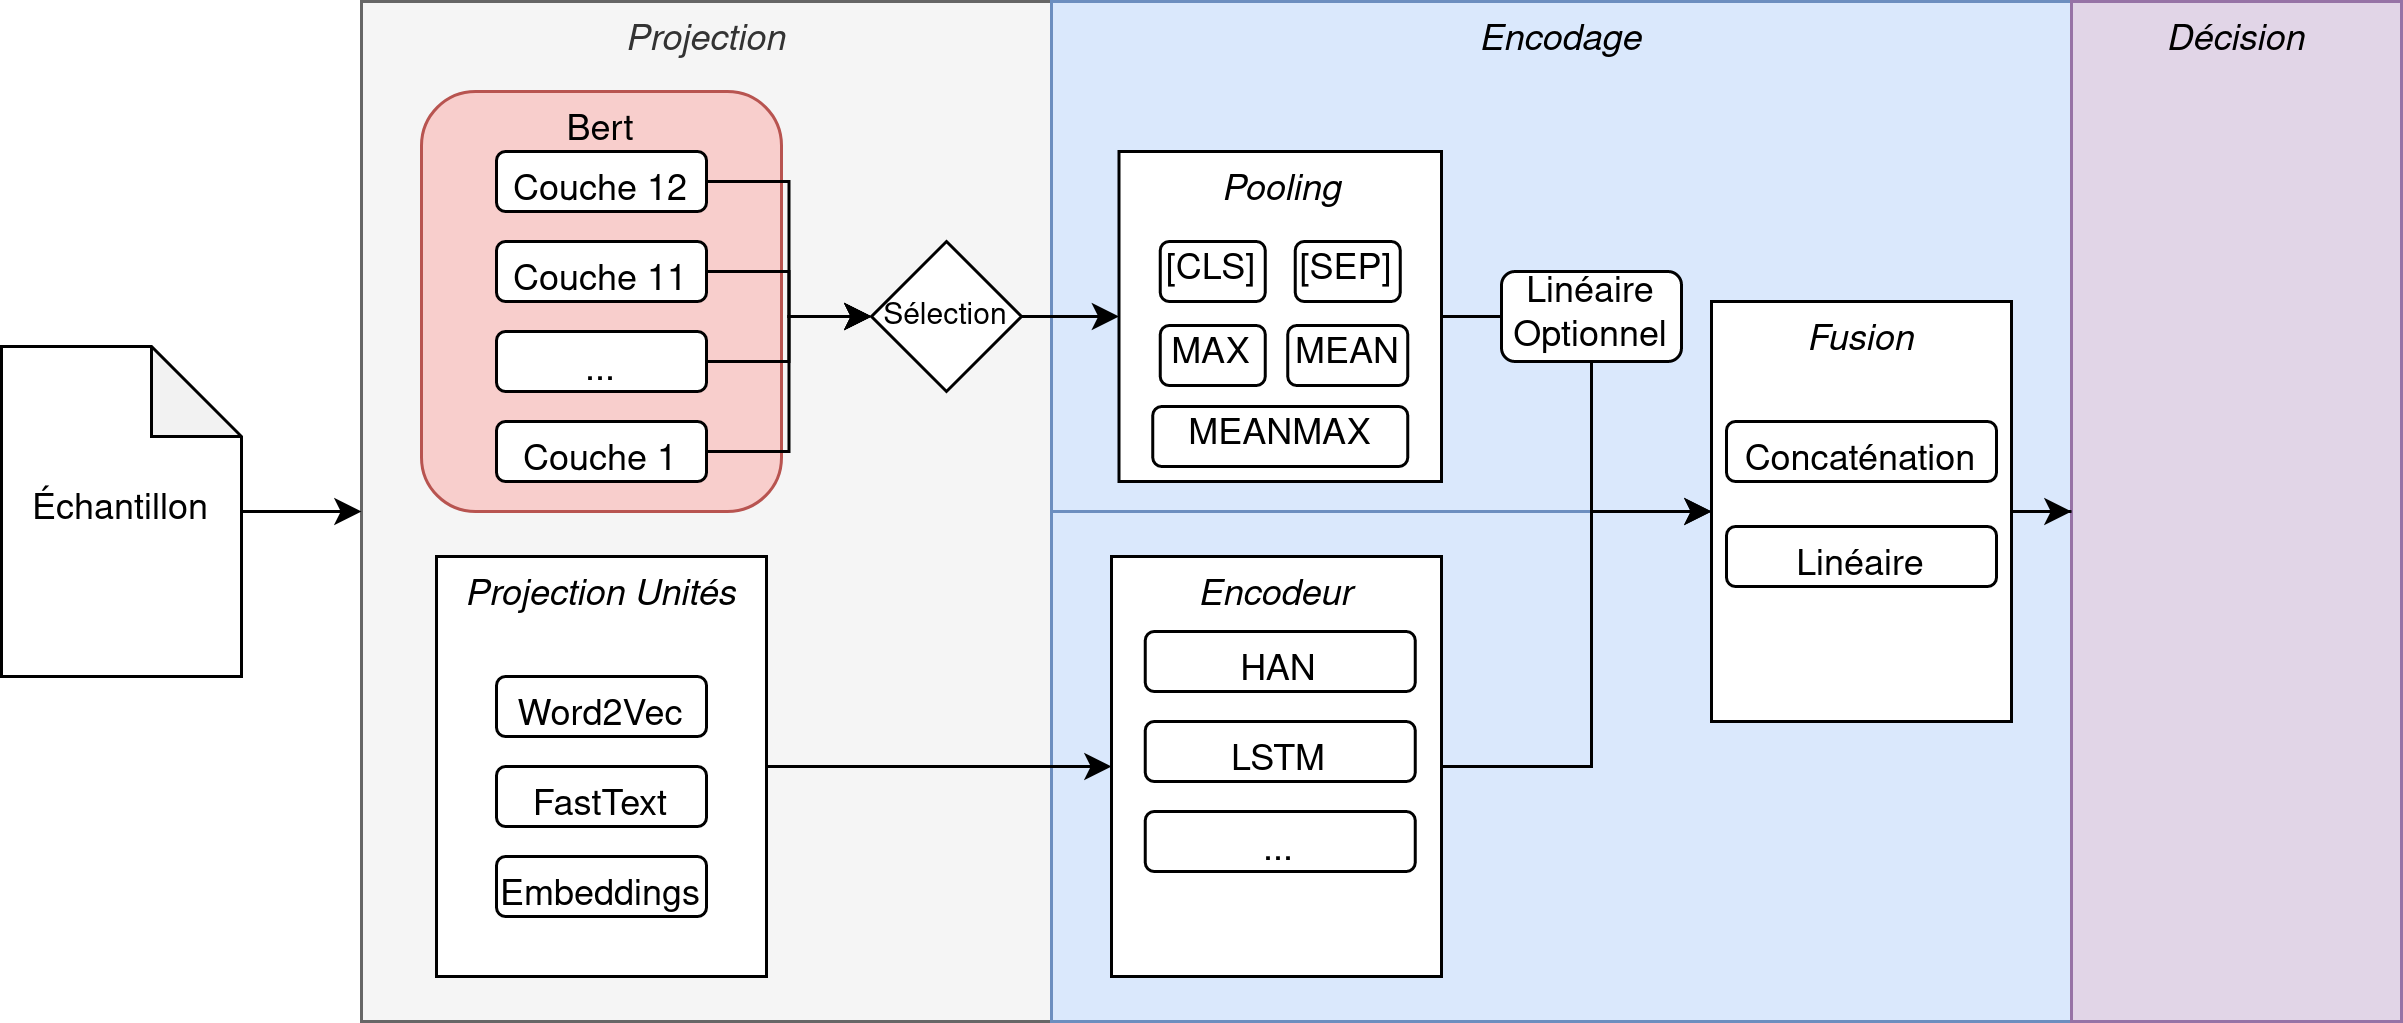
\includegraphics[width=\linewidth]{figures/chap4/BertZoom.png}
    \caption{Zoom sur les possibilités et relations entre projection et encodage.}
    \label{fig:chap4:zoom-projection}
\end{figure}

Pour le second cas, où projections par BERT et projections par embeddings non-contextualisés se complètent, on procède ainsi: la projection de BERT est effectuée comme dans le cas précédent via une méthode de \textit{pooling} et une optionnelle réduction linéaire, tandis que la projection traditionnelle est encodée via l'un des réseaux décrits plus hauts, récurrent ou convolutionnel. Les deux entrées sont ensuite ou concaténées, ou réduite via une couche linéaire, afin de fournir les deux informations (\textit{cf.} figure \ref{fig:chap4:zoom-projection}).

\subsubsection{Classification, similarité: la couche décisionnelle et les méthodes d'entraînement}

Après avoir projeté les unités et encodé la séquence, le modèle passe à la dernière phase de la classification, celle de la couche décisionnelle. Cette couche décisionnelle se décline en deux architectures principales: l'une, classique, orientée classification via une projection linéaire; l'autre, plus particulière, orientée comparaison.

La première architecture est assez simple: elle prend en entrée l'information encodée par le bloc précédent et, via une couche linéaire, réduit celle-ci en un vecteur de taille 2, où chacune des cordonnées du vecteur représente une classe, ici \texttt{isotopie sexuelle} ou \texttt{absence de cette isotopie}. Pour produire la classification, on applique au vecteur une fonction \textit{softmax}, qui a la particularité d'équilibrer les valeurs telles que la somme des valeurs du vecteur soit égale à 1 en conservant la hiérarchisation des valeurs (le score le plus haut reste le plus haut). Pour la perte, on applique une traditionnelle \textit{Cross Entropy Loss}.

La seconde architecture est plus complexe, car elle recoupe plusieurs variations. Son principe fondamental est de comparer la sortie du bloc d'encodage -- donc l'échantillon encodé -- avec un ou plusieurs échantillons encodés dont la classe est connue. Cette méthode, dite de réseau siamois, consiste donc à faire passer dans le même réseau les données et d'inférer une classe en fonction de la proximité d'un texte avec un ou plusieurs autres textes. 


\begin{figure}[ht]
    \centering
    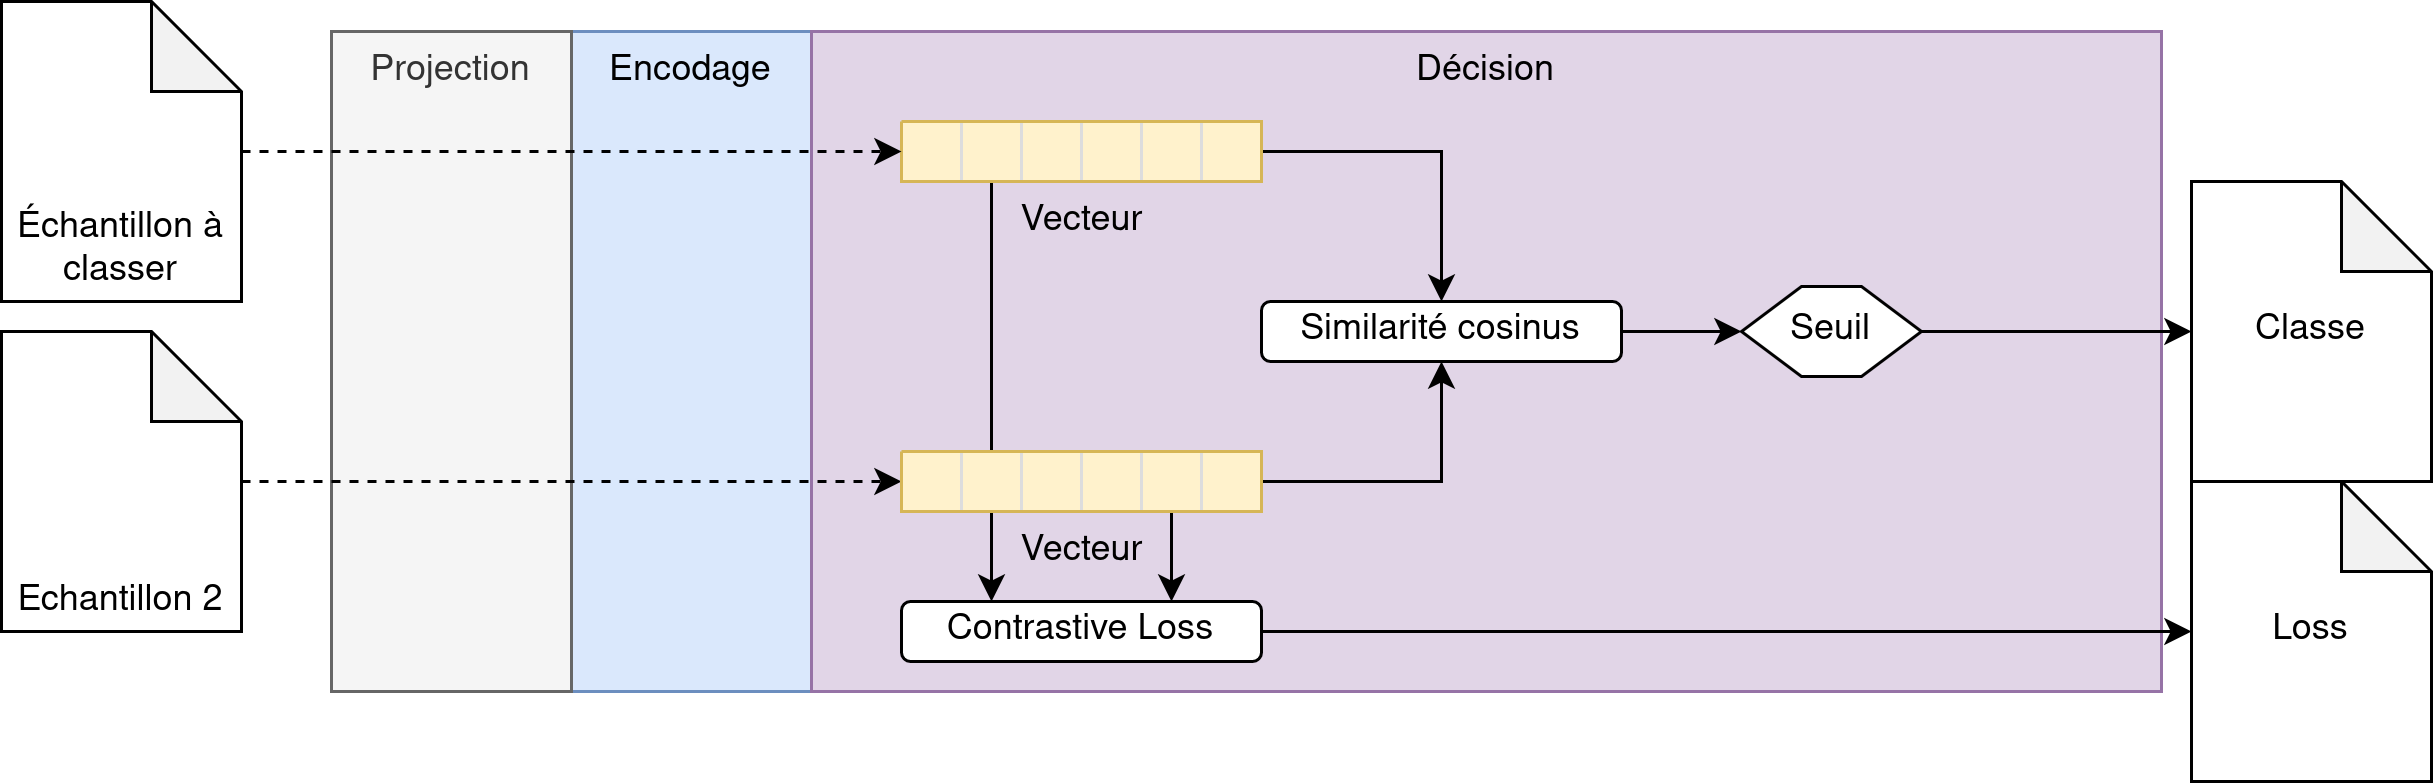
\includegraphics[width=\linewidth]{figures/chap4/contrastive.png}
    \caption{Schéma de fonctionnement d'un réseau siamois à double échantillons.}
    \label{fig:chap4:reseau:ContrastiveLoss}
\end{figure}

La première variation des réseaux siamois utilise deux échantillons, un que l'on souhaite classer, et un dont on connait la classe, ci-après le comparant. Une fois encodés, on les compare à l'aide d'une fonction de similarité cosinus: si la similarité entre les deux dépasse un seuil, fixé arbitrairement pour nous à 0.6, l'échantillon est considéré comme appartenant à la classe du comparant. Au contraire, si le seuil n'est pas atteint, cette appartenance est rejetée. Pour la perte (\textit{loss}), qui permet de diriger l'entraînement, on utilise une \textit{contrastive loss}\footcite[Entre autres, ]{khosla_supervised_2021} qui prend directement comme paramètres les encodages d'échantillons pour calculer un écart entre les deux (\textit{cf.} image \ref{fig:chap4:reseau:ContrastiveLoss}). La seconde variation des réseaus siamois utilise trois échantillons, dont deux comparants. Ces deux échantillons de comparaison ne doivent pas représenter la même classe, et l'un d'eux doit, au possible, avoir la même classe que celui avec lequel on entraîne le modèle. On calcule la distance entre les comparants encodés et l'échantillon via une distance euclidienne, et l'on attribue la classe du comparant le plus proche à l'échantillon évalué. Pour la perte, on utilise une perte appelée \textit{Triplet Margin Loss}\footcite{hermans_defense_2017} qui est alors calculée directement à partir des données issus de la phase d'encodage.

\begin{figure}[ht]
    \centering
    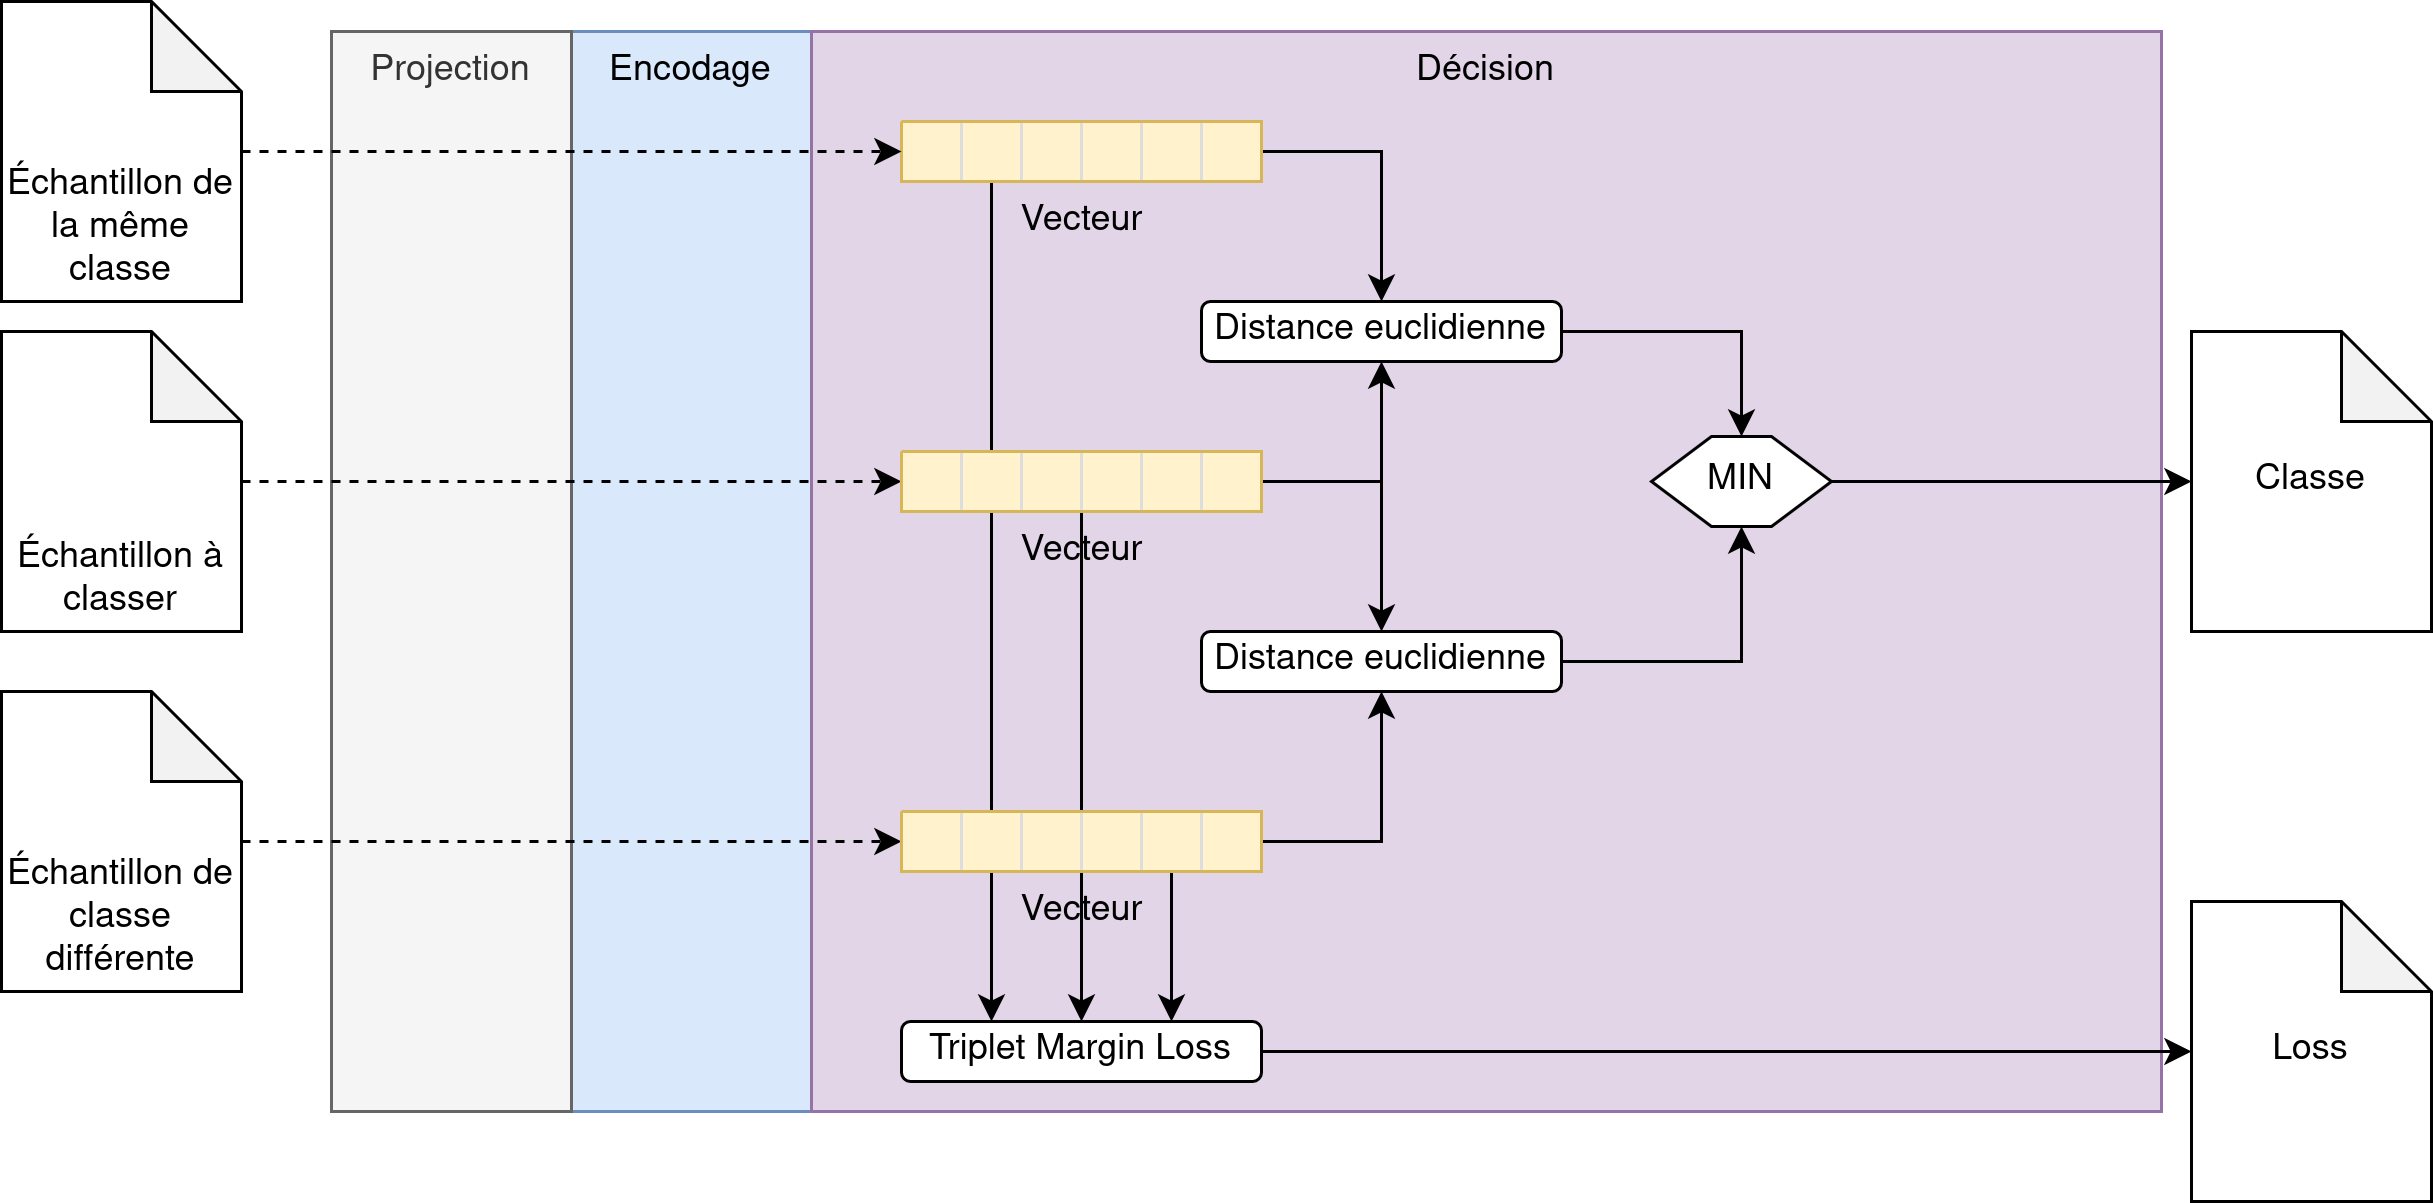
\includegraphics[width=\linewidth]{figures/chap4/triplet.png}
    \caption{Schéma de fonctionnement d'un réseau siamois à triple échantillons.}
    \label{fig:chap4:reseau:Triplet}
\end{figure}

Pour ces deux variations, les stratégies d'entraînement ou de prédiction peuvent varier. La méthode la plus simple, à la fois algorithmiquement et méthodologiquement, est la sélection manuelle d'un ou plusieurs représentant(s) par classes: à chaque fois que le modèle entraîne un échantillon, il tire au hasard un représentant positif ou négatif avec lequel les distances seront calculées. Ces représentants sont ensuite sauvegardés avec le modèle afin de pouvoir continuer à effectuer des prédictions. Une autre méthode d'échantillonnage consiste à prendre tous les binômes ou triplets possibles d'un même ensemble d'échantillons et de les utiliser comme données à évaluer. Il existe cependant des méthodes d'échantillonages qui cherchent à mathématiquement maximiser les erreurs afin de rendre l'apprentissage le plus difficile possible, nous en testons deux: le \textit{BatchEasyHard} de Xuan et al.\footcite{xuan_improved_2020}, qui cherche à trouver des triplets dont le comparant positif est simple mais le comparant négatif est complexe, et le \textit{BatchHard} de Hermans et al.\footcite{hermans_defense_2017} qui cherche par défaut les triplets les plus complexes à classer pour chaque échantillon\footnote{Nous utilisons les implémentations de ces échantillonneurs issu es de la librairie \texttt{pytorch-metric-learning}, \textcite{musgrave2020pytorch}}. 

\subsubsection{Le cas particulier de l'inclusion des métadonnées}
\label{chap4:part2:metadata}

Nous parlions en \ref{chap4:encodage:metadonnees} de la possibilité et de la potentielle importance d'incorporer les métadonnées en tant qu'elles apportent des identificateurs extra-linguistiques pour les idiolectes et sociolectes. Nous approchons le problème de deux manières différentes: d'une part, à travers l'intégration de tokens de métadonnées dans la séquence, d'autre part via l'utilisation de modules modifiés en suivant les travaux de \footcite{kim_categorical_2019}. Quatre domaines de métadonnées peuvent être injectés, à savoir: la période d'écriture (le siècle), l'auteur, la structure logique de citation (par exemple: chapitre,section) et la forme d'écriture (prose ou vers).

Dans le cas de token de métadonnées, les vecteurs de mots sont nécessairement entraînables et non figés par le pré-entraînement, et on ajoute au vocabulaire des ces différents modèles de de nouveaux éléments suivants une syntaxe spécifique, telle \texttt{$[$Date:1$]$}. Ces tokens sont traités sans POS et sans morphologie, leur lemme étant identique à leur forme. Ils sont ensuite traités comme le reste des tokens par les réseaux d'encodage.

Dans le second cas, les métadonnées sont projetées dans des espaces propres de taille 64 comme des embeddings. Ces données sont ensuite injectées dans des modules modifiés: nous proposons ainsi, grâce aux travail de Kim et al. des modifications des réseaux LSTM, HAN basé sur LSTM et de la couche linéaire pour la partie décisionnelle. De même que dans l'article original, cette information ne peut être injectée qu'une seule fois dans le réseau par échantillon.

\section{Classement des architectures et de leurs modèles}
\label{chap4:part3}

L'entraînement de modèles et la construction d'architectures sont un processus itératif et exploratoire: il s'agit de tester des hypothèses de modèles, des hypothèses de paramétrages de modèles, puis d'aller dans l'une ou l'autre direction qui semble apporter les meilleures réponses. Rendre compte de ce processus, et de ses résultats, n'est pas une mince affaire: la chronologie a un rôle dominant dans la sélection de modèles qui survivront aux différents tests.

\subsection{Méthodes d'entraînement et résultats principaux}

\subsubsection{Méthode de sélection globale}

Pour définir les meilleurs modèles, nous avons procédé par test d'architecture: les réflexions qui suivront, leurs analyses, ont enrichi cette méthode continuellement pendant nos expériences. Le résultat produit une grande variété d'architectures: vingt-huit sont composées de couches linéaires et vingt-huit autres configurées en réseau siamois, que l'on multiplie par deux -- en faisant varier la taille de la couche d'encodage entre 128 et 256 -- pour atteindre les cent~douze configurations testées au total. À partir de ce premier set d'entraînement, nous récupérons les cinq meilleures configurations toutes couches décisionnelles confondues. Cette sélection d'architecture fait l'objet d'une seconde salve d'entraînements où chacune d'entre elles fait l'objet de dix entraînements: cette multiplication des entraînements permet prendre en compte les possibles variations de ces derniers (\textit{cf.} figure~\ref{fig:chap4:50configurations}). Chaque architecture est testée avec les mêmes hyperparamètres pour l'entraînement: un \textit{learning rate} de $1e^{-5}$, une taille de \textit{batch} de 4 et 20 \textit{epochs} au maximum. 

\begin{figure}[ht]
    \centering
    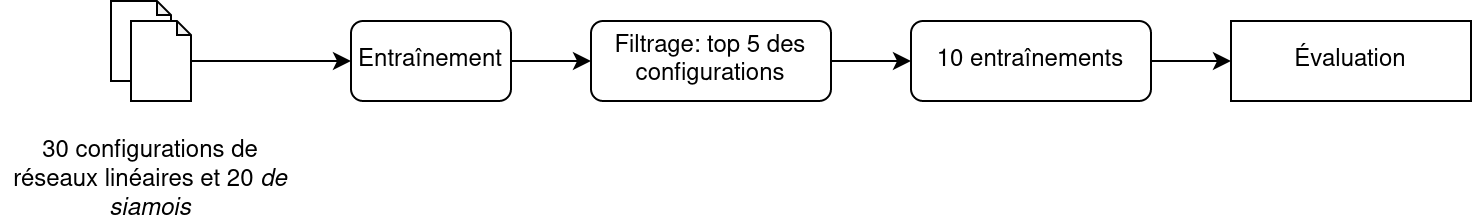
\includegraphics[width=\linewidth]{figures/chap4/50config.png}
    \caption{Résumé de la méthode de sélection des configurations}
    \label{fig:chap4:50configurations}
\end{figure}

% En cas de résultats plus bas que ce que promet la littérature scientifique, d'autres tests d'architectures ou d'outillages peuvent s'ajouter à ces méthodes. Si de nouvelles configurations ont dû être comparées, elles sont entraînées elles aussi dix fois.
% Commencer par les métadonnées en fait
% Ensuite, séparer BERT et Non Bert

% Expliquer itération: un run par archi. d'abord, pour évacuer les mauvaises archis.

\subsubsection{Modèles enrichis par métadonnées}

Comme nous l'avions vu en \ref{chap4:encodage:metadonnees}, la publication de J. Kim et al.\footcite{kim_categorical_2019} propose une méthode simple d'intégration de métadonnées dans l'entraînement de modèles de classification de texte permettant de prendre en compte les identités des locuteurs. Cette méthode, reposant donc sur une identification même partielle de traits idiolectaux ou sociolectaux, a été testée sur notre corpus avec quatre métadonnées: l'identité de l'auteur, le siècle de vie de l'auteur, la structure logique de citation de l'oeuvre et la forme de cette dernière\footnote{\textit{Cf.} section \ref{chap4:part2:metadata}}. 

\begin{table}[ht]
\centering
\resizebox{\linewidth}{!}{%
\begin{tabular}{@{}lllllllll@{}}
\toprule
Rang & Score F1 (Positif) & Rappel (Positif) & Précision (Positif) & Couche enrichie & Réseau d’encodage & Métadonnées utilisées              \\ \midrule
1    & 86.05\%            & 87.25\%          & 84.88\%             & Linéaire        & HAN               & Toutes                             \\
2    & 84.45\%            & 80.08\%          & 89.33\%             & Linéaire        & HAN               & Toutes                             \\
3    & 84.15\%            & 88.84\%          & 79.93\%             & Linéaire        & HAN               & Toutes                             \\
4    & 84.12\%            & 81.27\%          & 87.18\%             & Linéaire        & HAN               & Forme,Siècle,Structure de Citation \\
5    & 83.79\%            & 79.28\%          & 88.84\%             & Linéaire        & HAN               & Forme,Siècle,Structure de Citation \\
6    & 83.30\%            & 78.49\%          & 88.74\%             & LSTM            & LSTM              & Toutes                             \\
7    & 83.17\%            & 83.67\%          & 82.68\%             & Linéaire        & HAN               & Forme,Siècle,Structure de Citation \\
8    & 82.08\%            & 78.49\%          & 86.03\%             & Linéaire        & HAN               & Forme,Siècle,Structure de Citation \\
9    & 81.82\%            & 78.88\%          & 84.98\%             & Linéaire        & HAN               & Toutes                             \\
10   & 81.65\%            & 78.88\%          & 84.62\%             & LSTM            & LSTM              & Forme,Siècle,Structure de Citation \\
11   & 81.24\%            & 78.49\%          & 84.19\%             & LSTM            & LSTM              & Forme,Siècle,Structure de Citation \\
12   & 81.08\%            & 77.69\%          & 84.78\%             & LSTM            & LSTM              & Forme,Siècle                       \\
     & …                  &                  &                     &                 &                   &                                    \\
23   & 78.54\%            & 72.91\%          & 85.12\%             & Aucune          &                   & Aucune                             \\ \bottomrule
\end{tabular}%
}
\caption{Résultats ordonnés par le score F1 de la catégorie positive des meilleurs modèles sur la recherche de meilleure architecture. Les onze premiers modèles utilisent toutes les métadonnées, ou toutes sauf la métadonnée auteur. Les auteurs paramètres n'ont pas d'effet aussi marquant sur le classement.}
\label{tab:chap4:resultats-metadata}
\end{table}

\begin{table}[ht]
\centering
\begin{tabular}{l|r|r}
                                   & \multicolumn{2}{r}{Entraînements} \\ \hline
                                   & Tous & Top 25 (Score F1 Positive) \\ \hline
Toutes                             & 32   & 9                          \\
Forme,Siècle,Structure de Citation & 16   & 8                          \\
Forme,Siècle                       & 20   & 7                          \\
Token de Métadonnées               & 4    & 0                          \\
Aucune                             & 40   & 2                          \\ \hline
\end{tabular}
\caption{Répartitions des configurations par usage des métadonnées. $p=3,54^{-14}$, on peut rejeter l'hypothèse nulle: la variation de distribution est significative, l'usage des toutes les métadonnées ou de trois d'entre elles ont un impact sur les résultats finaux.}
\label{tab:chap4:metadata-p-value}
\end{table}

\begin{figure}[ht]
    \centering
    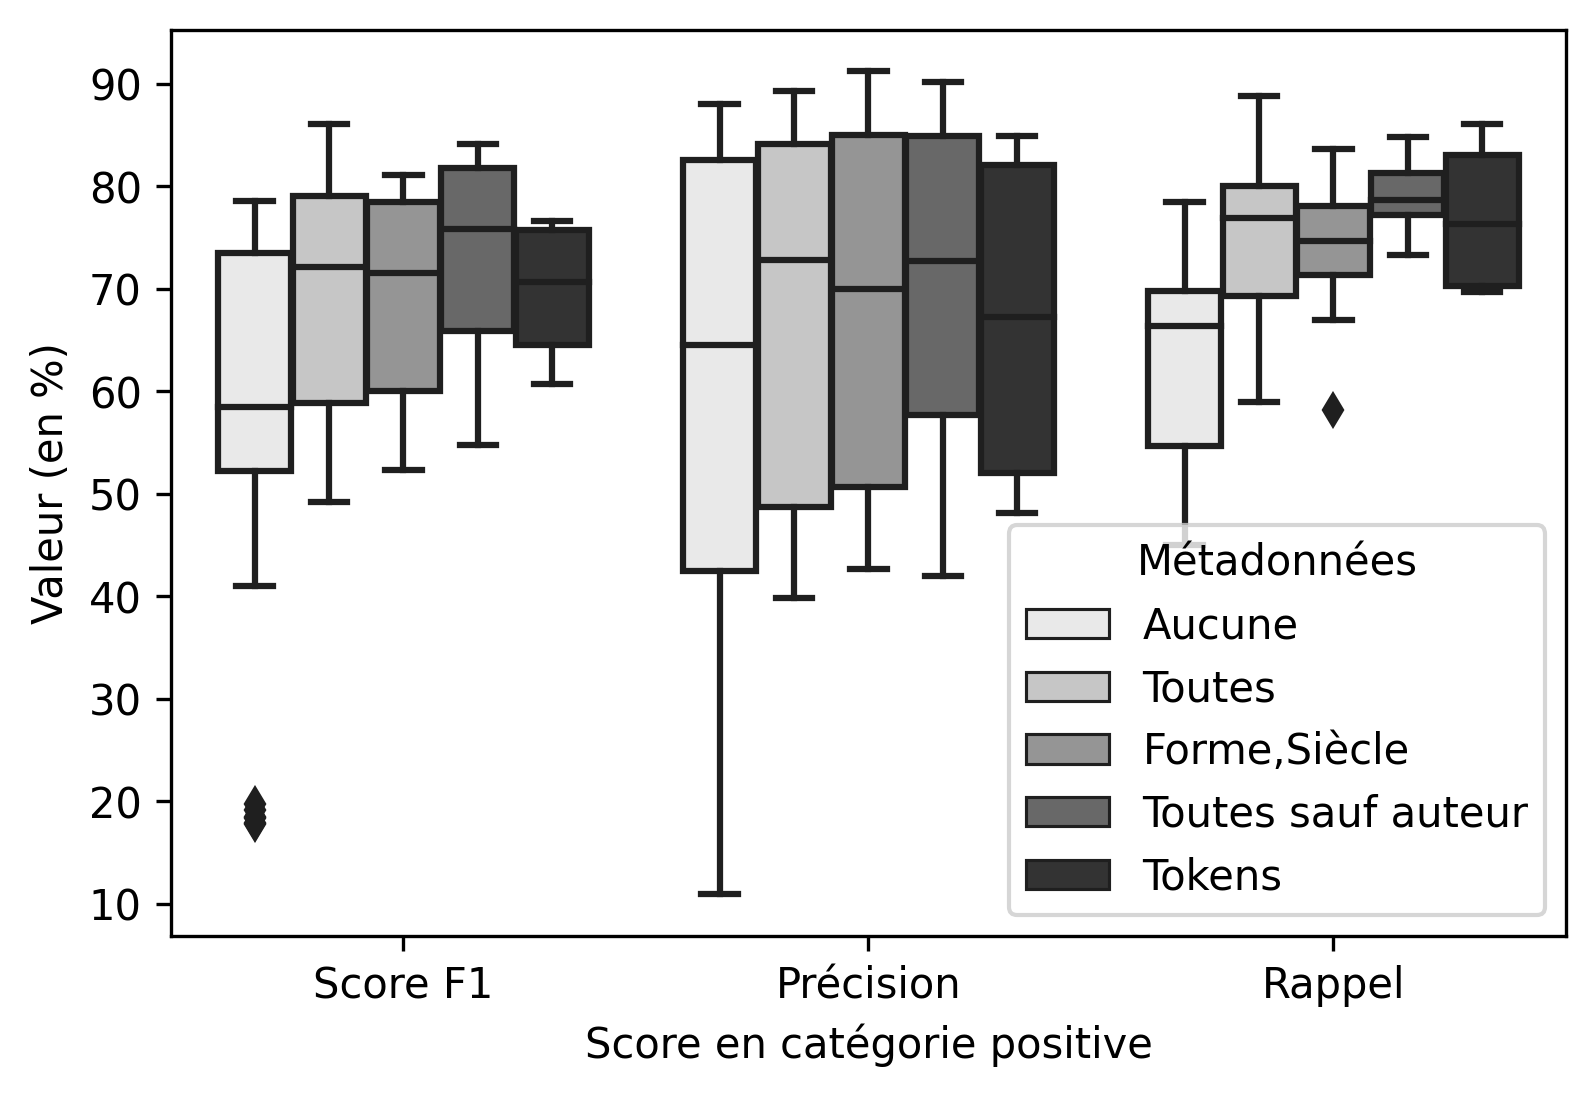
\includegraphics[height=6cm]{figures/chap4/scoreMetadata.png}
    \caption{Dispersion des résultats en fonction des usages de métadonnées (les populations ne sont pas de taille équivalente). On voit une précision sensiblement égale pour les meilleurs modèles de chaque catégorie, plutôt dispersée, tandis que le rappel est peu dispersé dans chacune des catégories mais connait des écarts entre modèles plus forts, avec un net avantage pour les architectures bénéficiant des métadonnées.}
    \label{fig:chap4:metadata-boxplot}
\end{figure}

L'hypothèse de l'efficacité qu'amèneraient les éléments extralinguistiques portés par les métadonnées est confirmée (\textit{cf.} figure \ref{fig:chap4:metadata-boxplot}): sur les cinquante entraînements, en utilisant le score F1 sur la catégorie positive comme mesure de classement, les onze meilleurs utilisent un réseau enrichi de métadonnées, soit au niveau de la couche linéaire soit au niveau du réseau d'encodage LSTM. Avec 86,05\% en score F1, 87,25\% en rappel et 84,88\% en précision sur la catégorie positive, le meilleur des modèles se situe à 4.87 points du score F1 du meilleur modèle n'utilisant pas les métadonnées identifiant les auteurs et structures logiques\footnote{Et à 9,56 points en rappel et à 0,01 en précision, ce qui est négligeable pour ce dernier} (\textit{cf.} table \ref{tab:chap4:resultats-metadata}) . Si on le compare au premier modèle qui n'utilise aucune métadonnée, l'écart se creuse à 8 points de score F1 et 17,13 de rappel. Sur les 25 premiers modèles, 9 utilisent toutes les métadonnées (36\%), 8 utilisent toutes les métadonnées sauf celle identifiant l'auteur (32\%), 7 utilisent les métadonnées Forme et Siècle (28\%), 2 n'en utilisent aucune (8\%, \textit{cf.} table \ref{tab:chap4:metadata-p-value}). Les modèles à métadonnées dépassent donc ceux n'en ayant pas, et l'inclusion de la métadonnée Auteur ou Structure de Citation est plus importante que celles du Siècle ou de la Forme.


\begin{table}[ht]
    \centering
    \resizebox{\textwidth}{!}{%
    \begin{tabular}{llrr}
    \toprule
                   Texte & Métadonnées utilisées        & En tant que Cicéron & En tant que Martial \\
    \midrule
    \textit{De Finibus}, Cicéron & Toutes                       &               4.25\% &              72.60\% \\
    \textit{Épigrammes}, Martial &                              &               7.89\% &              82.05\% \\ \midrule
    \textit{De Finibus}, Cicéron & Toutes sauf Auteur           &               4.69\% &              47.54\% \\
    \textit{Épigrammes}, Martial &                              &               7.33\% &              59.76\% \\ \midrule
    \textit{De Finibus}, Cicéron & Forme et Siècle              &               0.91\% &              36.03\% \\
    \textit{Épigrammes}, Martial &                              &               6.41\% &              48.10\% \\ \midrule
    \textit{De Finibus}, Cicéron & Aucune                       &               2.91\% &               2.91\% \\
    \textit{Épigrammes}, Martial &                              &              15.29\% &              15.29\% \\
    \bottomrule
    \end{tabular}%
    }
    \caption{Nombre de phrases annotées automatiquement comme positives en fonction des modèles avec les meilleurs scores pour chaque type d'usage des métadonnées. L'absence d'usage de métadonnées n'a évidemment aucun impact sur les scores, tandis que l'impact des métadonnées sur le taux de positif est corrélé aux nombres de catégories de métadonnées utilisées.}
    \label{tab:chap4:martial-ciceron}
\end{table}


Cependant, l'application du modèle sur des données hors domaine, sur des données de terrain, réserve une surprise: les modèles de métadonnées avec l'information Auteur et Structure logique de citation ont d'aussi bons scores parce qu'ils ont été victimes d'un surapprentissage dû aux biais inhérents de notre corpus: le modèle reconnaît l'auteur plus qu'il ne reconnaît l'isotopie. Pour prouver ce problème de surapprentissage, on propose l'expérience suivante:
\begin{enumerate}
    \item Le modèle est appliqué sur deux oeuvres: les \textit{Épigrammes} de Martial, connus pour la sexualité qui y est présente, mais pas omniprésente (de nombreux épigrammes si ce n'est la majorité parlent de sujets tout autres); le \textit{De Finibus} de Cicéron, texte philosophique qui ne devrait pas contenir beaucoup de passages présentant l'isotopie sexuelle.
    \item On modifie intentionnellement les métadonnées fournies au modèle: pour chaque texte, on trompe le modèle en alternant entre l'une ou l'autre des identités des textes: les \textit{Épigrammes} sont analysés une fois en tant qu'\textit{Épigrammes}, et une autre fois en tant que \textit{De Finibus}.
    \item Chaque texte est annoté avec le meilleur modèle utilisant: (1) l'ensemble des métadonnées, (2) l'ensemble sauf l'information auteur, (3) les métadonnées Forme et Siècle uniquement, et (4) sans aucune métadonnée (\textit{cf.} table \ref{tab:chap4:resultats-metadata} pour les scores de ces modèles). Les modèles n'utilisant pas de métadonnées ne produisant pas de variation en fonction de ces dernières, les résultats sont le fruit d'une seule prédiction.
    \item On récupère le pourcentage de phrases dont la catégorie prédite par le modèle est Positive.
\end{enumerate}
Le résultat de cette expérience montre un surapprentissage évident sur les métadonnées, décroissant avec le nombre de catégories de ces dernières. Le \textit{De Finibus} annoté comme \textit{Épigrammes} avec l'ensemble des métadonnées (72,60\%) contient vingt-cinq fois plus de phrases positives que celui annoté   par un modèle non enrichi (2,91\%), et près de quatre-vingts fois plus que le modèle Forme+Siècle utilisant l'identité de Cicéron (0,91\%).

L'usage de métadonnées est-il à proscrire ? Si l'on en s'arrête aux résultats, en particulier l'escalade importante qui s'opère sur Martial et Cicéron, la réponse est oui, l'inclusion de métadonnées provoque une bien trop haute variation pour être prise sans risque. Même en pondérant les scores à l'aide de la précision (84,78\% pour le modèle Siècle et Forme), toutes choses égales par ailleurs\footnote{Ce qui est assez peu probable.}, le modèle trouverait 40\% de phrases présentant des traits d'une isotopie sexuelle détectée par le modèle de manière juste. Bien que le corpus présente cette surreprésentation, il sera difficile de faire autrement; les \textit{Épigrammes} seront toujours composés d'un très grand nombre de poèmes à isotopie sexuelle, tandis que Cicéron le sera très rarement, aucune recomposition de corpus ne peut changer cela. Il est dans un sens normal que le modèle soit plus attentif à des tournures particulières chez Martial que chez Cicéron: le lecteur humain sera sûrement aussi en ce sens \enquote{surentraîné} -- on dirait normalement plus attentif -- grâce à sa fine connaissance du corpus et au biais que celle-ci induit. Même en ne prenant en compte que la métadonnée Forme, vu le corpus latin, il est attendu que l'on trouve plus facilement en vers une isotopie de la sexualité qu'en prose. Si l'on prend en compte ce biais, le modèle fonctionne: il prend bien en compte les particularités de chaque trait idiolectal ou sociolectal qu'il identifie.

Outre les modèles à métadonnées, le meilleur modèle non enrichi, même s'il est moins efficace d'après le score obtenu sur le corpus de test, donne des résultats plus crédibles pour Martial et Cicéron avec 2,91\% de phases identifiées positives dans le \textit{De Finibus} et 15,29\% dans les \textit{Épigrammes} (après pondération via la précision sur le corpus de test, toutes choses égales par ailleurs, 2,47\% et 13,01\%). Il reste à choisir ce que l'on préférera: doit-on avoir plus de faux positifs, y compris à cause d'un \enquote{léger} surentraînement, ou doit-on réduire ce bruit au risque de perdre de l'information (le modèle sans métadonnée tombant à 72\% de rappel) ? 

% Nous faisons le pari des faux positifs, toujours dans l'objectif de questionner le texte, de laisser la place au philologue dans la compréhension du texte, tout en lui fournissant un corpus à explorer plus facilement que s'il ne fallait chercher soi-même les centaines de phrases qui pourraient rentrer dans cette catégorie.

\subsubsection{Plongements contextuels de mots}

Les \textit{embeddings} traditionnels (\textit{Word2Vec, GloVe, FastText} entre autres) posent le problème de l'absence de désambiguïsation. Si un travail important a lieu pour essayer d'introduire cette information dans le dictionnaire de vecteurs qu'ils produisent, il ne porte pour l'instant pas ses fruits et s'est fait dépasser par une autre approche: les \textit{embeddings} contextuels, tels \textit{BERT}. En effet, pour reprendre l'exemple de Pedro Javier Ortiz Suárez \textit{et al.}\footcite{ortizsuarez:hal02148693}, pour les outils traditionnels comme \textit{Word2Vec}, \enquote{Washington} représente à la fois l'état, la ville, le président (mais aussi quelques acteurs, îles, etc.). BERT, en produisant des projections en contexte, permet d'outrepasser -- en partie -- ce problème. En utilisant \textit{Latin BERT}\footcite{bamman2020latin} comme entrée seule ou comme complément à la phrase encodée, nous proposions d'évaluer les capacités de BERT dans un objectif de classification.

\begin{figure}[t]
    \centering
    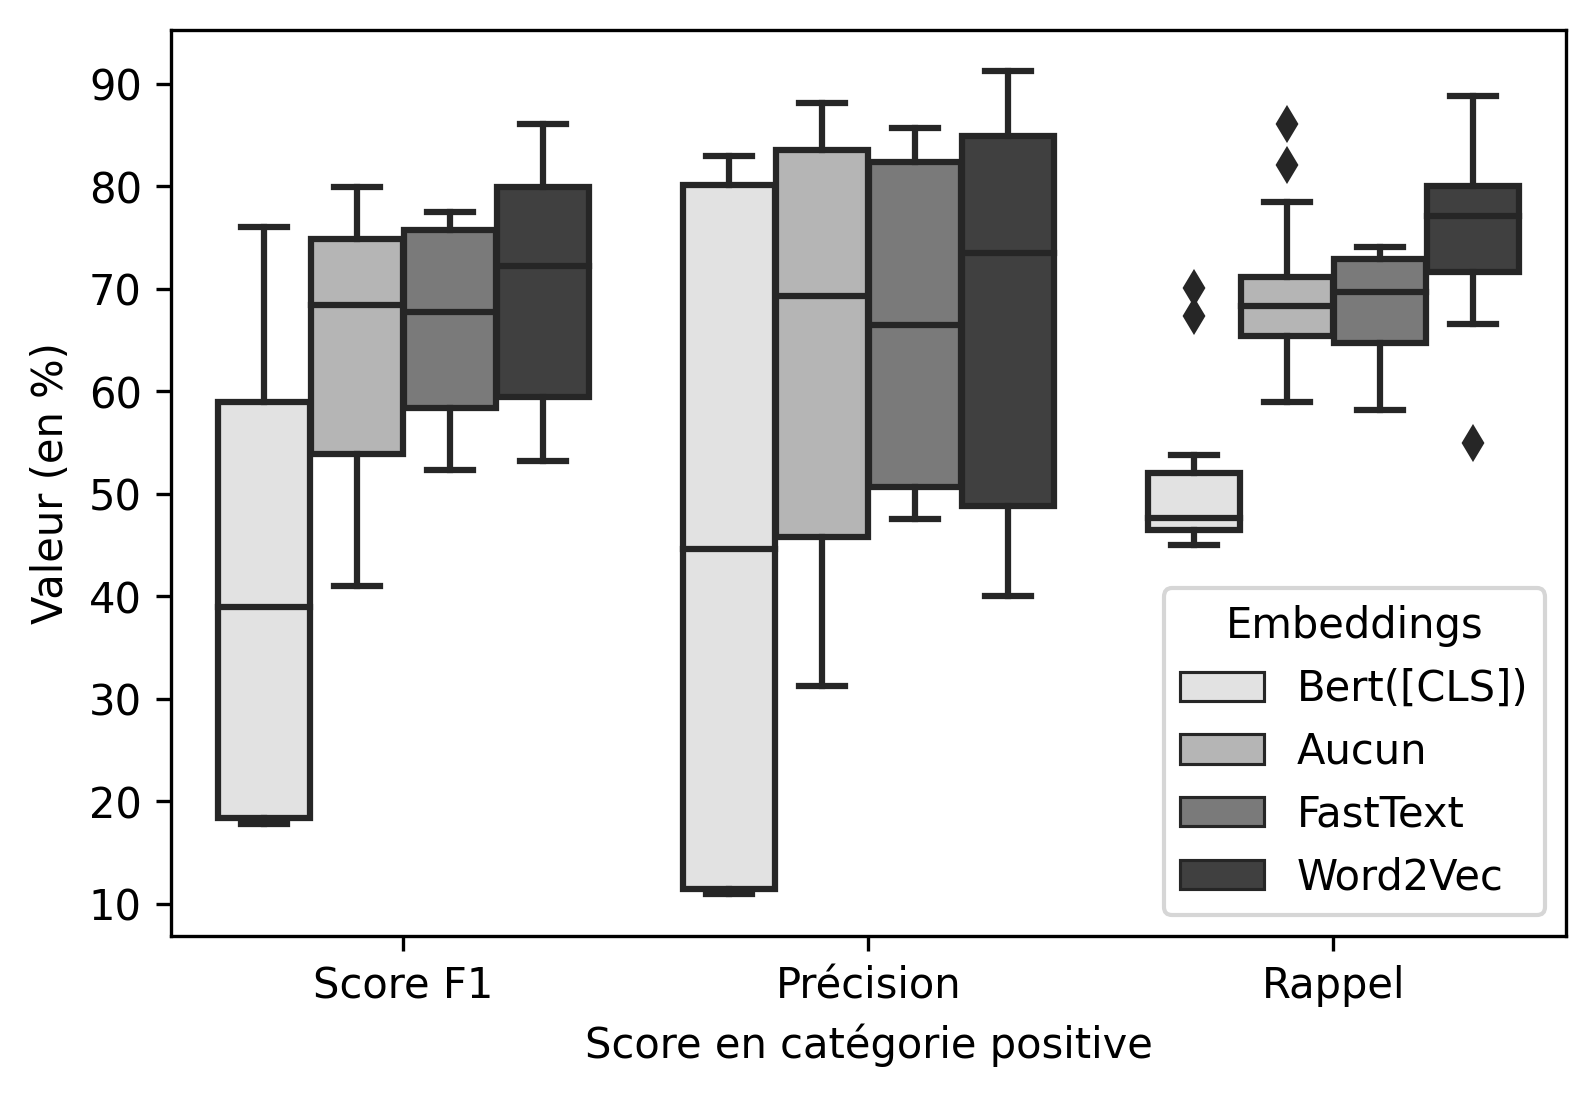
\includegraphics[height=6cm]{figures/chap4/scoreDispersionEmbeddings.png}
    \caption{Dispersion des résultats en fonction du système d'\textit{embeddings} utilisé. BERT est utilisé ici comme source  d'information supplémentaire, et non comme source unique, via un \textit{pool} du token \texttt{[CLS]} en dernière couche d'encodage.}
    \label{fig:chap4:bert-dispersion-fusion}
\end{figure}

Le résultat est clair: \textit{Latin BERT} n'apporte pas de bénéfices importants en tant que complément d'information, voire enregistre des sous-performances face aux autres modèles (\textit{cf.} figure \ref{fig:chap4:bert-dispersion-fusion}). Le premier modèle mixte \texttt{HAN(Lemme)+BERT->Linéaire} se place en 36e position du classement original avec un score F1 de 76,02\%, un rappel de 70,11\% et 83,01\% de précision, à 2 points du premier modèle n'utilisant pas BERT. La puissance de calcul demandée part BERT étant importante, si ses performances ne sont pas compétitives avec un modèle "traditionnel", il n'y a pas d'intérêt à le conserver. Non affichée dans les résultats, une tentative de ré-entraînement de BERT pour le spécialiser (anglais \textit{fine tune}) sur le dataset bloquait les résultats sous la barre des 20\%, probablement à cause de la très petite taille des données\footnote{Un problème d'implémentation ne peut être exclu.}.

\afterpage{%

\begin{sidewaysfigure}
    \begin{subfigure}{0.48\hsize}
        \centering
        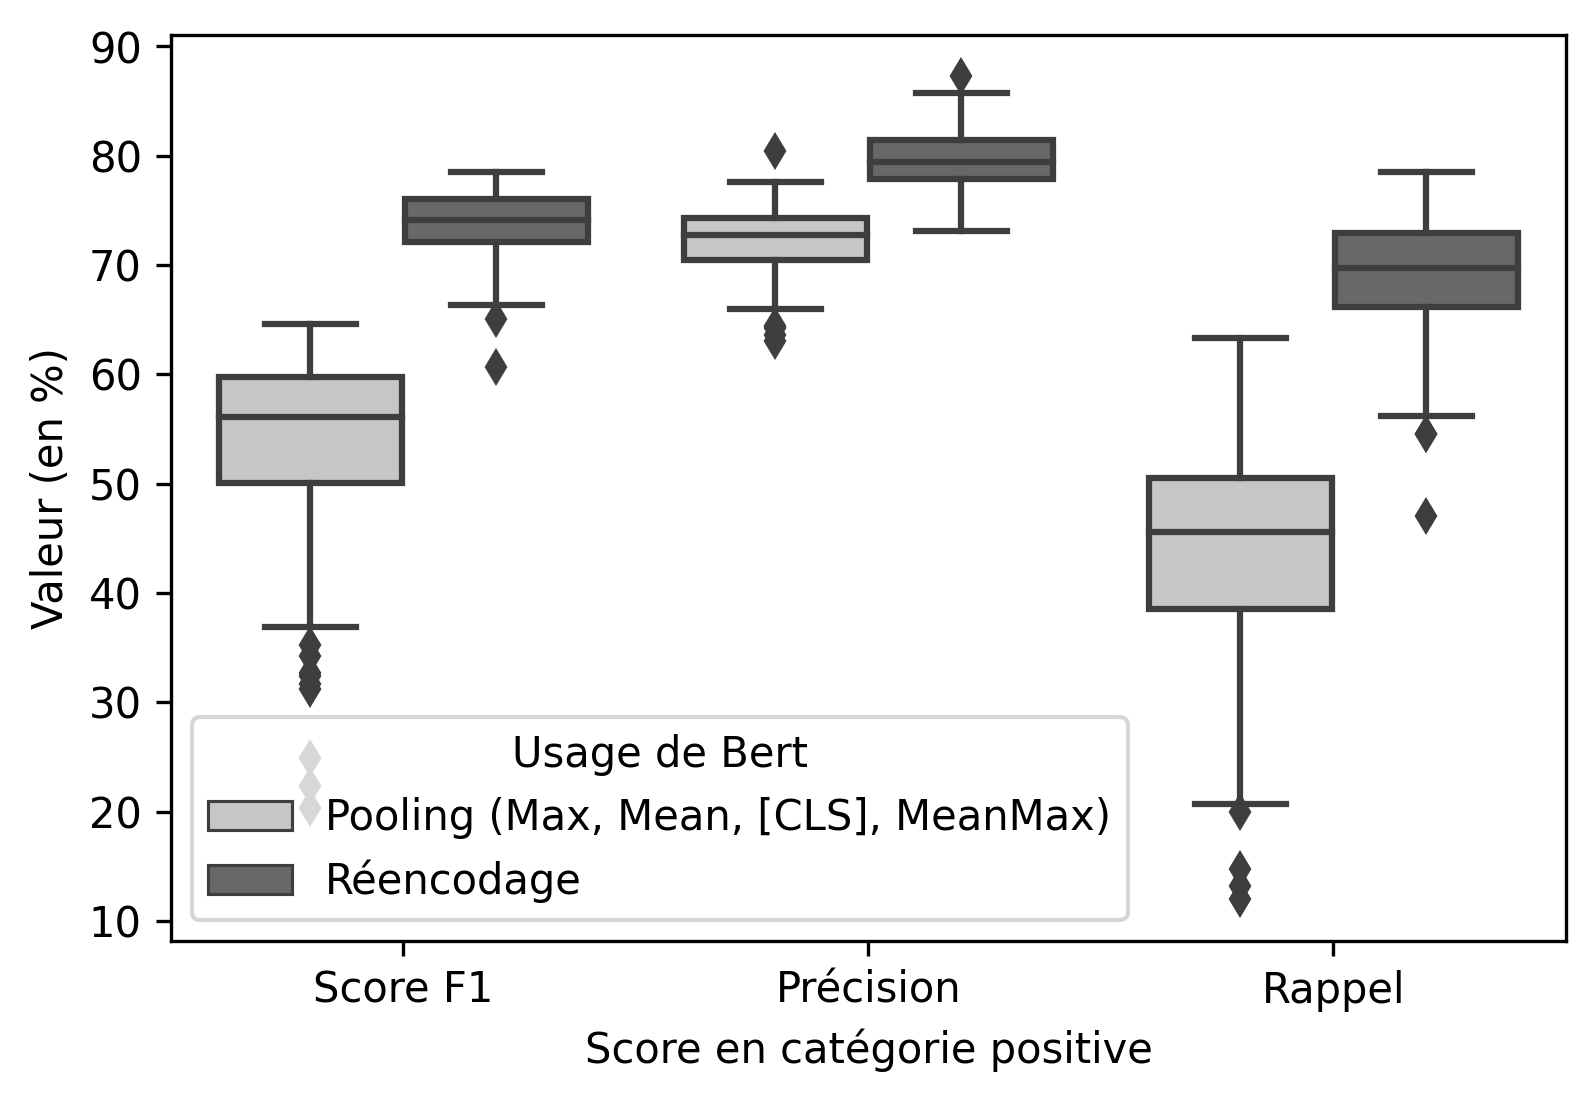
\includegraphics[width=0.9\hsize]{figures/chap4/BertPoolingGeneric.png}
        \caption{Dispersion des résultats en fonction des catégories de méthodes d'exploitation des encodages BERT: \textit{Pooling} contient les méthodes \texttt{MeanMax}, \texttt{Max}, \texttt{Mean} et l'usage du token \texttt{[CLS]}}
        \label{fig:chap4:bert-pooling-generic-eval}
    \end{subfigure}%
    \hfill%
    \begin{subfigure}{0.48\hsize}
        \centering
        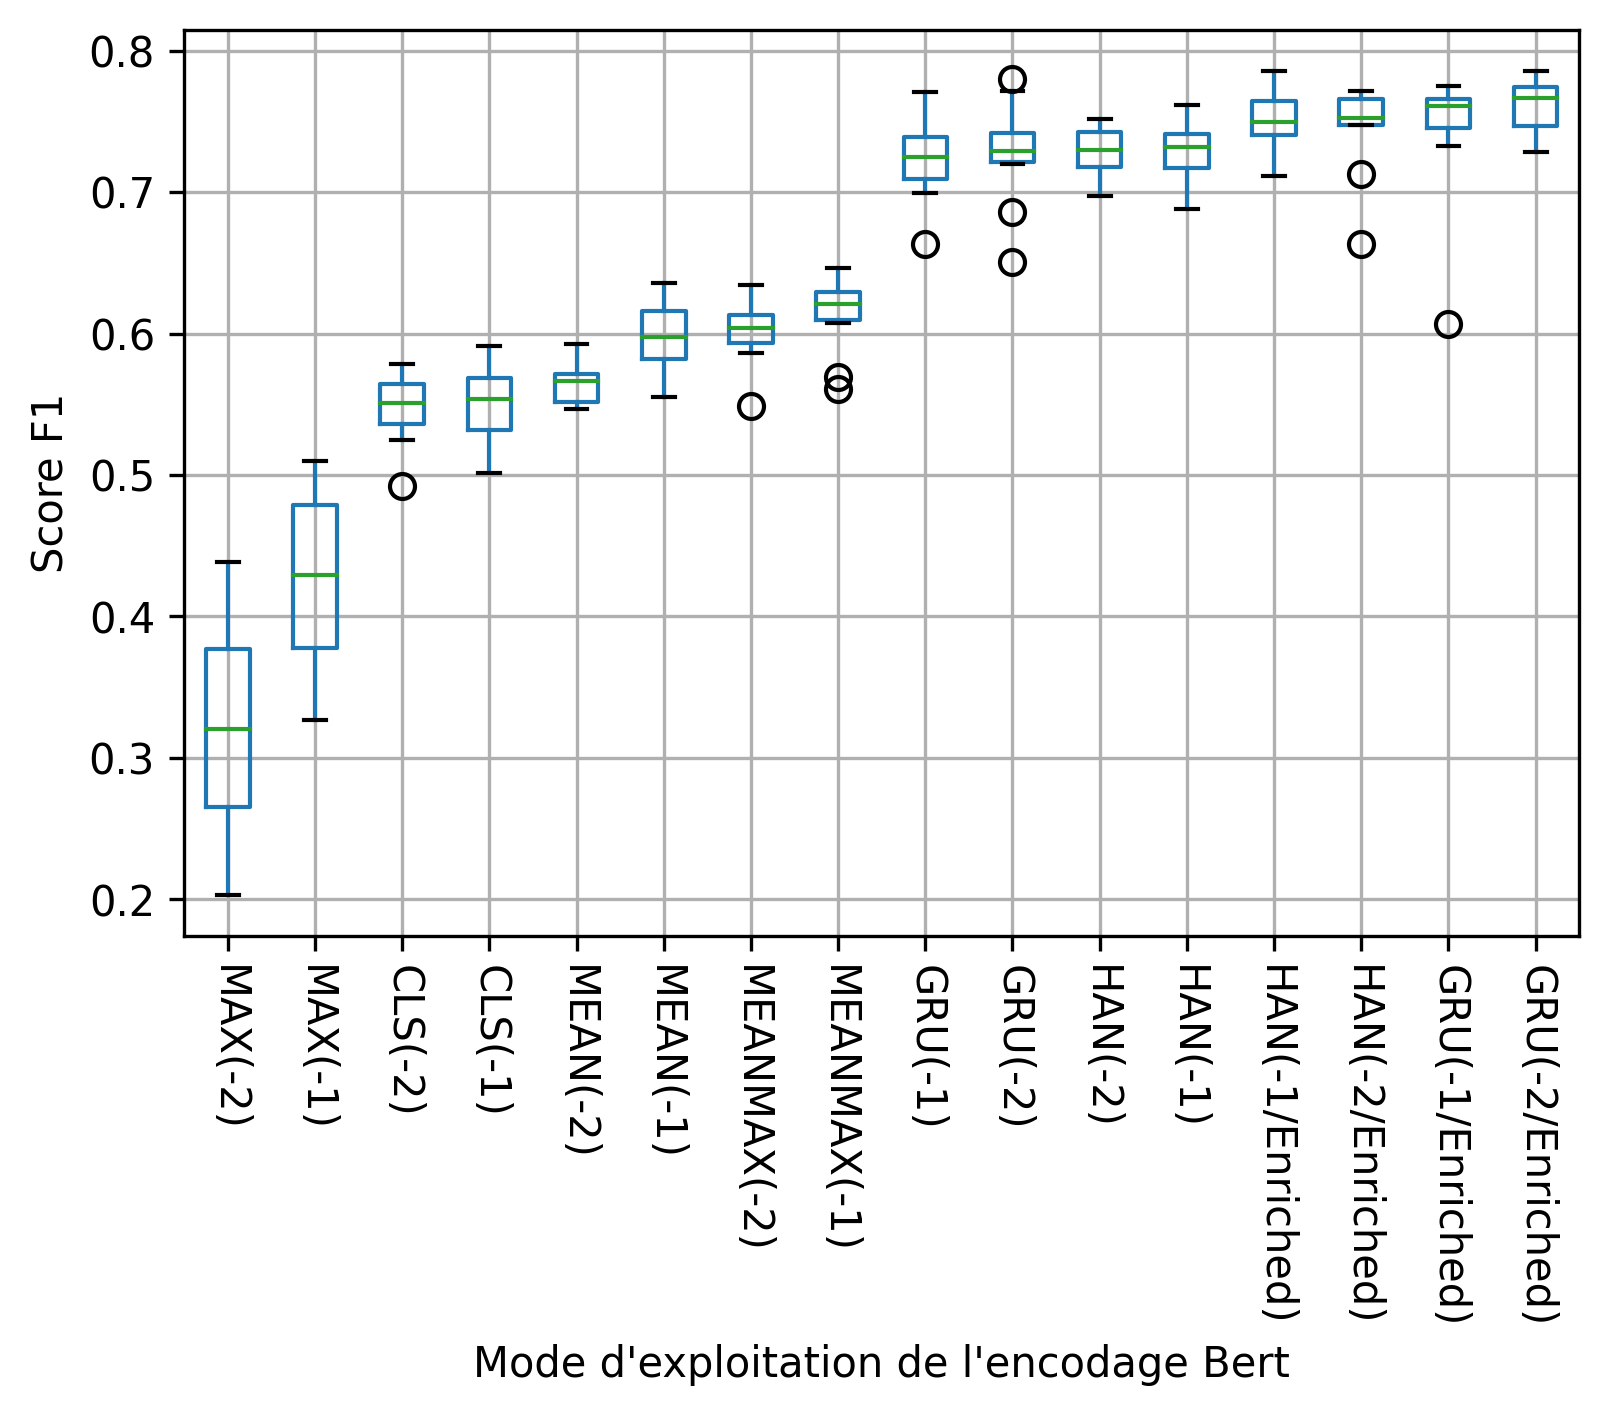
\includegraphics[width=0.9\hsize]{figures/chap4/BertPoolingDetailed.png}
        \caption{Dispersion des résultats en fonction de la méthode d'exploitation des encodages BERT et de la couche (entre parenthèse) utilisée (-1 étant la dernière couche, -2 l'avant-dernière). Les méthodes de ré-encodages sont les plus performantes, la couche utilisée ayant peu d'effet sur les résultats. Chaque architecture est entraînée 10 fois, avec une couche linéaire comme couche décisionnelle.}
        \label{fig:chap4:bert-pooling-detailed-eval-fscore}
    \end{subfigure}%
    \caption{Étude des dispersions des résultats des modèles utilisant BERT dans leur architecture.}
\end{sidewaysfigure}
\clearpage
}
Pour ce qui est des architectures reposant sur BERT, sans affinage, celles utilisant une couche d'encodage de type GRU ou HAN fournit des résultats plus convaincants (\textit{c.f.} figure \ref{fig:chap4:bert-pooling-generic-eval}). Les méthodes mentionnées plus tôt en \ref{part:chap4:architectures:variations-architectures:encodage} n'ont pas nécessairement amélioré les résultats face à un usage classique du token \texttt{[CLS]}, mais induisent cependant bien des variations. Là où le \textit{pooling} du token \texttt{[CLS]} est nécessairement dans les 4 plus mauvais modèles en score F1, précision et rappel, la sélection par la valeur maximum (\texttt{Max}) ou par concaténation de la valeur maximum et de la moyenne (\texttt{MeanMax}) sont régulièrement dans le top 4 des modèles à \textit{pooling}. Mais ces architectures n'en restent pas moins très très loin des modèles à ré-encodage, presque 20 points entre les médianes de score F1 des deux catégories d'usage de BERT, avec un maximum pour le \textit{pooling} qui touche à peine le bas de la moustache inférieure des méthodes GRU et HAN.

En général, les encodages des projections BERT par HAN et GRU, potentiellement suivis d'une couche linéaire enrichie, touchent les résultats en Score F1 du meilleur modèle sans métadonnées. L'enrichissement par métadonnées influent clairement les résultats de plusieurs points et inversent même l'intérêt des modèles (HAN est meilleur que GRU sans métadonnées, mais cède sa place de premier avec). GRU montre de très bons résultats dans son premier quartile, à égalité avec les modèles enrichis. Bien que les scores soient largement meilleurs comparés aux modèles \texttt{[CLS]} présentés plus haut, ils restent au niveau d'architectures plus traditionnelles, pour un coût plus élevé en entraînement et calcul d'inférence.

\subsubsection{L’échec des modèles de similarité}

\begin{figure}[p]
    \centering
    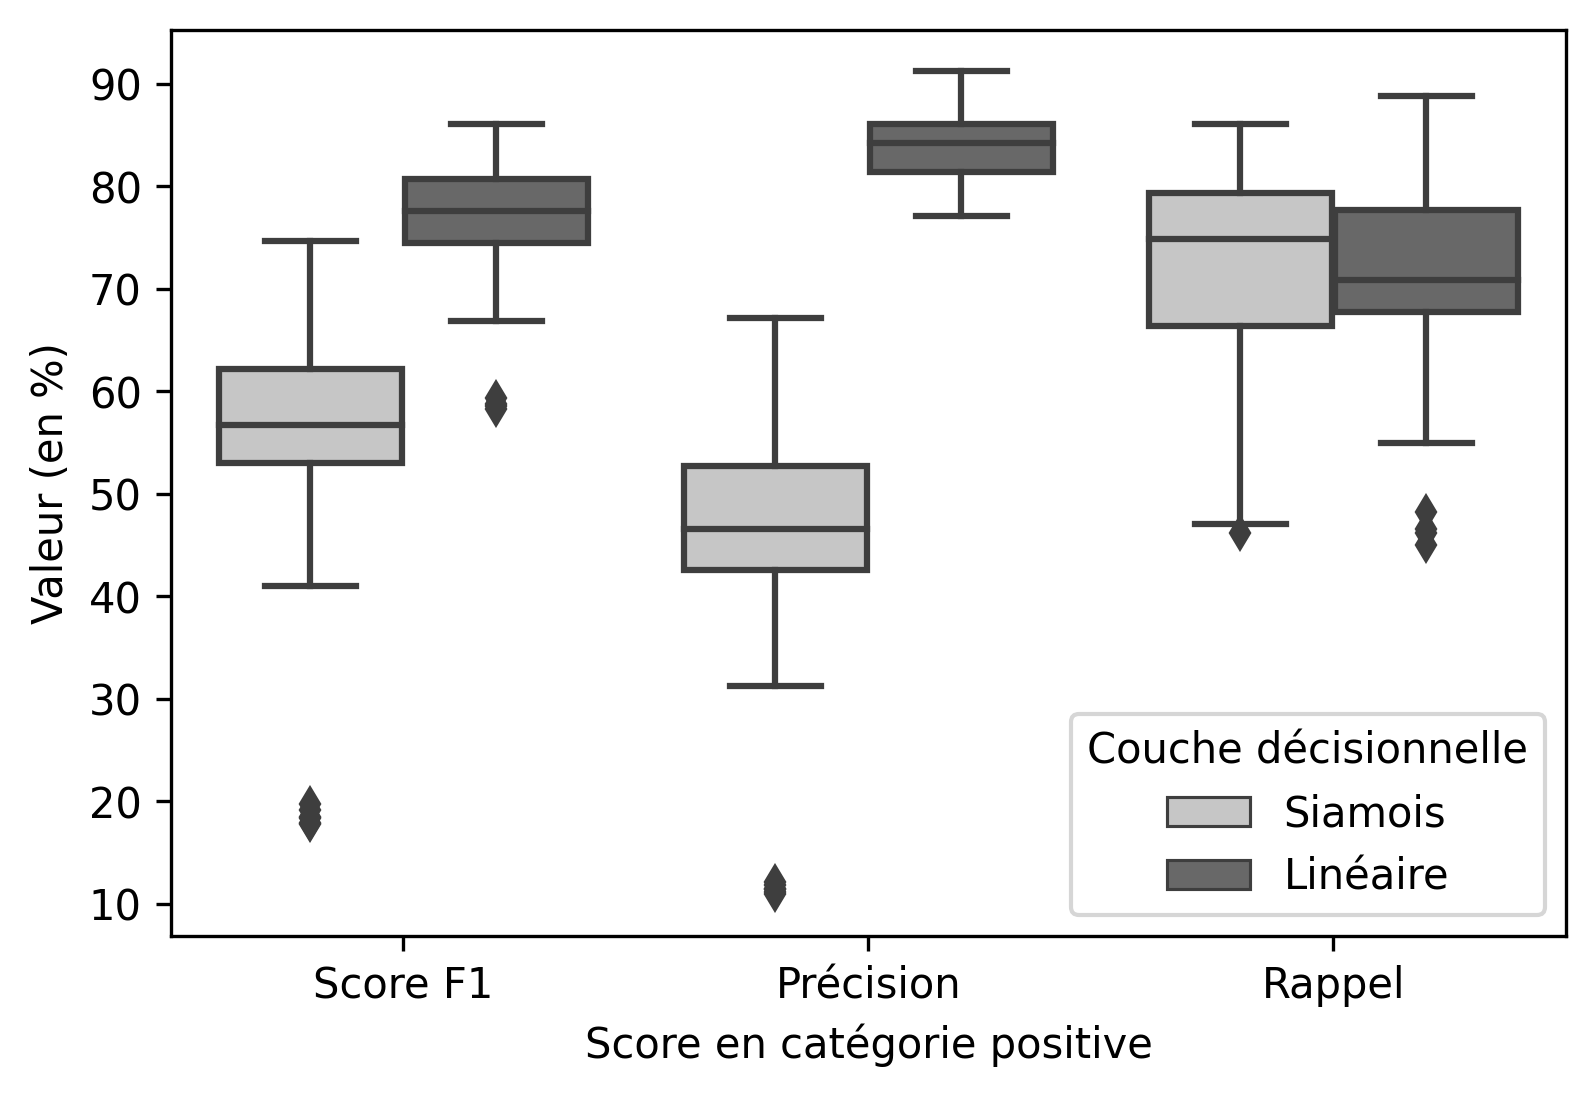
\includegraphics{figures/chap4/SiameseVsLinear.png}
    \caption{Dispersion des résultats, à population quasi égale, entre les modèles à couche linéaire et à couche de similarité. En dehors du rappel (proportion de réponses sûres parmi les réponses fournies), les modèles à couche de similarité sont largement dépassés par les modèles linéaires sur les autres éléments de mesure.}
    \label{fig:chap4:modeles-siamois-vs-lineaires}
\end{figure}

Nous avions proposé en type d'architecture de faire varier les couches décisionnelles entre couche de réseaux siamois et couche en réseau linéaire, les réseaux siamois étant vantés par la littérature scientifique comme particulièrement adaptés pour les petits stocks de données. Les résultats présentés \ref{fig:chap4:modeles-siamois-vs-lineaires} ne reprennent que les modèles utilisant une couche en \textit{constrastive loss} et montrent qu'ils ne sont pas à la hauteur de nos attentes.

Seuls les modèles en \textit{constrastive loss} sont présentés dans le tableau final de résultats \ref{tab:chap4:general-results}, mais toutes les variations suivantes ont été utilisées, sans provoquer de différence nette avec la configuration incluse dans les schémas:
\begin{itemize}
    \item les configurations en \textit{triplet loss} n'apportaient aucun bénéfice. La comparaison avec un exemple positif et un exemple négatif ou la comparaison avec un seul exemple positif ne change pas les résultats du modèle.
    \item Les techniques d'échantillonnage mentionnées plus haut -- \textit{BatchEasyHard} \footcite{xuan_improved_2020} et \textit{BatchHard}\footcite{hermans_defense_2017} -- n'ont pas modifié les résultats non plus. Ces deux méthodes cherchent à sélectionner les exemples les plus difficiles à différencier ou à classer ensemble dans un batch.
    \item Nous avons utilisé une  variation de \textit{BatchEasyHard} dans laquelle tous les documents sont comparés à l'ensemble des autres documents d'un même batch. Cette méthode n'a pas amélioré les résultats.
\end{itemize}

Les résultats sont donc peu probants et posent légitimement la question de la source de cette \enquote{déception}. En dehors d'une possible -- mais peu probable au vu du nombre de tests -- erreur d'implémentation, il reste l'hypothèse de l'inadéquation des modèles siamois pour ce type de tâche, reposant sur des textes extrêmement courts avec une très forte disparité lexicale entre les différents éléments. En effet, la plupart des cas utilisant les réseaux en comparaison cherchent à sélectionner des éléments qui présentent de fortes similarités, graphiques ou textuelles: peu de variations existent entre un filigrane et un autre; une annonce de vente pour un téléphone portable est proche de celle d'un autre de la même marque et utilisent probablement des informations et lexiques similaires. À la surface, nos textes sont différents, et le modèle n'est pas capable de comprendre suffisamment bien leur similarité sous-jacente. Une autre hypothèse: les modèles ne restent pas catastrophiques (50\% de précision environ, soit 50\% de faux positifs parmi ceux trouvés) et pourraient très bien être plus résistants sur des données nouvelles: si l'on regarde les résultats des modèles à métadonnées et leur 36\% de contenus \enquote{sexuels} dans les \textit{Épigrammes}, il n'est pas improbable que de nombreux résultats parmi eux soient de faux positifs, plus que le taux de 75\% le promet en tout cas.

\subsubsection{Architectures des meilleurs modèles}

D'après les premiers résultats (table \ref{tab:chap4:general-results}), les modèles présentant les meilleurs résultats sont ceux:
\begin{itemize}
    \item incluant les métadonnées dans leur couche d'encodage (LSTM) ou de décision (Linéaire);
    \item incluant ou non l'information morphologique;
    \item avec une couche de décision linéaire
    \item utilisant un encodeur LSTM ou un réseau avec attention (HAN).
\end{itemize}

Ces résultats sont confirmés par la seconde phase d'entraînements qui montre un net avantage aux 4 modèles principaux sélectionnés (en premiers sur la table \ref{tab:chap4:general-results}). L'enrichissement en métadonnées, même limitées à l'information formelle et celle du siècle d'appartenance de l'auteur, permet au modèle de mieux analyser les résultats. Mais l'on peut apercevoir aussi que certains modèles, bien qu'éloignés par leur médiane du top 4, peuvent rivaliser: le modèle utilisant HAN et Word2Vec sans enrichissement vient ainsi battre trois des meilleurs modèles en précision, un modèle en GRU et Word2Vec vient battre en rappel les valeurs maximales du top 4 aussi. Il est donc possible de se reposer sur des modèles moins surentraînés, potentiellement aussi capables que des modèles enrichis, avec une perte en test de 1,80 à 4 points suivant les mesures.

Parmi les types de modèles, seuls sont à proscrire les modèles BERT, dont l'entraînement et l'usage en terrain réel sont coûteux et dont les scores sont bien éloignés du top 4, et les réseaux utilisant CNN comme encodeurs, du moins avec des filtres $[2,3,4,5]$ (\textit{cf.} figure \ref{fig:chap4:main-results-dispersion-encoder}). Au contraire, les réseaux utilisant des encodeurs LSTM, GRU ou HAN ont tendance à avoir des résultats équivalents entre eux, avec une dispersion équivalente des résultats. Parmi les paramètres, la taille de la dimension d'encodage n'a pas ou peu d'impact sur les résultats (figure \ref{fig:chap4:main-results-dispersion-dimension}). Il reste que chaque modèle ou type d'architecture présente une forte dispersion de leurs résultats, hors Score F1 (5 points sur le F1 pour les meilleures architectures, mais de 10 à 15 points sur les deux autres mesures): une modification du \textit{learning rate} n'affecte pas cette disparité en précision et rappel. La taille du corpus de test peut être à la source de cette variance.

\noindent\begin{minipage}{\linewidth}
    \centering
    \resizebox{\textwidth}{!}{%
    \begin{tabular}{r|lllll|rrr}
    \toprule
     Index & Morphologie & Encodeur & Enrichissement & Embeddings & Taille encodée &  Précision &  Rappel &  Score F1 \\
    \midrule
        17 &             &      HAN &         Linear &   Word2Vec &            128 &      \textbf{86.86} &   \textbf{75.50} &     \textbf{80.07} \\
        16 &             &     LSTM &           LSTM &   Word2Vec &            256 &      84.28 &   75.10 &     79.53 \\
        15 &  Agglomérée &      HAN &         Linear &   Word2Vec &            256 &      83.38 &   75.30 &     79.51 \\
        14 &  Agglomérée &     LSTM &           LSTM &   Word2Vec &            128 &      85.72 &   72.71 &     78.51 \\
        13 &  Agglomérée &      GRU &                &   Word2Vec &            128 &      \textbf{85.07} &   71.12 &     \textbf{77.22} \\
        12 &  Agglomérée &      HAN &                &   Word2Vec &            128 &      82.38 &   \textbf{71.51} &     76.54 \\
        11 &  Agglomérée &      HAN &                &   Word2Vec &            256 &      84.51 &   69.52 &     76.50 \\
        10 &  Agglomérée &      GRU &                &   Word2Vec &            256 &      84.26 &   69.72 &     76.47 \\
         9 &             &      GRU &         Linear &       BERT &            256 &      80.47 &   70.72 &     76.11 \\
         8 &             &      HAN &         Linear &       BERT &            256 &      82.34 &   69.52 &     74.94 \\
         7 &  Agglomérée &     LSTM &                &   Word2Vec &            128 &      81.80 &   70.72 &     74.57 \\
         6 &  Agglomérée &     LSTM &                &   Word2Vec &            256 &      79.55 &   70.12 &     74.31 \\
         5 &             &      HAN &                &       BERT &            256 &      77.97 &   70.12 &     73.15 \\
         4 &             &      GRU &                &       BERT &            256 &      79.41 &   67.73 &     72.50 \\
         3 &  Agglomérée &      CNN &                &   Word2Vec &            128 &      82.20 &   55.78 &     66.50 \\
         2 &             &  MeanMax &                &       BERT &            256 &      71.63 &   54.58 &     62.07 \\
         1 &  Agglomérée &      CNN &                &   Word2Vec &            256 &      84.65 &   45.62 &     59.90 \\
    \bottomrule
    \end{tabular}%
    }
    \captionof{table}{Score médian des meilleurs modèles, des modèles BERT et de modèles simples (CNN, GRU, HAN, LSTM sans enrichissements) sur 10 entraînements. En gras, les meilleurs scores des modèles avec enrichissement et sans enrichissement. L'enrichissement apporte un réel bonus (+2,8 points en Score F1, +4,40 en rappel, +1,80 en précision), contrairement à l'usage de modèles \enquote{riches} et \enquote{lourds} comme BERT, à la traîne, 1 points environ des meilleurs modèles sans enrichissements.}
    \label{tab:chap4:general-results}
    
    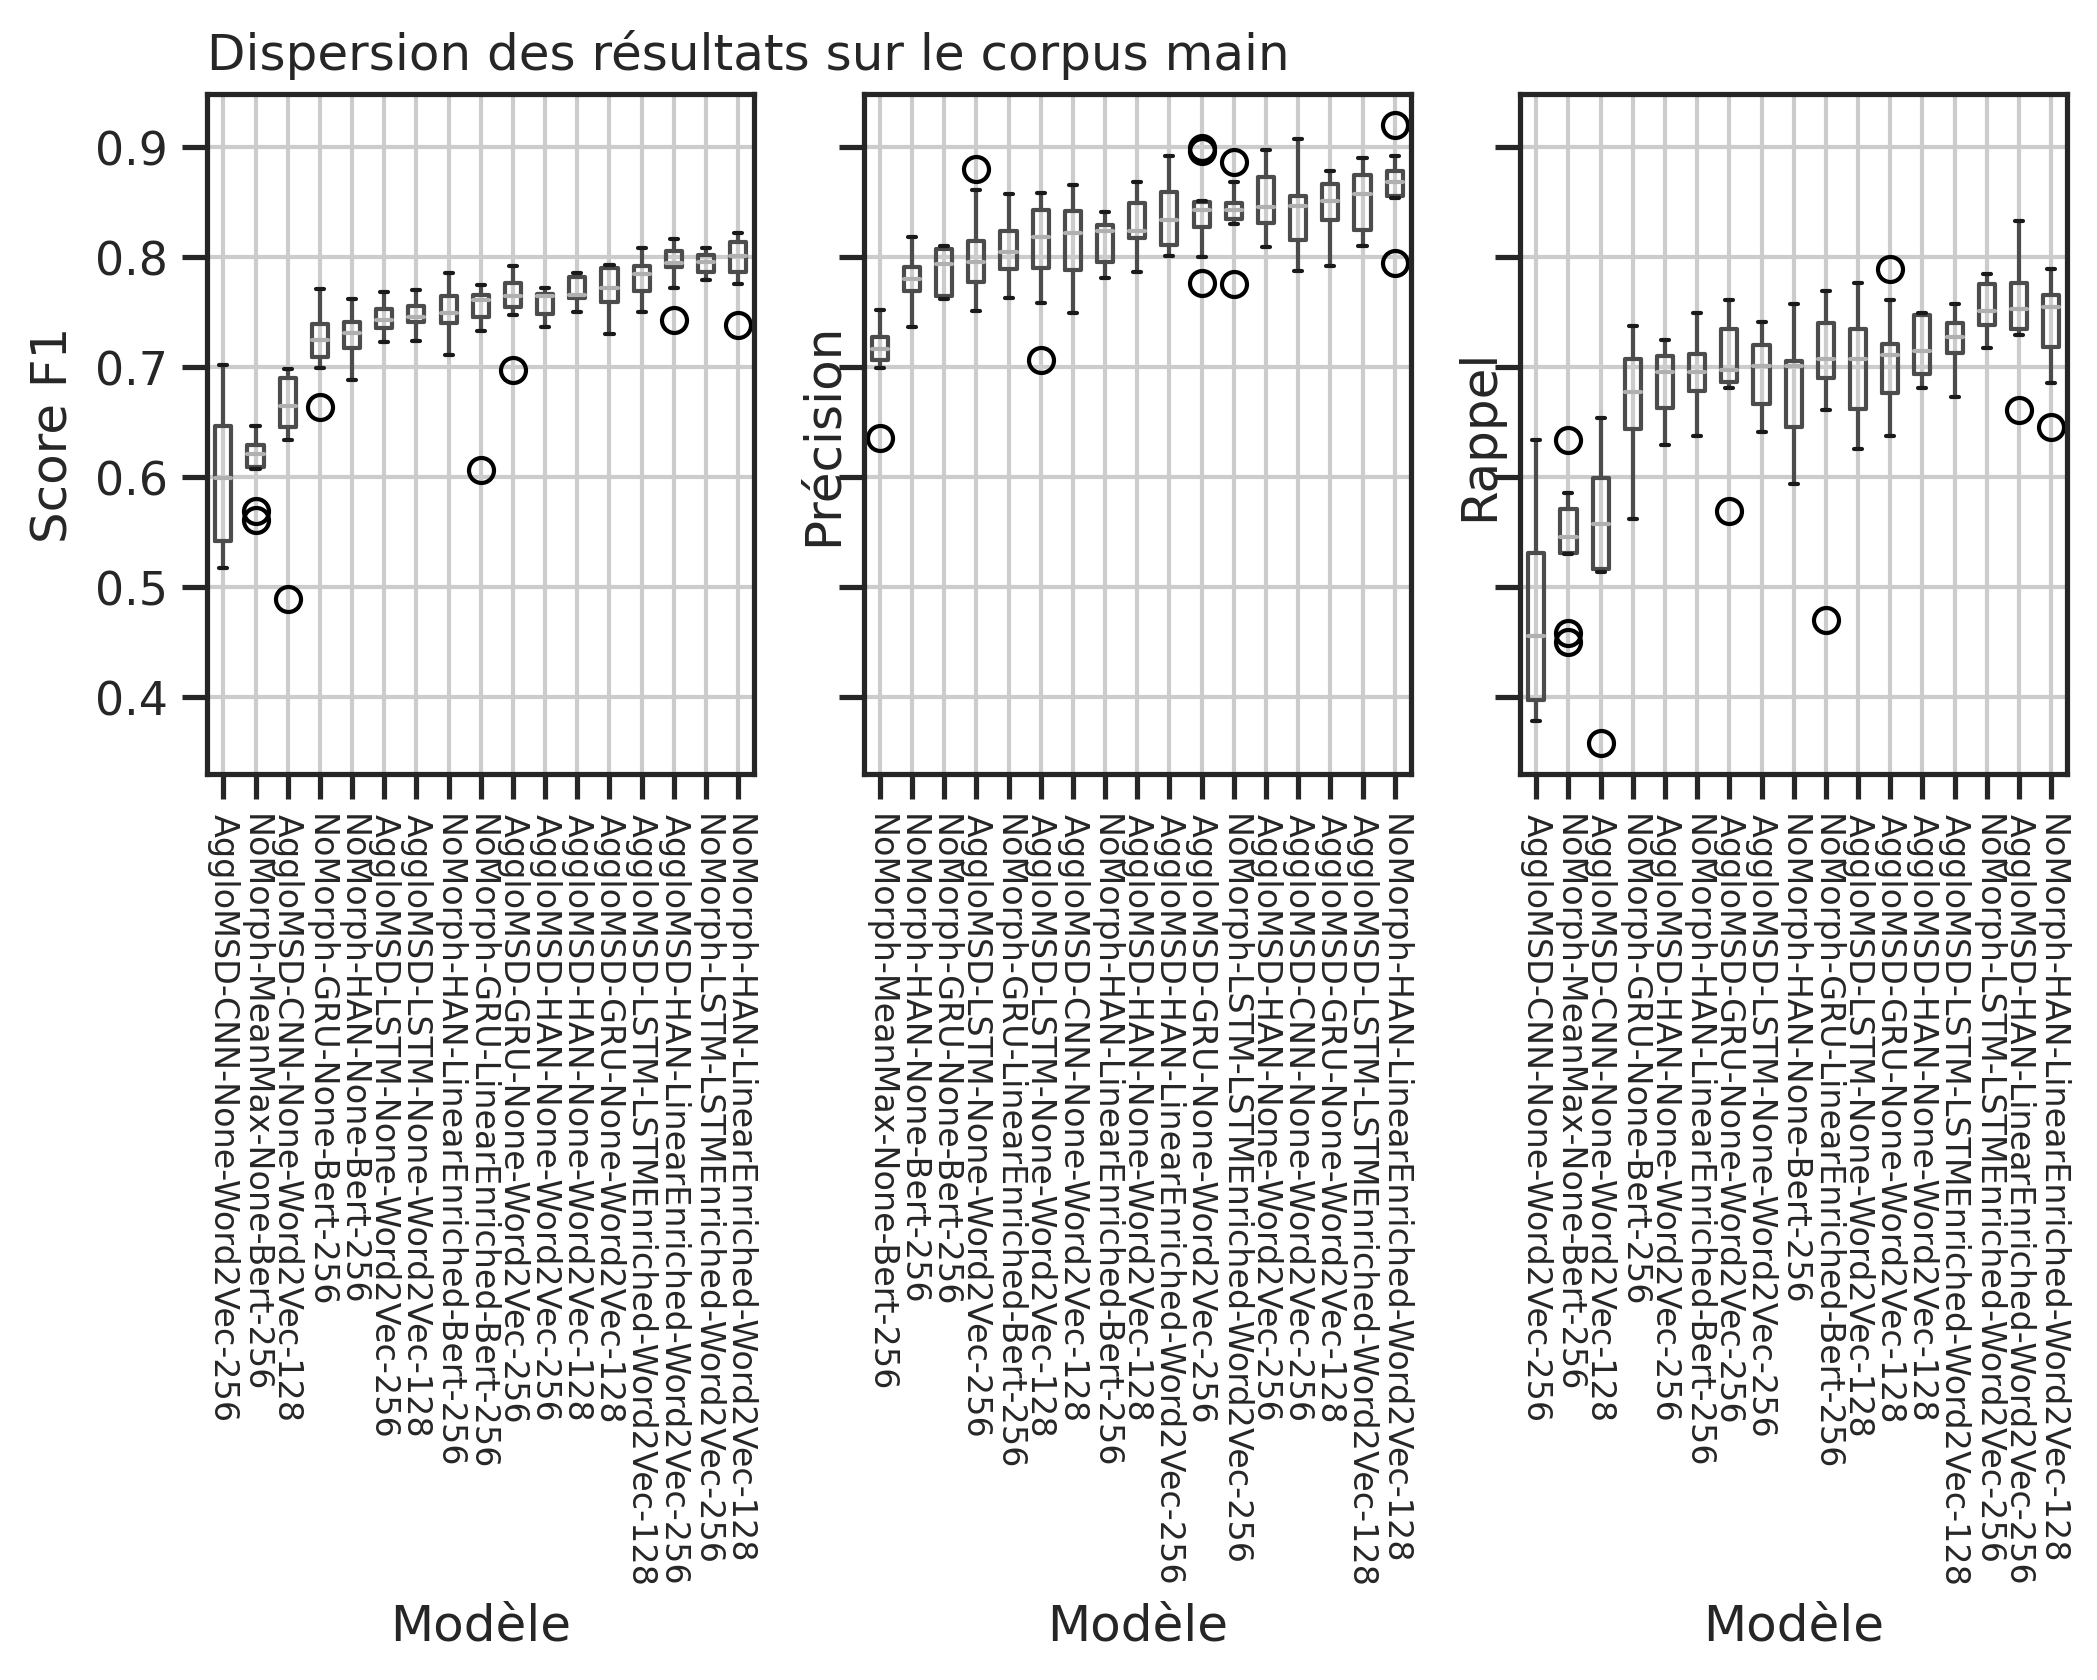
\includegraphics[width=\linewidth]{figures/chap4/main-dispersionscores.png}
    \captionof{figure}{Dispersion des score des meilleurs modèles, des modèles BERT et de modèles simples (CNN, GRU, HAN, LSTM sans enrichissements) sur 10 entraînements. Les détails sur les architectures sont donnés en table \ref{tab:chap4:general-results}}
    \label{fig:chap4:main-results-dispersion}
\end{minipage}

\begin{figure}[ht]
        \begin{subfigure}{0.65\textwidth}
            \centering
            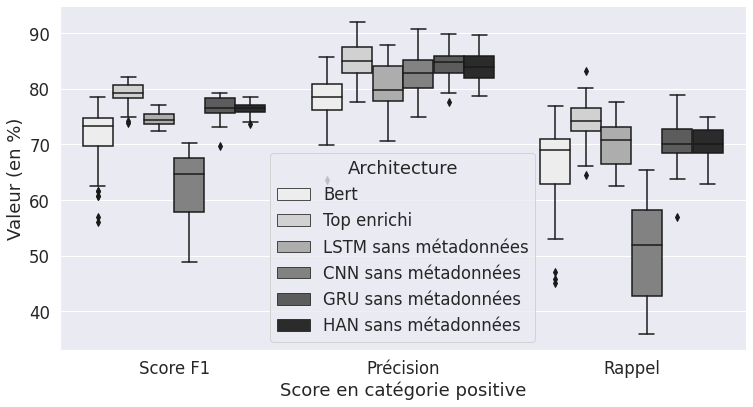
\includegraphics[width=\linewidth]{figures/chap4/main-lineartop5vstheworld.png}
            \caption{Dispersion des scores en fonction des types de modèles (Enrichis, BERT, Classiques) (à gauche) et en fonction des tailles d'encodage (à droite)}
            \label{fig:chap4:main-results-dispersion-encoder}
        \end{subfigure} \hfill %
        \begin{subfigure}{0.30\linewidth}%
            \centering
            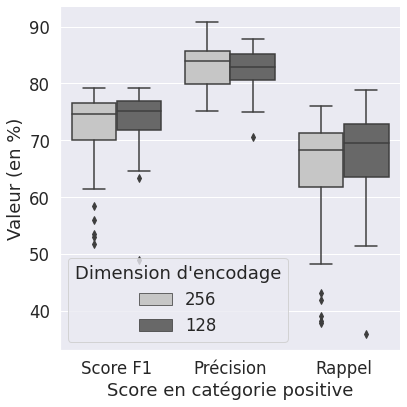
\includegraphics[width=\linewidth]{figures/chap4/main-encodingdimension.png}
            \caption{Dispersion des scores en fonction de la dimension d'encodage, toutes architectures confondues.}
            \label{fig:chap4:main-results-dispersion-dimension}
        \end{subfigure}
        \caption{Dispersion des résultats au niveau macro et non au niveau architecture.}
\end{figure}%
    \clearpage

\subsection{Extensibilité des modèles}

Notre recherche est nourrie de celle de J. N. Adams: non seulement nous n'avons pas eu à chercher les exemples présentant l'isotopie sexuelle manuellement -- car l'auteur nous les avait relevé pour nous -- mais en plus nous avons bénéficié d'un travail de catégorisation de ces dernières. Cette recherche, publiée en 1983, ne connaît que peu d'équivalents dans les littératures latines classiques et tardives. En terme d'autorité, le travail de J. N. André sur les couleurs fait probablement autant référence dans son propre domaine, mais il n'a pas été réimprimé depuis 1949\footcite{andre1949etude}. Il existe ensuite quelques travaux de thèse\footnote{Le travail de Pedro Duarte semble rentrer dans cette catégorie. \textcite{duarte_vocabulaire_2010}} et des articles sur des coupes temporelles ou des parties de lexique plus restreintes. Quoiqu'il en soit, ces travaux, ou de nouveaux à venir, passent par une première compilation qui pourrait être simplifiée. Or, qu'il s'agisse de lexicographie, de stylistique ou bien même d'anthropologie historique, le premier obstacle à cette recherche est celui de la compilation d'exemples dans un corpus de plusieurs dizaines -- voire centaines suivant les bornes choisies -- de millions de mots.

Dans ce cadre, l'expérience de notre recherche peut fournir un outillage à la compilation de ces futurs corpus. Il faut alors pouvoir enquêter sur les limites de cet outillage, dans d'autres conditions. Avec pour seule source notre corpus, il est possible d'évaluer l'efficacité des différents modèles en fonction d'autres versions de ce corpus, en quantifiant l'impact qu'ont par exemple la diversité lexicale, la diversité des exemples ou le nombre de ces derniers. Nous proposons donc trois terrains d'explorations différents, permettant d'évaluer l'apport des différentes architectures:

\begin{enumerate}
    \item Explorer, avec un corpus diversifié en sources, l'importance de sa taille. Avec un corpus beaucoup plus petit, mais comportant une variété d'exemples (avec des métaphores, des termes \enquote{explicitement} liés à l'isotopie, etc.) plus importante.
    \item Étudier la capacité du modèle à reconnaître des termes explicites à partir du simple apprentissage d'exemples \enquote{métaphoriques}.
    \item Étudier la capacité du modèle à reconnaître des exemples métaphoriques en ayant été entraîner sur des exemples ne présentant pas cette figure de style (d'après l'analyse d'Adams).
\end{enumerate}

\begin{table}[]
    \centering
    \begin{tabular}{ll|rrr}
    \toprule
            &         &  train &   dev &  test \\
    Corpus & Set &        &       &       \\
    \midrule
    Général & Négatif &  19940 &  2493 &  2491 \\
    Partiel &  &   3970 &  2493 &  2491 \\
    Métaphores &  &  15701 &  1745 &  7478 \\
    Non-Métaphores &  &  15701 &  1745 &  7478 \\ \midrule
    Général & Positif &   2013 &   252 &   251 \\
    Partiel &  &    420 &   252 &   251 \\
    Métaphores &  &    413 &    46 &  2057 \\
    Non-Métaphores &  &   1439 &   618 &   459 \\
    \bottomrule
    \end{tabular}
    \caption{Taille des corpus d'entraînement en fonction de leur composition}
    \label{tab:chap4:dataset-sizes}
\end{table}

\subsubsection{Impact de la taille du \textit{dataset}}

Le set de données Partiel est un échantillonnage aléatoire à hauteur de 20\% des données d'entraînement du corpus principal. Son set de développement et son corpus de test sont conservés au même niveau. Le nombre total d'échantillons utilisés par le processus d'entraînement (train+dev) atteint donc 672 exemples positifs, un nombre élevé au regard d'une constitution manuelle de corpus, mais atteignable par une approche lexicale (sélection de mots ``intrinsèquement'' liés à un champ ou une isotopie donnée, puis recherche d'occurrences) et par une approche stylistique ``minimale'' (par connaissance du sujet, sélection de passages métaphoriques, métonymiques, etc.).

Sur ce set de données, les modèles à métadonnées règnent encore en maîtres sur le tableau des scores, toutes mesures confondues (\textit{cf.} table \ref{tab:chap4:partial-results}). Une chute des scores non négligeable est observée, comparativement au corpus complet: le meilleur modèle enrichi chute de 10,45 points en précision, de 7,57 points en rappel et de 10,09 points en score F1. La chute est d'autant plus dure pour les modèles non enrichis n'utilisant pas BERT, en bas de tableau systématiquement, avec des écarts de 15,13 points en précision à 18,92 points en rappel entre les meilleurs modèles de chaque corpus. Avec un rappel de 52,59\%, un peu moins d'un exemple sur deux n'est pas reconnu comme portant une isotopie sexuelle par le meilleur modèle HAN Word2Vec (8) tandis qu'un exemple sur trois est un faux positif avec 66,16\% de précision.

% Correction stop here, p. 183w

Au contraire du set principal, un modèle non enrichi et utilisant BERT produit des scores lui permettant de se hisser au rang 2 en score F1, au rang 3 en rappel et au rang 6 en précision, en battant systématiquement les modèles non enrichis sans BERT (\textit{cf.} figure \ref{fig:chap4:partial-results-dispersion}). Avec un jeu de données plus petit, BERT devient donc plus intéressant pour produire des modèles d'exploration, grâce à son espace sémantique plus vaste que Word2Vec ou FastText. Le coût d'entraînement est encore plus important que pour un simple modèle à projections non contextualisées, mais permet de battre ces derniers avec une marge de 5 à 10 points suivant les mesures. Sans spécialiser BERT et sur des échantillons relativement courts, les résultats sont encourageants. Un BERT plus ``propre'' que celui proposé par Latin BERT pourrait dans ce contexte proposer des résultats encore plus impressionnants, et, peut-être, battre un modèle enrichi, d'autant que le modèle enrichi est probablement dépendant, vu les résultats antécédents, d'une représentation équilibrée des auteurs, siècles ou formes.


\noindent\begin{minipage}{\linewidth}
    \centering
    \resizebox{\linewidth}{!}{%}
    \begin{tabular}{r|lllll|rrr}
    \toprule
     Index & Morphologie & Encodeur & Enrichissement & Embeddings & Taille encodée &  Précision &  Rappel &  Score F1 \\
    \midrule
        17 &             &      HAN &         Linear &       BERT &            256 &      72.56 &   \textbf{67.93} &     \textbf{69.98} \\
        16 &             &      HAN &                &       BERT &            256 &      \textbf{71.71} &   \textbf{62.35} &     \textbf{66.74} \\
        15 &             &  MeanMax &         Linear &       BERT &            256 &      67.09 &   64.74 &     66.08 \\
        14 &             &      HAN &         Linear &   Word2Vec &            128 &      72.95 &   61.16 &     65.88 \\
        13 &             &      HAN &         Linear &   Word2Vec &            256 &      72.47 &   60.76 &     65.49 \\
        12 &             &      GRU &         Linear &       BERT &            256 &      70.14 &   61.55 &     63.10 \\
        11 &             &      GRU &                &       BERT &            256 &      68.70 &   56.57 &     62.17 \\
        10 &             &     LSTM &           LSTM &   FastText &            256 &      \textbf{76.41} &   50.60 &     61.32 \\
         9 &             &  MeanMax &                &       BERT &            256 &      \textbf{71.72} &   50.00 &     58.92 \\
         8 &  Agglomérée &      HAN &                &   Word2Vec &            128 &      66.19 &   52.59 &     58.83 \\
         7 &  Agglomérée &      GRU &                &   Word2Vec &            128 &      64.66 &   51.00 &     56.89 \\
         6 &  Agglomérée &     LSTM &                &   Word2Vec &            128 &      66.29 &   50.00 &     56.20 \\
         5 &  Agglomérée &      HAN &                &   Word2Vec &            256 &      69.94 &   46.41 &     55.94 \\
         4 &  Agglomérée &      GRU &                &   Word2Vec &            256 &      66.85 &   45.62 &     55.11 \\
         3 &  Agglomérée &     LSTM &                &   Word2Vec &            256 &      68.70 &   44.62 &     53.91 \\
         2 &  Agglomérée &      CNN &                &   Word2Vec &            128 &      64.59 &   41.24 &     51.52 \\
         1 &  Agglomérée &      CNN &                &   Word2Vec &            256 &      61.23 &   43.82 &     50.56 \\
    \bottomrule
    \end{tabular}%
    }
    \captionof{table}{Score médian sur le corpus partiel des meilleurs modèles, des modèles BERT et de modèles simples (CNN, GRU, HAN, LSTM sans enrichissements) sur 10 entraînements. En gras, les meilleurs scores des modèles avec enrichissement et sans enrichissement.}
    \label{tab:chap4:partial-results}

    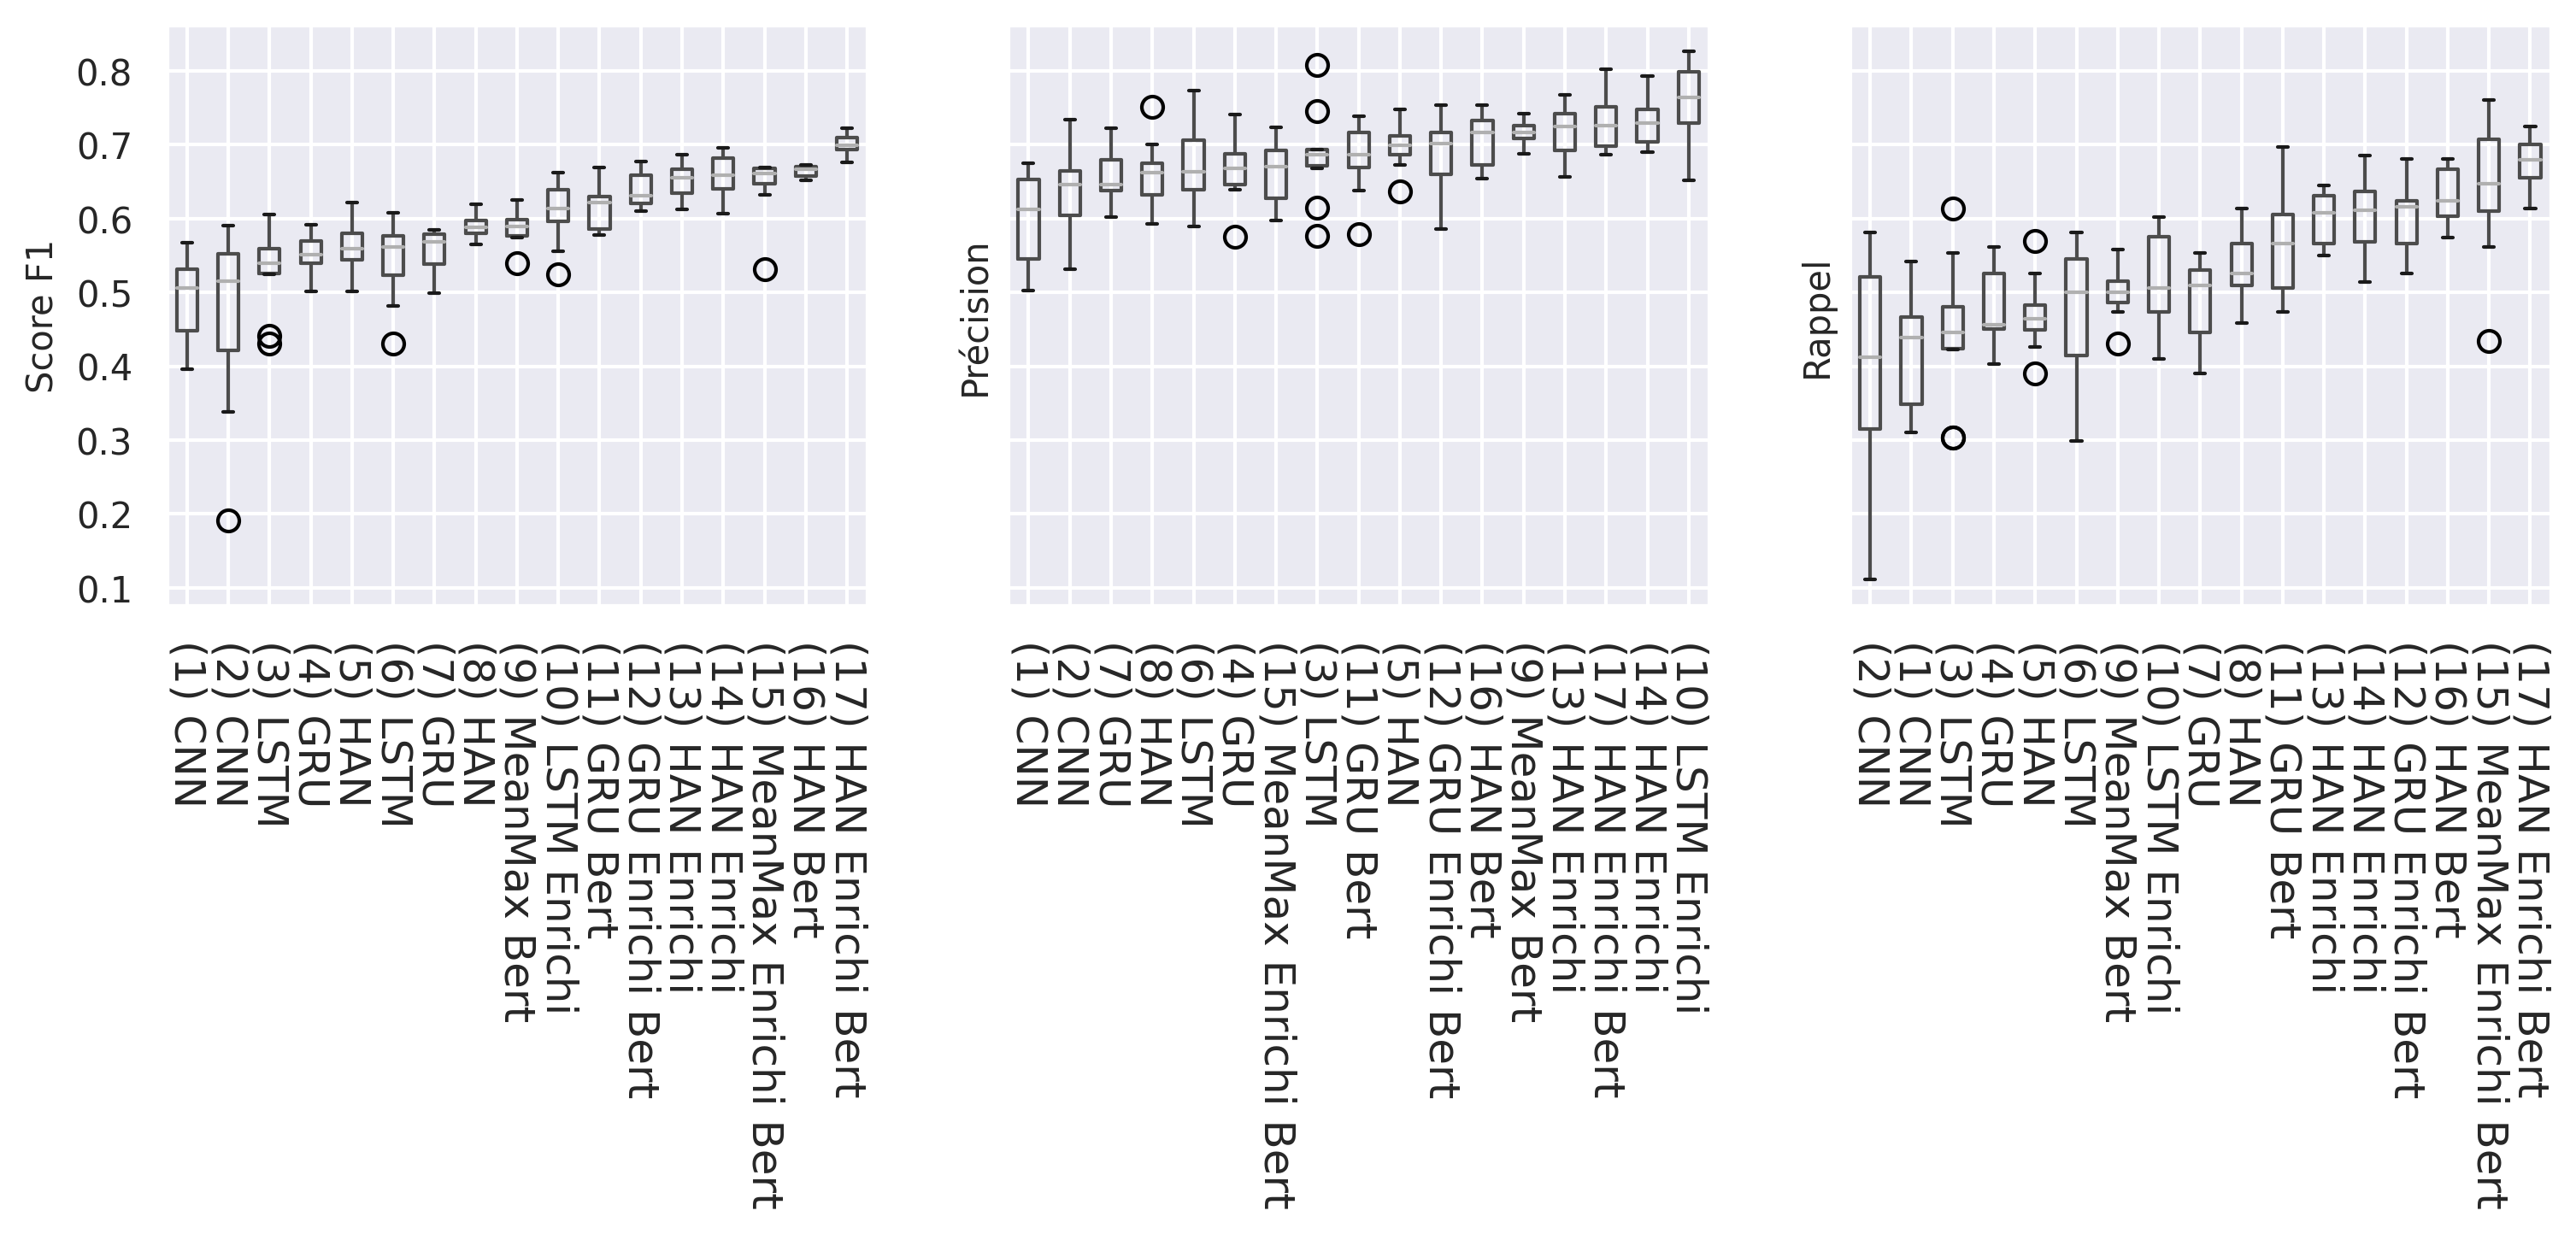
\includegraphics[width=\linewidth]{figures/chap4/partial-dispersionscores.png}
    \captionof{figure}{Dispersion des score sur le corpus partiel des meilleurs modèles, des modèles BERT et de modèles simples (CNN, GRU, HAN, LSTM sans enrichissements) sur 10 entraînements . Les détails sur les architectures sont donnés en table \ref{tab:chap4:partial-results}.}
    \label{fig:chap4:partial-results-dispersion}
    
\end{minipage}

% \subsubsection{Entraîner à partir de termes explicites uniquement}
%mentula, cunnus, pedico, futuo, culus ?

\subsubsection{Entraîner à partir de métaphores uniquement}

Le set de données Métaphores est un échantillonnage basé sur la présence du tag \texttt{\#metaphor} dans l'échantillon. Cet échantillonnage produit 459 échantillons positifs, répartis entre un corpus train (413) et un corpus dev (46). Le corpus de test est constitué de tous les textes n'incluant pas ce tag, y compris ceux marqués par \texttt{\#euphemism} ou \texttt{\#metonymy}, résultant en un corpus de test bien plus important de 2057 échantillons positifs (plus grand que le corpus d'entraînement du corpus principal). Si ce corpus a peu de probabilité d'être équivalent à un corpus compilé à la main en prévision de l'élargissement d'un modèle, il nous renseigne sur ce que peut comprendre le modèle sur le contexte implicite des isotopies sexuelles.

Les métadonnées permettent encore aux modèles de produire des résultats supérieurs aux autres (\textit{cf.} table \ref{tab:chap4:metaphor-results}). Mais ce sont les modèles BERT, y compris le modèle utilisant \textit{MeanMax} avec une couche linéaire enrichie qui bat les scores des autres modèles, le score de rappel étant le facteur le plus important de discrimination entre les modèles: environ 7 points d'écart entre le meilleur et le pire modèle en précision, tandis que presque 20 points séparent les modèles en rappel (\textit{voir} figure \ref{fig:chap4:metaphor-results-dispersion}). La prépondérance de \textit{MeanMax}, utilisant une moyenne des vecteurs de sous-tokens concaténée à la valeur maximale de ces sous-tokens, est exceptionnelle pour l'ensemble des expériences: 6 points en rappel séparent d'ailleurs le modèle \textit{MeanMax} du second, utilisant GRU comme encodeur. Dans ce modèle \textit{MeanMax}, seule la couche linéaire enrichie est donc entraînée, le \textit{pooling} et la projection ne nécessitant pas de spécialisation. Près de trois échantillons sur cinq sont ignorés par le modèle en test, mais au vu de la taille du set d'entraînement et de la variation possible dans le corpus de test, ce score est tout à fait louable.

Au contraire du modèle enrichi et du modèle sur corpus partiel, les modèles non enrichis utilisant BERT n'obtiennent pas cette fois-ci les meilleurs scores, qu'ils utilisent des encodeurs récurrents ou des systèmes de pooling. Il semblerait donc que le surentraînement provoqué par les métadonnées ``fait attendre'' des isotopies sexuelles plus que la simple projection effectuée par le \textit{transformer}: si \textit{MeanMax} enrichi est premier, il est aussi bon antépénultième quand il n'est pas enrichi, à 20,05 points de rappel derrière son alter ego.

Le premier modèle non enrichi, et potentiellement moins surentraîné, obtient un rappel à 9 points du premier modèle, ratant ainsi deux éléments positifs sur trois du corpus test. Sa précision reste excellente, comme celle de l'ensemble des modèles: peu des éléments qu'il sélectionne comme positifs sont de faux positifs (un tout petit peu plus d'un sur vingt). Avec un score aussi fort, d'un point de vue purement statistique, on peut attendre du modèle une détection fine de quelques traits saillants des isotopies sexuelles, en étant au contraire incapable de reconnaître des contextes plus vagues, peut-être plus crus. 

\noindent\begin{minipage}{\linewidth}%
    \resizebox{\linewidth}{!}{%}
    \begin{tabular}{r|lllll|rrr}
    \toprule
     Index & Morphologie & Encodeur & Enrichissement & Embeddings & Taille encodée &  Précision &  Rappel &  Score F1 \\
    \midrule
        19 &             &  MeanMax &         Linear &       BERT &            256 &      90.20 &   \textbf{42.05} &     \textbf{57.36} \\
        18 &             &      GRU &         Linear &       BERT &            256 &      92.17 &   36.49 &     52.28 \\
        17 &             &     LSTM &           LSTM &   FastText &            256 &      96.56 &   35.08 &     51.34 \\
        16 &             &      HAN &         Linear &   Word2Vec &            128 &      96.17 &   33.79 &     49.98 \\
        15 &             &     LSTM &           LSTM &   FastText &            128 &      \textbf{97.32} &   33.23 &     49.56 \\
        14 &  Agglomérée &      GRU &                &   Word2Vec &            256 &      94.87 &   \textbf{33.11} &     \textbf{49.05} \\
        13 &  Agglomérée &     LSTM &                &   Word2Vec &            256 &      95.36 &   32.77 &     48.71 \\
        12 &  Agglomérée &     LSTM &           LSTM &   Word2Vec &            128 &      95.01 &   30.31 &     45.91 \\
        11 &             &      HAN &         Linear &       BERT &            256 &      94.27 &   30.09 &     45.61 \\
        10 &  Agglomérée &      HAN &                &   Word2Vec &            256 &      95.98 &   29.39 &     45.02 \\
         9 &  Agglomérée &      GRU &                &   Word2Vec &            128 &      96.33 &   28.76 &     44.28 \\
         8 &  Agglomérée &     LSTM &           LSTM &   Word2Vec &            256 &      96.17 &   28.42 &     43.78 \\
         7 &  Agglomérée &     LSTM &                &   Word2Vec &            128 &      95.86 &   27.49 &     42.67 \\
         6 &             &      GRU &                &       BERT &            256 &      92.52 &   26.84 &     41.59 \\
         5 &  Agglomérée &      HAN &                &   Word2Vec &            128 &      95.34 &   26.54 &     41.45 \\
         4 &  Agglomérée &      CNN &                &   Word2Vec &            256 &      \textbf{96.75} &   23.07 &     37.31 \\
         3 &             &  MeanMax &                &       BERT &            256 &      91.73 &   22.00 &     35.52 \\
         2 &             &      HAN &                &       BERT &            256 &      92.71 &   21.93 &     35.46 \\
         1 &  Agglomérée &      CNN &                &   Word2Vec &            128 &      96.12 &   21.22 &     34.65 \\
    \bottomrule
    \end{tabular}%
    }
    \captionof{table}{Score médian sur le corpus Métaphores des meilleurs modèles, des modèles BERT et de modèles simples (CNN, GRU, HAN, LSTM sans enrichissements) sur 10 entraînements. En gras, les meilleurs scores des modèles avec enrichissement et sans enrichissement.}
    \label{tab:chap4:metaphor-results}
    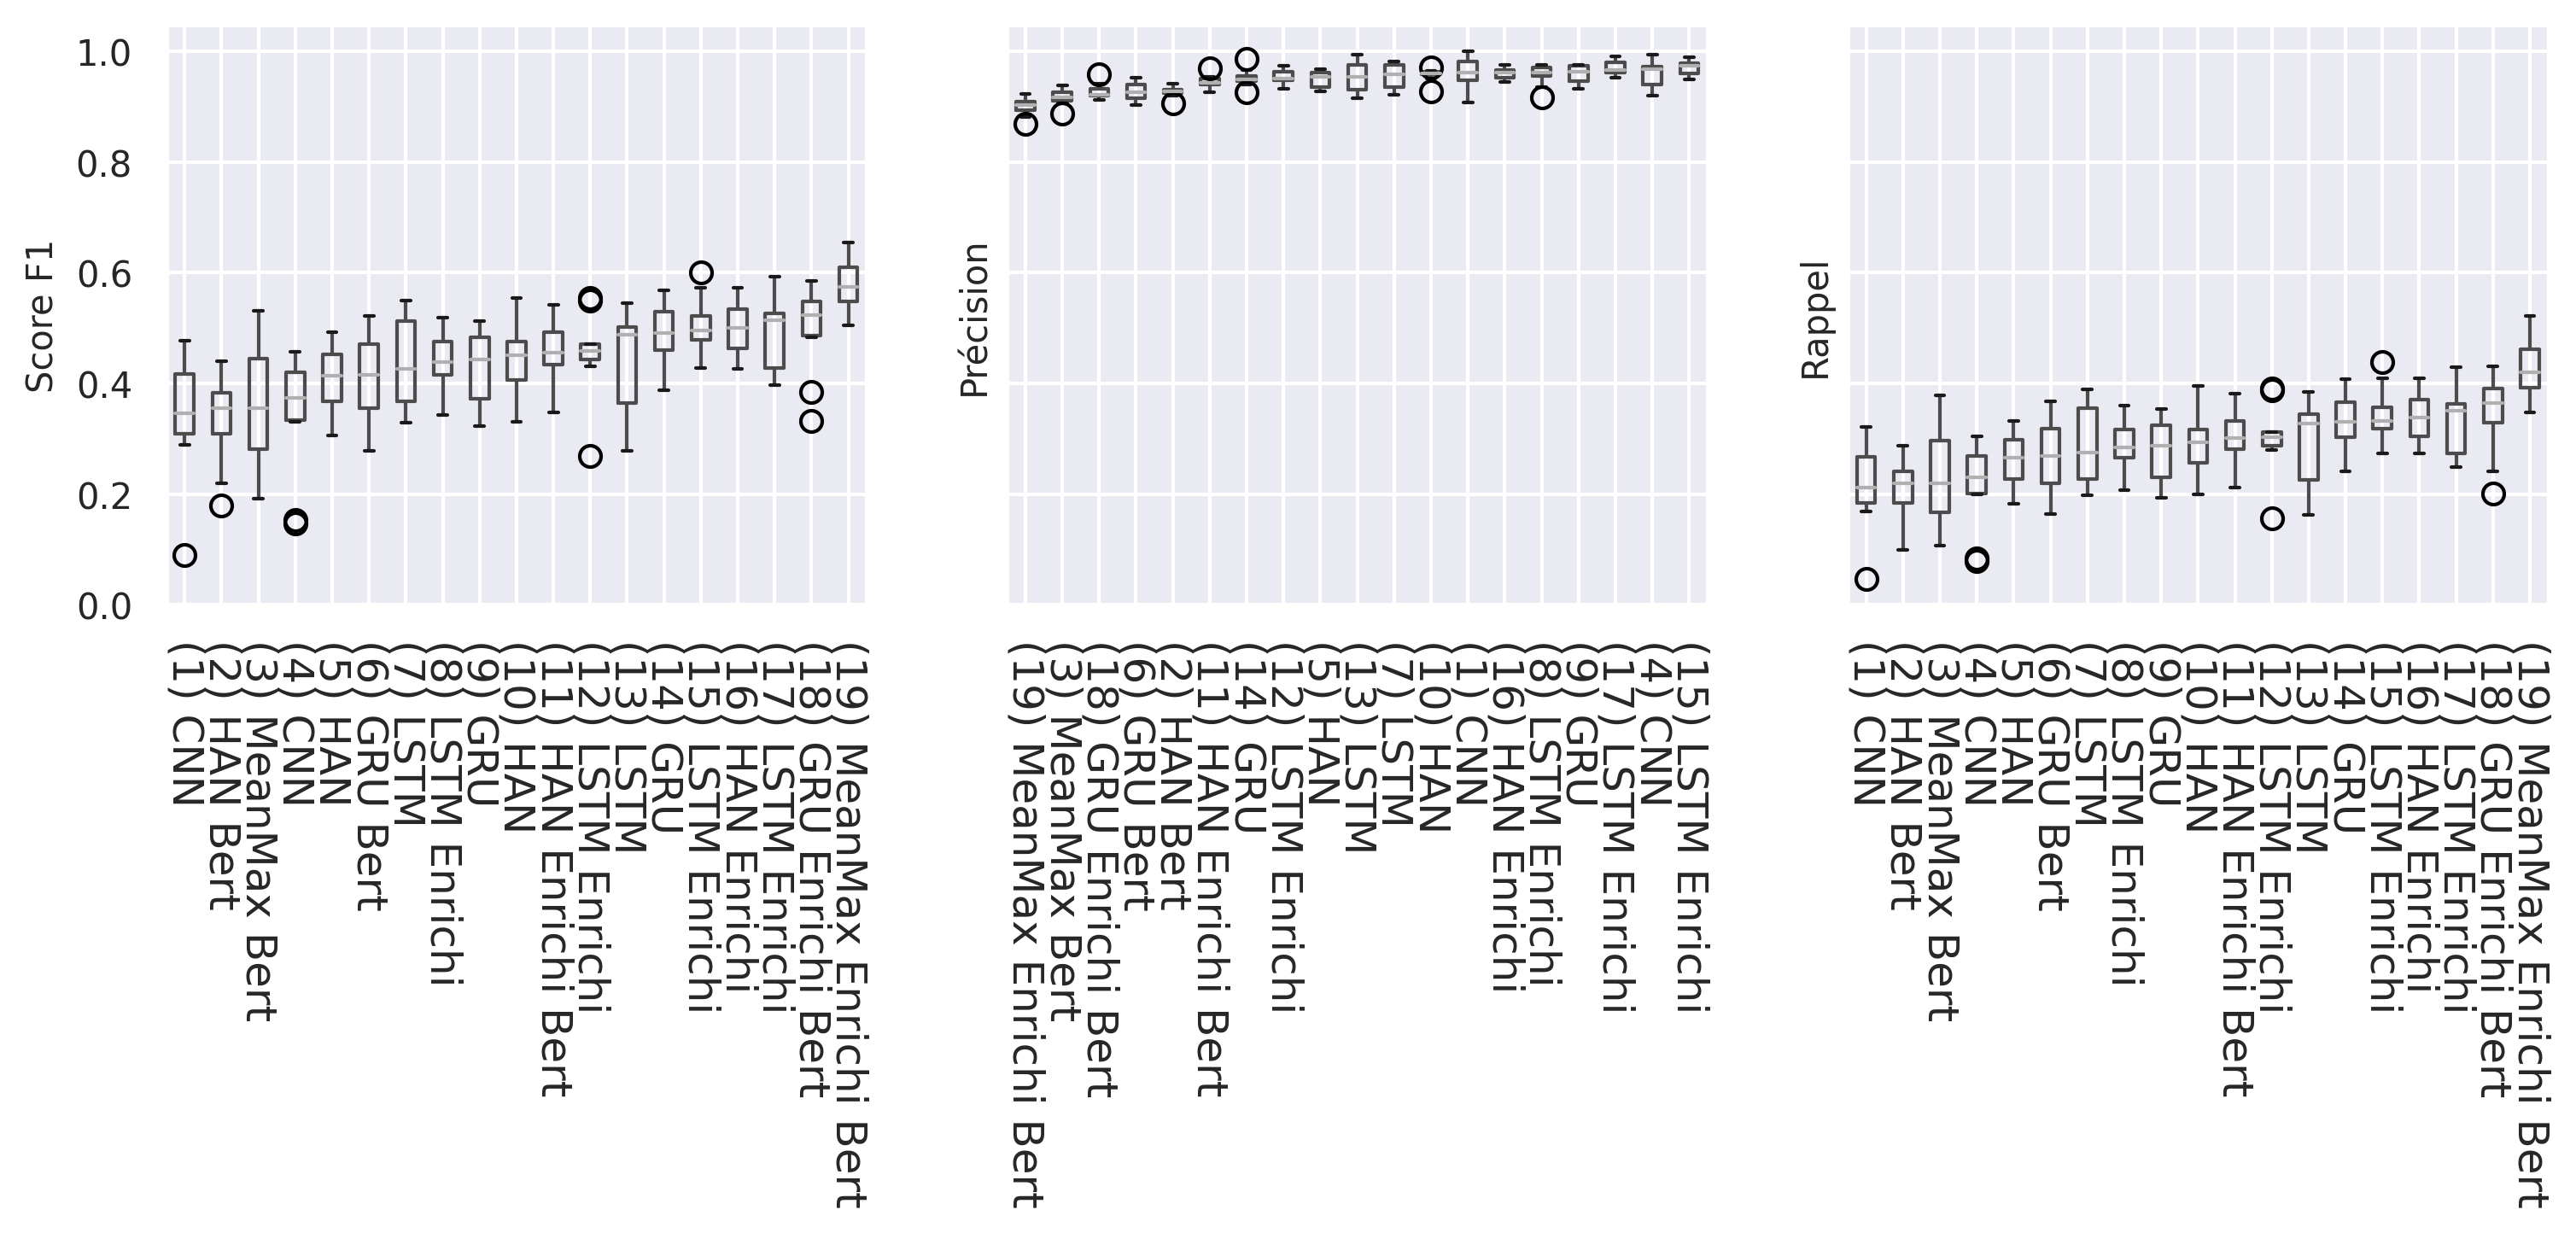
\includegraphics[width=\linewidth]{figures/chap4/metaphors-dispersionscores.png}
    \captionof{figure}{Dispersion des score sur le corpus Métaphores des meilleurs modèles, des modèles BERT et de modèles simples (CNN, GRU, HAN, LSTM sans enrichissements) sur 10 entraînements . Les détails sur les architectures sont donnés en table \ref{tab:chap4:metaphor-results}.}
    \label{fig:chap4:metaphor-results-dispersion}
\end{minipage}

% \subsubsection{Entraîner à partir de termes explicites uniquement}
%mentula, cunnus, pedico, futuo, culus ?

\subsubsection{La reconnaissance de métaphores}

Le set de données ``Non-Métaphores'' est issu d'un échantillonnage inversé de celui appliqué à Métaphores: les 459 éléments marqués par \texttt{\#metaphor} sont relégués en test, tandis que l'ensemble des autres éléments sont répartis entre train et dev. Le modèle contient ainsi 1439 documents positifs pour l'entraînement et 618 pour l'aiguillage de ce dernier. Il s'agit du second corpus le plus grand pour l'entraînement, derrière le corpus Général, et du plus grand corpus de dev, permettant potentiellement de mieux guider l'entraînement loin de la surspécialisation. Ce corpus ressemble plus, en dehors de sa quantité, à un corpus compilable manuellement: il reprend des termes ``intrinsèquement'' liés à l'isotopie sexuelle et dont l'interprétation laisse peu de doute (\textit{futuo}, \textit{mentula}, \textit{cunnus}, etc.); il prend en compte les cas de métonymies (\textit{mentulas cacare}\footnote{Littéralement ``Chier des bites'', pour parler de \textit{pedicatio}}, \textit{laxo}\footnote{Élargir, rendre plus lâche.}, \textit{scortum duco}, \textit{eo}\footnote{\textit{Aller} quelque part en vue de coucher.}) et d'euphémismes (\textit{res}, \textit{partes}), plus ``faciles'' à interpréter pour le compilateur humain. La capacité ou non d'un modèle à reconnaître des métaphores à partir de ce corpus nous informe donc sur la possibilité d'étendre le modèle à des usages plus complexes, à des développements plus figurés de l'isotopie sexuelle, telle que l'usage de \textit{columna} (la colonne) à la place du sexe.


Les modèles enrichis se partagent le top 10 des architectures avec les modèles classiques, le top 6 en score F1 étant composé uniquement des premiers et d'un modèle ``classique'' (\textit{cf.} table \ref{tab:chap4:literal-results}). L'écart cependant dans ce top 10 est bien faible en score F1, un peu plus de 4 points entre le premier et le dixième, sachant que près d'un point sépare déjà le premier et le second. Sur ce top 10, les modèles non enrichis obtiennent des rappels équivalents ou supérieurs aux modèles classiques, ratant environ deux exemples à métaphore sur cinq (l'écart est globalement faible, de l'ordre 5 points). C'est en précision, encore, que les modèles enrichis brillent: la surspécialisation sur les différents idiolectes ou sociolectes permet de sélectionner peu de faux positifs sur le corpus de test.

Confirmant une attitude remarquée sur les corpus les plus importants, les modèles BERT produisent les scores les plus faibles, malgré leur coût d'entraînement. Cependant, un \textit{MeanMax} enrichi sur la couche linéaire produit aussi le modèle avec le plus haut rappel, mais le plus faible taux de précision: s'il rate moins d'exemples positifs que ses concurrents, il a donc tendance à sélectionner trop de données faussement positives. Ce modèle est le seul avec un taux de rappel compétitif.

À partir d'un corpus ne contenant pas de métaphores, il est donc possible d'obtenir des modèles capables d'en détecter. Ainsi, le meilleur modèle sans enrichissement n'en rate que deux sur cinq dans notre corpus de test, et ne produit qu'un faux positif pour deux vrais positifs. Ces performances étant particulièrement hautes, et prometteuses dans le cadre de la production de corpus, l'hypothèse d'un biais de corpus doit être écarté. Or, le corpus de test ne partagent que 18,2\% de ses lemmes avec le corpus d'entraînement\footnote{$\frac{|Lemmes(Train)| \cap |Lemmes(Test)|}{|Lemmes(Test)|}$}, le plaçant à la troisième place de nos corpus d'expérimentation. Cette mesure est en effet de 30\% pour le corpus principal, 19\% pour le corpus partiel et 4,9\% pour le corpus Métaphores. D'autre part, la relative résistance des modèles sans enrichissements en métadonnées permet aussi d'écarter un score uniquement lié à un sur-apprentissage sur ces dernières. Ces hypothèses exclues, on peut donc estimer que le modèle est capable de reconnaître parmi ces répétitions de lemmes (quantifiables) ou de sèmes (beaucoup plus difficilement quantifiables) celles permettant de reconnaître une isotopie sexuelle construite via une métaphore.

\noindent\begin{minipage}{\linewidth}%
    \resizebox{\linewidth}{!}{%}
    \begin{tabular}{r|lllll|rrr}
    \toprule
     Index & Morphologie & Encodeur & Enrichissement & Embeddings & Taille encodée &  Précision &  Rappel &  Score F1 \\
    \midrule
        19 &  Agglomérée &      HAN &         Linear &   Word2Vec &            128 &      67.05 &   61.55 &     \textbf{64.03} \\
        18 &             &      HAN &         Linear &   Word2Vec &            256 &      65.78 &   59.59 &     62.86 \\
        17 &  Agglomérée &      GRU &                &   Word2Vec &            256 &      63.71 &   61.11 &     \textbf{62.16} \\
        16 &             &     LSTM &           LSTM &   FastText &            256 &      70.84 &   58.28 &     61.98 \\
        15 &             &     LSTM &           LSTM &   FastText &            128 &      69.12 &   56.32 &     60.63 \\
        14 &             &     LSTM &           LSTM &   Word2Vec &            128 &      \textbf{71.31} &   53.49 &     60.63 \\
        13 &  Agglomérée &      GRU &                &   Word2Vec &            128 &      64.98 &   57.84 &     60.50 \\
        12 &  Agglomérée &     LSTM &                &   Word2Vec &            128 &      61.71 &   59.59 &     60.48 \\
        11 &  Agglomérée &      HAN &                &   Word2Vec &            256 &      61.89 &   58.17 &     59.78 \\
        10 &  Agglomérée &     LSTM &                &   Word2Vec &            256 &      57.72 &   \textbf{61.33} &     59.38 \\
         9 &  Agglomérée &      HAN &                &   Word2Vec &            128 &      67.23 &   53.81 &     58.63 \\
         8 &             &      HAN &         Linear &       BERT &            256 &      67.19 &   52.40 &     58.20 \\
         7 &             &  MeanMax &         Linear &       BERT &            256 &      49.72 &   \textbf{68.63} &     57.32 \\
         6 &             &      GRU &         Linear &       BERT &            256 &      65.19 &   52.40 &     57.19 \\
         5 &             &      GRU &                &       BERT &            256 &      61.19 &   51.63 &     55.68 \\
         4 &             &      HAN &                &       BERT &            256 &      58.56 &   52.94 &     55.19 \\
         3 &  Agglomérée &      CNN &                &   Word2Vec &            256 &      \textbf{67.52} &   47.06 &     55.08 \\
         2 &             &  MeanMax &                &       BERT &            256 &      53.23 &   53.38 &     52.13 \\
         1 &  Agglomérée &      CNN &                &   Word2Vec &            128 &      63.36 &   38.89 &     48.36 \\
    \bottomrule
    \end{tabular}%
    }
    \captionof{table}{Score médian sur le corpus Non-Métaphores des meilleurs modèles, des modèles BERT et de modèles simples (CNN, GRU, HAN, LSTM sans enrichissements) sur 10 entraînements. En gras, les meilleurs scores des modèles avec enrichissement et sans enrichissement.}
    \label{tab:chap4:literal-results}
    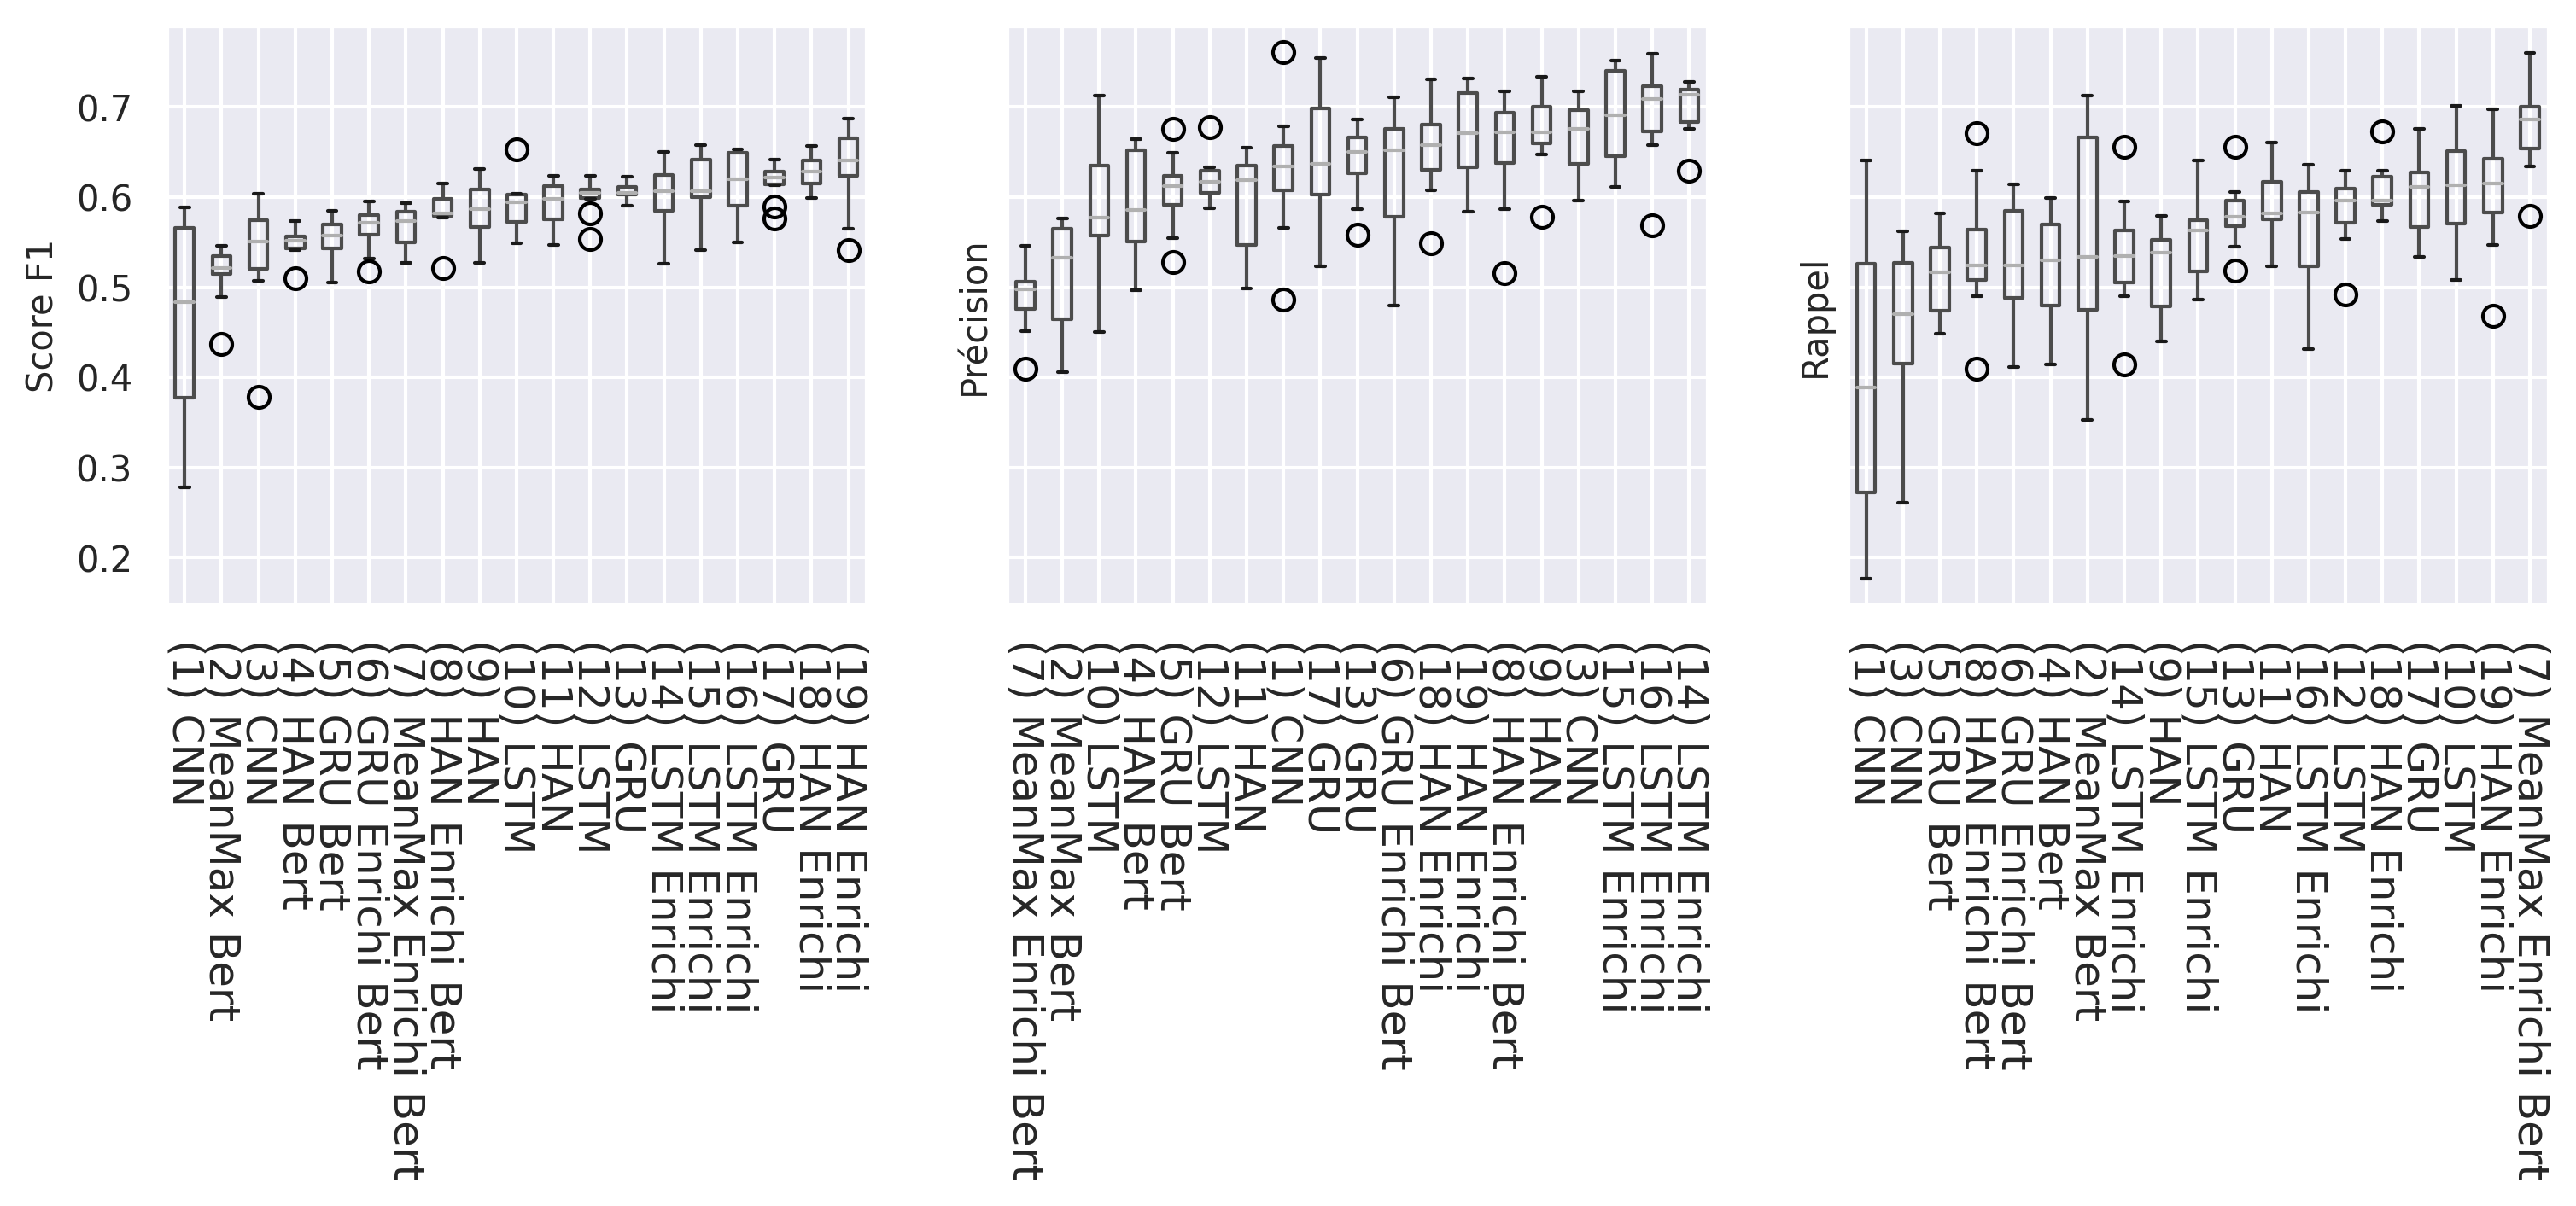
\includegraphics[width=\linewidth]{figures/chap4/literal-dispersionscores.png}
    \captionof{figure}{Dispersion des score sur le corpus Non-Métaphores des meilleurs modèles, des modèles BERT et de modèles simples (CNN, GRU, HAN, LSTM sans enrichissements) sur 10 entraînements . Les détails sur les architectures sont donnés en table \ref{tab:chap4:literal-results}.}
    \label{fig:chap4:literal-results-dispersion}
\end{minipage}

\section{Analyse des résultats}

\subsection{Mécanismes d’attention: variations en fonction des modèles}

%\paragraph{Une approche statistique de l'attention}

Pour rappel, le réseau HAN (\textit{Hierarchical Attention Networks}) que nous utilisons\footnote{\textit{cf.} \ref{part:chap4:architectures:variations-architectures:encodage}.} repose sur un système de pondération au moment de la classification nommée \textit{Attention}. Cette attention répartit 100\% de sa valeur sur l'échantillon (pour nous, une phrase), chaque mot prenant alors une part plus ou moins grande de cette dernière. Cette pondération est apprise par le modèle pendant sa phase d'entraînement et peut permettre aussi au lecteur humain de comprendre les facteurs ayant conduit à l'une ou l'autre des classifications. Dans une phrase où chacun des mots porte une importance quasi égale pour l'isotopie de la sexualité, une attention répartie également semble logique, comme dans la phrase ``\textit{lambebat medios improba lingua viros.}'' (\textit{cf.} figure \ref{fig:chap4:attention:repartie}). Au contraire, pour une phrase où seuls un ou deux mots portent toute la ``charge'' isotopique, comme ``\textit{Corrupit frater uxorem meam quam tyrannus violaverat''} (\textit{cf.} figure \ref{fig:chap4:attention:mono}), l'attention sera très inégalement répartie.

\begin{figure}
     \centering
     \begin{subfigure}[t]{0.45\textwidth}
         \centering
         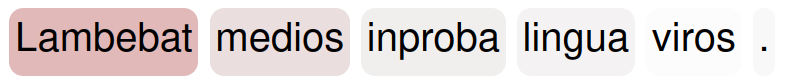
\includegraphics[width=\textwidth]{figures/chap4/attention.png}
         \caption{Martial, \textit{Épigrammes}, II.61.2. ``Sa langue perverse léchait le milieu des hommes.''}
         \label{fig:chap4:attention:repartie}
     \end{subfigure}
     \hfill
     \begin{subfigure}[t]{0.45\textwidth}
         \centering
         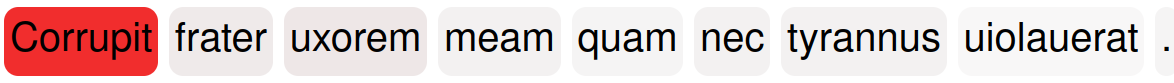
\includegraphics[width=\textwidth]{figures/chap4/attention2.png}
         \caption{Sénèque l'Ancien, \textit{Controverses}, I.7.4. ``Mon frère corrompit ma femme que même le tyran n'avait pas violée.''}
         \label{fig:chap4:attention:mono}
     \end{subfigure}
    \caption{Différentes répartitions de l'attention en fonction de l'interprétation du modèle. Plus le mot est sur fond foncé, plus il porte d'attention.}
    \label{fig:chap4:attention}
\end{figure}

En utilisant l'attention et les classifications produites par les architectures Morphologie+Word2Vec+HAN sans enrichissement sur le corpus test (scores médians sur la catégorie positive: meilleur pour le rappel hors architectures enrichies à 71,51\%, précision entre 82 et 84,5\% et score F1 à 76,50\%, \textit{cf.} table \ref{tab:chap4:general-results}), nous nous intéressons au rapport entre l'analyse de J. N. Adams et l'attention utilisée par le réseau. On récupère alors les informations suivantes:
\begin{itemize}
    \item Le rang en importance d'attention, 1 étant le mot portant l'attention la plus importante.
    \item La classification, positive ou non, ainsi que sa justesse (faux positif ou faux négatif).
\end{itemize}

\begin{figure}
    \centering
    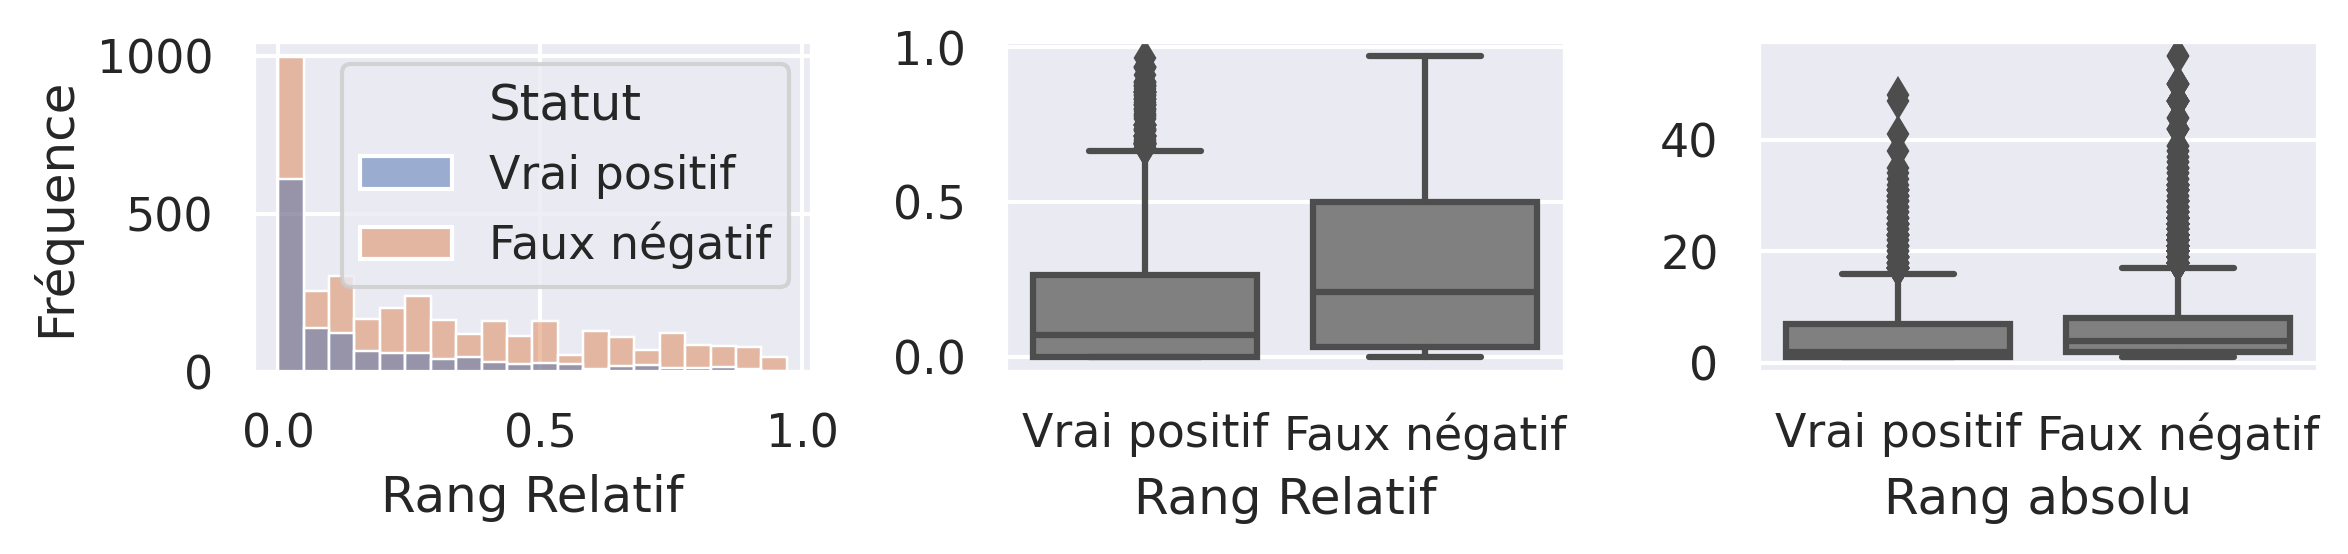
\includegraphics[width=\linewidth]{figures/chap4/ranksStatus.png}
    \caption{Rang relatif de l'attention dans les échantillons des termes relevés comme ``sexuels'' par J. N. Adams dans ces échantillons. Le rang relatif est calculé comme $\frac{Rang(Token)}{Nombre(Tokens)}$, ainsi, 0,0 ou 0,1 seraient dans les 10\% des mots les plus importants.}
    \label{fig:chap4:ranks-attention}
\end{figure}

Dans un premier temps, on s'intéresse à la capacité de l'attention à reconnaître dans chacun des documents échantillons l'importance du mot retenu par J. N. Adams dans son lexique. Pour faire cela, on analyse la fréquence des rangs de ces derniers. Si l'information est importante et intéressante, un terme n'obtenant pas le rang 1 n'est pas nécessairement ignoré, et l'on peut comprendre d'autres choix lorsque l'isotopie est portée par de multiples termes à forte charge sexuelle. Ainsi, dans la phrase ``\textit{cum cunno mihi mentula est uocanda. }'' (``Il faut appeler ça une bitte et ça une chatte.''), les mots \textit{mentula} (bitte) et \textit{cunnus} (chatte) portent tous les deux une importante forte. D'après l'analyse des termes et de leur rang en figure \ref{fig:chap4:ranks-attention}, on peut conclure que le modèle intègre largement les bons mots porteurs, avec quelques rares situations où il passe vraisemblablement à côté. Le rang médian des mots de J. N. Adams est en effet 2 (donc deuxième mot portant le plus d'attention) avec un rang relatif aux environs de 6\% des mots les plus importants de la phrase.

\begin{table}[]
    \centering
    \begin{tabular}{l|rrrr}
    \toprule
    Statut &  Faux négatif & Faux positif &  Vrai négatif & Vrai positif \\
    Lemme &               &              &               &              \\
    \midrule
    !     &         33.33 &         0.13 &         26.97 &              \\
    .     &          5.72 &         0.02 &         35.63 &         1.50 \\
    ;     &          3.38 &              &         22.28 &              \\
    ?     &          8.18 &              &         48.25 &         0.45 \\
    ,     &          0.01 &         0.00 &          0.11 &         0.06 \\
    \bottomrule
    \end{tabular}
    \caption{Pourcentage des signes de ponctuation qui se retrouvent en rang 1 de l'attention, sur 20 entraînements différents. Les points d'exclamation se retrouvant en premier rang de l'attention représentent 26,97\% des points d'exclamation des échantillons négatifs, qui sont classés en négatifs.}
    \label{tab:chap4:ponctuation-attention}
\end{table}

La distribution est différente chez les faux négatifs -- les éléments positifs mal reconnus par le modèle -- où la médiane du rang en attention du mot central d'Adams est de 4, et son premier quartile à 2 (contre 1 du côté des vrais positifs). En regardant les termes arrivés en rang 1 de l'attention des vrais négatifs et des faux négatifs, les signes de ponctuation sont parmi les formes les plus importantes retrouvées: à défaut de comprendre la phrase, le mécanisme d'apprentissage choisit des formes ``vides''. Cette réalité s'étend au-delà de la ponctuation, le top 10 des formes en rang 1 de l'attention chez les vrais négatifs comprenant ainsi \textit{et, sum, in, qui} et \textit{suus}. 

L'attention peut pour autant être ignorée en partie par le modèle au moment de la classification. Des termes importants tels que \textit{corrumpo} dans nos données positives se retrouvent 162 fois en rang 1 pour les vrais négatifs, et 120 fois pour les vais positifs. Le modèle arrive donc régulièrement à comprendre la polysémie de certains termes après avoir appliqué le phénomène d'attention\footnote{On le retrouve 36 fois en faux positif, 27 fois en faux négatif.}. Les termes \textit{voluptas, amor, uxor} sont ainsi parmi les 42 termes présents en rang 1 plus de 100 fois chez les vrais négatifs. Mais cette polysémie n'est pas toujours bien capturée comme le montre la présence dans les faux négatifs des termes \textit{libido, corrumpo} ou \textit{genitalis} (45 et 27) dans les cinq lemmes les plus fréquents en rang 1 d'attention\footnote{Les deux autres étant des signes de ponctuation: le point est présent 183 fois, le point d'interrogation 36.}.

\subsection{Erreurs et usage de l'attention}

Cette attention peut aussi être utile dans le cas d'une étude des faux positifs, échantillons sensés être négatifs dans notre set de données généré semi automatiquement, et des faux négatifs, échantillons classés par J. N. Adams comme positifs, mais non reconnus par le modèle. Nous proposons, en plus ainsi d'une approche statistique, un commentaire de quelques échantillons afin de mieux comprendre l'usage de ce mécanisme et sa possible responsabilité dans les erreurs. Dans les prochains exemples, le mot en gras et le nombre qui le suit sont le mot retenant le plus l'attention du modèle (rang 1) et le nombre de fois où il s'est retrouvé à ce rang sur 20 modèles répartis entre deux architectures de dix modèles chacune variant uniquement au niveau de l'encodage à 128 ou 256.

\subsubsection{Attention et faux positifs}

\begin{quote}[31]{\textit{Priapées}}
    \enquote{\textit{Donec proterua nil mei manu carpes ,{\\}  licebit ipsa sis \textbf{pudicior} Vesta . }} \\
    \enquote{Tant que tu ne cueilles rien chez moi d’une main effrontée, {\\} Tu pourras être plus pudique que Vesta elle-même.}
\end{quote}

Ici, \textit{pudicior} reçoit l'attention du modèle et donne une phrase positive 25\% du temps sur 20 modèles. Et le modèle a raison: on est face ici à une traditionnelle menace sexuelle de Priape, gardien des jardins et vergers (visible dans d'autres priapées telles que les 13, 17 -- avec la même idée ``d'élargissement de l'anus''--, 22, etc.). Par implication, on comprend qu'il y a une punition en cas de vol. La force de l'adynaton formé par le comparatif et le comparé -- on ne peut pas être plus pudique que Vesta -- ne laissent cependant que peu de doutes sur ce qui sera réservé au porteur d'une main voleuse. L'alternative sous-entendue en opposition à \textit{pudicior} est celle d'une \textit{pedicatio}, confirmée par les vers suivants. L'usage des adjectifs moraux tels que \textit{pudicus}, en hyperbole ou non, sont un des angles morts du corpus de J. N. Adams.

\starbreak

\begin{quote}[\textit{Epitome anonyma (quae gynaecia uocatur)}, recension Li]{Vindicianus Afer}
    \textit{et est a foris neruosa \textbf{uulua} , cuius collum directum est positum , cuius ceruix erigitur usque ad locum , in quo res Veneris perficiuntur et sperma miscetur et fit conceptio natura uolente ex uiri et mulieris sanguine .} \\
    \enquote{Et l'uterus est musclé par l'extérieur, son cou est aligné avec ce lieu, son cou s'étend jusqu'au lieu, dans lequel les choses de Venus sont accomplies et où le sperme se mélange et où la conception, si la nature le veut, se fait du sang de l'homme et de la femme.}
\end{quote}

\begin{quote}[\textit{Epitome anonyma (quae gynaecia uocatur)}, recension Li]{Vindicianus Afer}
    \enquote{\textit{Ego cum muliere menstruata concubui et non concepit, nam purgacionis plurimo sanguine minor pars seminis \textbf{corrupta} (50.00) est.}} \\
    \enquote{Moi, je partageai mon lit avec une femme ayant ses règles et (pourtant ?) je ne me reproduisis pas, car une petite partie de ma semence fut corrompue par une grande quantité du sang de ce curage.}
\end{quote}

\begin{quote}[\textit{Formulae spiritalis intelligentiae}, 6]{Eucher de Lyon}
    \enquote{\textit{{[}Umbilicus appetitus concupiscentiae. in Iob: et uirtus eius super umbilicum uentris, id est.{]}\footnote{Nous ajoutons le contexte pour la compréhension de la phrase, car l'échantillon pourrait être mal ponctué dans la source d'origine.} Quod feminae \textbf{genitalia} (52.50) per hoc significet sicut in lumbis\footnote{\textsc{Lumbus} comme parties sexuelles masculines ou féminines, \textit{cf.} \textcite[p.~48]{adams}} uirorum.}} \\
    \enquote{Le nombril a est le lieux des penchants pour la concupiscence. Chez Job, ses qualités sont au dessus du centre du ventre, c'est-à-dire que les organes génitaux de le femme expriment à travers-lui la même chose que dans les organes génitaux des hommes.}
\end{quote}

\begin{quote}[\textit{De salutaribus praeceptis}, 28]{Caelius Aurelianus}
    \enquote{\textit{{[}Intellegimus virum{]} ex asperitate faucium, obtunsione vocis et rauco sonitu, inflatione etiam papillarum et \textbf{genitalium} (50.00) , et cum repente maceratum corpus in longitudinem viderimus porrectum.}}
    \enquote{{[}Nous reconnaissons l'homme{]} à travers l'âpreté de la gorge, le fracas de la voix, à son bruit rauque mais aussi au gonflement des seins et de ses organes génitaux, et lorsque nous avons vu son corps soudainement épuisé étendu en longueur.}
\end{quote}

Il s'agit encore de faux positifs ``vrais positifs'', donc des données d'entraînement mal classées et non répertoriées par J. N. Adams et le LLT, de données présentant des problèmes de lemmatisation qui ont empêché le recensement, ou enfin de données qui étaient absentes du corpus au moment de la compilation du catalogue d'exemples.

Ces quatre extraits de trois auteurs différents sont tous tardifs et proposent tous une analyse des corps, qu'il s'agisse de discours médicalisant chez Caelius Aurelianus et Vindicianus Afer, ou d'interprétation du rôle de chaque partie du corps dans une exégèse chez Eucher. Les mots qui y retiennent l'attention sont majoritairement connus du corpus d'Adams du lexique médical de la sexualité (\textit{vulva, genitalia, genitalium, seminis}). Pour \textit{corruptus}, précédé de \textit{seminis} (fr. semence), on se trouve face à deux tropes classiques de l'expression de la sexualité en latin: d'une part, la corruption (notamment des moeurs en latin tardif; d'autre part, d'un sperme ou d'une relation sexuelle corrompue par les règles. Particularité du premier extrait de Vindicianus, d'après le commentaire de Louise Cilliers sur une recension différente\footcite[p.236]{cilliers_vindicianuss_2005}, l'alternance \textit{collum}/\textit{ceruix} servirait à éviter une répétition et désignerait \textit{in extenso} le vagin (\textit{cuius collum}: le cou de la matrice), là où \textit{vulva} désignerait l'utérus et non ce que l'on appelle aujourd'hui la vulve.

\starbreak

\begin{quote}[Jonas, 2, 2]{\textit{Vulgate}}
    \enquote{\textit{et oravit Iona ad Dominum Deum suum de \textbf{utero} (27.50) piscis}} \\
    \enquote{Et Jonas émit des prières à son Seigneur Dieu depuis le ventre du poisson.}
\end{quote}

\begin{quote}[\textit{Héroïdes}, 16, 43]{Ovide}
    \enquote{\textit{Matris adhuc \textbf{utero} partu remorante tenebar;}} \\
    \enquote{L'accouchement tardant, j'étais retenu jusqu'ici dans le ventre de ma mère.}
\end{quote} 

\starbreak

Ici encore, c'est \textit{uterus} qui récupère la majeure partie de l'attention. S'il arrive bien que des poissons soient mêlés à des descriptions d'actes sexuels (\textit{cf.} Suétone, \textit{Tibère}, 44), il ne s'agit pas dans l'extrait de la Vulgate d'un \textit{uterus} mais bien d'un ventre. Dans le même genre que les précédents faux vrais positifs, il est plus que probable que -- chez Ovide -- \textit{uterus} représente bien le ventre et non l'organe génital féminin: il n'y a pas de discours médicalisant, il n'y a pas de raison de s'attendre à un usage aussi précis du mot \textit{uterus}. La présence de \textit{partus} (fr. accouchement) et de \textit{matris} (fr. mère) a pu conduire le modèle à interpréter le terme \textit{uterus} plus médicalement qu'Ovide ne le souhaitait. Dans les deux cas, le modèle s'est définitivement fait tromper par la polysémie du mot \textit{uterus}, spécialisé chez les auteurs médicaux.

\begin{quote}[\textit{Amours}, 3, 28]{Ovide}
    \enquote{\textit{\textbf{Nox} (10.00) tibi, si belles, possit, Homere, dari.}} \\
    \enquote{Si tu avais fait la guerre, Homère, la nuit aurait pu t'être donnée.}
\end{quote}

Cette métaphore d'Ovide est ignorée par notre set d'entraînement et tombe encore dans le domaine de l'isotopie sexuelle. ``La nuit aurait pu t'être donnée'' porte clairement le sens sexuel à travers l'idée d'activités nocturnes. On peut être assez étonné et ravi de la capacité du modèle à retenir ce choix, dans la mesure où aucun terme personnalisant les acteurs sauf le vague \textit{tibi} n'est présent dans la phrase analysée, et qu'Homère n'est jamais présent dans notre set de données. \textsc{Nox} y est cependant présent 59 fois, dont un usage similaire avec le verbe \textsc{do} chez Ovide (\textit{Hic mihi lasciva gaudia nocte dedit}, ``Là elle me donna dans la nuit des joies lascives'', \textit{Remèdes à l'Amour}, 727; \textit{Est data nox ?}, ``La nuit t'est-elle donnée ?'', \textit{Remèdes à l'Amour}, 523) et des phrases similaires où la nuit est bien liée aux affaires du sexe (\textit{Date illi vestem puellarem, date noctem: rapietur.}, ``Donnez-lui des habits de jeunes filles, donnez-lui la nuit: il se fera violer'', Sénèque l'Ancien, Controverses, 5, 1). Adams note cet usage de $nox=stuprum$\footcite[p.178]{adams} mais omet son usage avec \textit{do}.

\starbreak

\begin{quote}[\textit{Mathesis}, 4, 14, 17]{Firmicus Maternus, Julius}
    \enquote{\textit{in uenerio \textbf{coitu} (60.00) facit libidinosos et uitiis quibusdam semper implicitos et qui adsiduis ob haec pulsantur infamiis.}} \\
    \enquote{[La lune] produits des libidineux dans leurs coïts vénériens, des hommes toujours entourés de certains vices, et, à cause de cela, des hommes qui sont frappés par des déshonneurs sans fins.}
\end{quote}

Texte particulier parmi les exemples vus jusqu'ici, \textit{Mathesis} est une oeuvre -- entre autres -- d'astrologie, et on a un extrait ici décrivant l'effet qu'a la pleine lune, se dirigeant de Mercure à Vénus, sur les hommes naissant pendant ce trajet. Tout le vocabulaire de la condamnation morale de l'excès de sexualité est présent: \textit{libidinosos, coitu venerio, uitiis}. %On pourrait même poser la question d'un choix volontaire de \textsc{pulso}, terme utilisé aussi pour les pulsions sexuelles (pulsations du sexe par exemple \textbf{A VERIFIER}). 
Le texte n'est donc pas en soi difficile à classer, ni pour la machine, ni pour le lecteur humain.

\starbreak

\begin{quote}[\textit{Mercator}, 13]{Plaute}
    \enquote{\textit{ibi amare occepi forma eximia mulierem.}} \\
    \enquote{Là, je commençais à aimer une femme à la beauté remarquable.}
\end{quote}

Faux positif qui est bien un négatif, la classification effectuée par le modèle peut sembler logique, tant le lexique présent est typique des isotopies sexuelles: \textsc{mulier} est présent 76 fois dans notre set de données, \textsc{amo} 20 fois, \textsc{forma} 19 fois. Autant de formes lexicales qui, mises bout à bout, pourraient avoir un sens particulier. Au contraire, si l'hypothèse de l'actualisation géotemporelle \textsc{ibi} poussant le modèle à classifier en isotopie sexuelle nous avait paru alléchante, l'absence d'une attention forte sur le thème et sa très très faible présence dans le corpus des échantillons poussent à en ignorer l'importance dans la classification. Hors contexte, il serait plus facile de comprendre une interprétation d'\textit{amo}=\textit{futuo} si \textit{forma eximia} (\enquote{à la beauté remarquable}) n'était pas présent.

\subsubsection{Attention et faux négatifs}

\begin{quote}[\textit{Caligula}, 41, 2]{Suétone}
    \enquote{\textit{misit circum fora et basilicas nomenculatores ad inuitandos ad \textbf{libidinem} (20) iuuenes senesque;}} \\
    \enquote{Il envoya des esclaves nomenclateurs à travers le forum et les lieux de promenades pour inviter jeunes et anciens à la débauche.}
\end{quote}

\begin{quote}[\textit{Horace, Satyres}, 1, 5, 100]{Porphyrion}
    \enquote{\textit{Vrbanissimum nomen Iudaeo inposuit ‘Apellan’ dicens , quasi quod pellem in parte \textbf{genitali} (19) Iudaei non habeant .}} \\
    \enquote{Il assigne un nom extrêmement spirituel au Juif en l'appelant ‘Apella’, sous prétexte que les juifs n'ont pas de peau sur les parties génitales. \footnote{Porphyrion fait ici un rapprochement entre une préfixation privative \textit{a-} et le mot ``pellis'' (peau) et le nom hébreux d'Apellas, pour justifier le jeu de mot d'Horace. \textcite{cordier2001romains}}}
\end{quote}

\begin{quote}[\textit{De Medicina}, 77]{Cassius Felix}
    \enquote{\textit{Sic enim \textbf{matrix} (14) poterit fetidis odoribus a superioribus ad inferiora fugari et loco proprio reuocari , cum melioribus et iocundis ad inferiores partes fuerit inuitata et prouocata.}} \\
    \enquote{Car ainsi, la matrice pourra être l'objet de fuite d'odeurs fétides des parties supérieures vers les parties inférieures et être ramenée à un lieu propre (être ramenée à sa qualité de lieu propre ?) lorsque les parties vers le bas auront été invitées et excitées par de meilleures et plus agréables choses (odeurs ?).}
\end{quote}

Ces trois premiers exemples, bien que légèrement différents, ne laissent pas beaucoup de doute sur le sens des mots sélectionnés. 

Du côté de Suétone, \textit{libido}, proche de \textit{iuvenes senesque} et en complément d'\textit{inuito}, est facile à interpréter, y compris hors contexte, pour le lecteur humain. Le contexte de l'extrait confirme le choix de J. N. Adams (mise en place de lupanar au palais). Le modèle retient bien l'attention 100\% du temps sur le terme relevé par J. N. Adams, mais décide de ne pas le classer positif, probablement à cause de sa polysémie, avec une décision d'un poids médian de 93,44\% en faveur de la catégorie négative sur les 20 entraînements. On peut faire l'hypothèse que la présence de \textit{forum} (bien qu'il soit 6 fois dans le corpus d'Adams et qu'il ne soit pas inconnu dans ce genre de contexte, il y est même plus présent que \textit{inuito}), de \textit{nomenclatures} et \textit{basilicas} puisse pousser le modèle vers une autre lecture de \textit{libido} par le modèle, face à ce vocabulaire du monde ``public'' voire administratif.

Pour l'extrait de Porphyrion, commentateur d'Horace, comme pour Cassius Felix, le résultat est plus difficile à comprendre. Dix-neuf fois sur vingt, le modèle a classé la première phrase comme négative  (taux médian de 95.5\%) et a retenu l'importance de \textit{genitali}, co-occurrent de \textit{parte} par ailleurs. Pour la seconde, il la trouve négative à chaque test avec 95,5\% de score médian, sélectionne quatorze fois \textit{matrix} (deux fois \textit{prouoco} et une fois chacun des tokens suivants: \textit{fetidus, et, ``.'', }), mais il estime que la phrase ne parle pas de sexualité.

Dans le premier exemple, la sexualité n'y est pas présente par acte: on a bien ici une description d'une partie de l'anatomie masculine avec une mention du rite de circoncision. Dans le \textit{De medicina}, on a aussi une discussion anatomique, mais il y a des éléments qui rappellent l'acte sexuel. Cependant, dans la compréhension d'Adams de la sexualité, c'est-à-dire ce que qui concerne les sexes dans leur rôle reproductif ou ludique, il y a bien ici une isotopie sexuelle. On voit avec ces exemples comment le modèle s'est peut-être ``trop'' éloigné de l'approche lexicométrique en refusant de compter des mots peu ou pas du tout polysémique.

Le problème n'est en tout cas pas du côté de l'attention, quel que soit l'extrait pris en compte ici. Les trois phrases ont leur mot le plus important entre 8 et 28 points au-dessus de la médiane des attentions. Le mécanisme est donc fonctionnel, d'autant que pour la distance la plus basse (Cassius Felix), il s'agit aussi de la phrase la plus longue (et mécaniquement d'une dilution de l'attention). Il s'agit donc d'un problème dans l'encodeur, une fois l'attention appliquée, ou de la couche de décision.

\starbreak

\begin{quote}[\textit{Casina}, 963]{Plaute}
    \enquote{\textit{nunc tu si vis \textbf{subigitare} (17) me, probast occasio.}} \\
    \enquote{Maintenant, si tu veux me caresser, c'est le bon moment.}
\end{quote}

\textit{Subigito} (\textit{Gaffiot}: caresser, solliciter; \textit{Adams}: \textit{make advances to, lay hands on}\footcite[p. 323]{adams_prostitute}) est un cas complexe, y compris dans son interprétation par J. N. Adams. Pour ce passage, on vient d'assister à une ruse ayant eu pour conséquence la rencontre sexuelle de deux hommes dans le noir, eux qui croyaient retrouver une jeune femme dans l'intimité d'une chambre. D'après J. N. Adams, Plaute utilise parfois le verbe ``dans un sens sexuel, mais léger''. Hors contexte ou en contexte, le doute reste permis sur le sens des caresses mentionnées, bien que les moeurs marseillaises -- \textit{a priori} liées à l'homosexualité masculine -- mentionnées au vers précédent, la mention de la chambre et la scène antérieure nous poussent à croire à des caresses sexuelles. La phrase est classée positivement deux fois, dix-huit fois négativement avec \textit{subigito} en rang 1 dix-sept fois (25 points d'attention en moyenne) et le point final une fois.

\starbreak

\begin{quote}[\textit{Épigrammes}, 11, 51]{Martial}
\textit{Tanta est quae Titio columna pendet , Quantam Lampsaciae colunt \textbf{puellae} (15) .}\\
\enquote{La colonne qui pend à Titius est si grande que les jeunes filles de Lampsaque la vénèrent.}
\end{quote}

Pour cette phrase, l'attention médiane est portée presque uniquement sur la consécutive (score médian d'attention entre parenthèses: \textit{Quantam (7,2) Lampsaciae (10,3) colunt (11,8) puellae (20,0) . (13,2)}) tandis que le mot central, \textit{columna}, bien qu'utilisé figurativement et très clair en termes de représentation, est assez largement ignoré par le mécanisme (médiane de 5 d'attention). La métaphore de la colonne n'est que peu présente dans notre set (Martial, 6, 49, 1; \textit{Priapées}, 10, 7) et celle des objets ``pointus'' en général aussi (38 occurrences, principalement des armes). Cette méconnaissance du domaine et le difficile rapprochement ont dû faire naître l'impossibilité pour le modèle de comprendre la portée de cette ``colonne''. On notera  tout de même que la question des jeunes filles ``intriguent'', si l'on peut dire ainsi, l'attention dans cette classification.

\starbreak

\begin{quote}[11, 51]{Pétrone}
    \enquote{\textit{Ego sic perire coepi\textbf{.} (15)}}\\
    \enquote{Et c'est ainsi que, moi, je commençai à mourir.}
\end{quote}

\begin{quote}[\textit{Satyricon}, 130]{Pétrone}
    \enquote{\textit{Paratus miles arma non habui\textbf{.} (13)}} \\
    \enquote{Prêt comme un soldat, des armes, je n'en avais pas.}
\end{quote}

\begin{quote}[\textit{Amours}, 3, 4, 4]{Ovide}
    \enquote{\textit{Quae, quia non liceat, non facit, illa facit \textbf{!} (14) }}\\
    \enquote{Celle qui ne fait pas, parce que c'est interdit, elle le fait !}
\end{quote}

\begin{quote}[\textit{Épigrammes}, 104, 9]{Ausone}
    \enquote{\textit{tergum, colla, umeros, luteae Symplegadis antrum\textbf{.} (13) }} \\
    \enquote{Son dos, son cou, ses épaules, son antre boueuse des Symplégades}
\end{quote}

Pour les quatre extraits, l'attention réagit de manière similaire: elle sélectionne la ponctuation finale de l'extrait comme portant l'ensemble de l'attention, comme elle le fait pour une majorité de faux négatifs (\textit{cf.} \ref{tab:chap4:ponctuation-attention}). Les quatre sont de faux négatifs présentant un manque d'indices sur l'isotopie sexuelle: c'est à chaque fois le contexte qui peut aider à s'assurer de cette classe. Les quatre exemples présentent un taux de classification médian fort (89\% et plus) avec une attention assez également répartie sur la phrase.

Chez Pétrone, les deux passages sont inégalement difficiles à comprendre. Le premier nécessite absolument le contexte et s'éloigne d'autres passages cités par Adams reprenant l'idée de la mort comme fin des ébats sexuels (par exemple, \enquote{Lorsque nous te vîmes, Gallus, mourir de l'étreinte d'une jeune fille}\footnote{\enquote{\textit{cum te complexa morientem, Galle, puella uidimus}}, Prop. 1, 10, 5. \textcite[p.159]{adams}}). Le second arbore tout un vocabulaire militaire, commun aux figures sexuelles, mais qui, sans autres indices dans l'extrait (présence d'une jeune fille par exemple), reste difficile à classer. Nous ne sommes pas dans le même cas de figure que la priapée à la \textit{Pudicior Vesta}: il n'y a pas d'exagération, de contexte ou tout simplement de temps permettant à l'isotopie de se déployer en aussi peu de mots qui partagent tous le même type de sèmes (exemple 2) ou sont entourés de termes presque vides (exemple 1).

Chez Ovide, le problème est le même que le premier extrait de Pétrone. Si \textit{facio} signifie ici \textit{futuo} ou \textit{pedico}\footcite[p.204]{adams}, en dehors de l'indice d'interdit, il n'y a rien qui ne pousse nécessairement vers le sexe, sans contexte. C'est le contexte des \textit{Amours} (au vers précédent, répétition de \textit{casta est} (elle est chaste), au vers suivant \textit{adultera}) qui nous aide à traduire. Mais sans ce contexte, le vers est difficilement classable, même pour le lecteur humain.

Pour le dernier extrait, deux problèmes se posent. D'une part, l'extrait est incomplet, très court, recopié tel qu'il fut cité par Adams, bien qu'il soit cité plusieurs fois\footcite[pp.114, 172 et 240]{adams}. Ici, ce sont les Symplégades -- deux falaises se faisant face et pouvant rappeler deux fesses dans l'esprit de l'auteur --, ``l'antre'' et le caractère boueux qui induisent une lecture sexuelle, mais cette métaphore \textit{ad-hoc}, reprise de chez Martial\footnote{\textit{sic {[tunicae]} constringuntur magni Symplegade culi} (Ainsi tes tuniques sont resserrées par les Symplégades jumelles de ton cul.), Martial, 11.99.5.}, est probablement l'une des plus difficiles à comprendre pour le modèle. Le contexte aide un peu dans la mesure où l'épigramme mentionne clairement au vers précédent un \textit{prurignis obscenae} (fr. démangeaison obscène) et avant encore des \textit{lascivos coetus meretricum} (fr. unions lascives de prostituées), mais les co-occurrents des Symplégades, \textit{antrum lutae}, restent plus compréhensibles que la métaphore topologique.

\starbreak

\begin{quote}[37, 9]{Catulle}
    \enquote{\textit{namque totius vobis frontem tabernae sopionibus scribam\textbf{.} (11)}} \\
    \enquote{Et de fait, je ferai des tags de queues (bites ?) sur le fronton de toute votre taverne.}
\end{quote}

Terme rare, unique dans le corpus, \textit{sopionibus} (queue, pénis ?) n'est pas retenu par le modèle. Étant seulement dans le corpus de test, il est impossible pour le modèle de comprendre le mot par le contexte (après tout, il est possible de dessiner bien des choses).

On voit ainsi que pour les faux négatifs, le problème vient, en dehors de quelques cas peu défendables, d'un problème de contexte ou de rareté. Le modèle, n'ayant pas assez d'indices, glisse sur les termes importants, et la traite comme elle traite beaucoup des négatifs, en n'en retenant que la ponctuation.

\subsection{Erreurs communes, phrases impossibles ?}

Pour conclure cette analyse de résultats, on s'intéresse aux impossibles ou quasi impossibles: sur quelles phrases les modèles ont-ils été incapable de se mettre d'accord avec la vérité de terrain. 

Pour analyser ces phénomènes, on récupère pour chaque modèle les résultats de classification de chacune des phrases, positives ou négatives. Par corpus, on obtient pour chacune des phrases un taux de non-reconnaissance (nombre de fois où la phrase a été mal reconnue divisée par le nombre de tests) et on s'intéresse alors aux phrases pour lesquelles ce taux est équivalent à 100\%. On tient cependant deux sets de phrases différents pour chacun des corpus: l'un composé des meilleurs modèles -- y compris enrichis -- et des modèles ``classiques'' sans enrichissement (120 entraînements et tests), l'autre composé uniquement des modèles ``classiques'' (80 entraînements et tests).

\begin{figure}[ht]
    \centering
    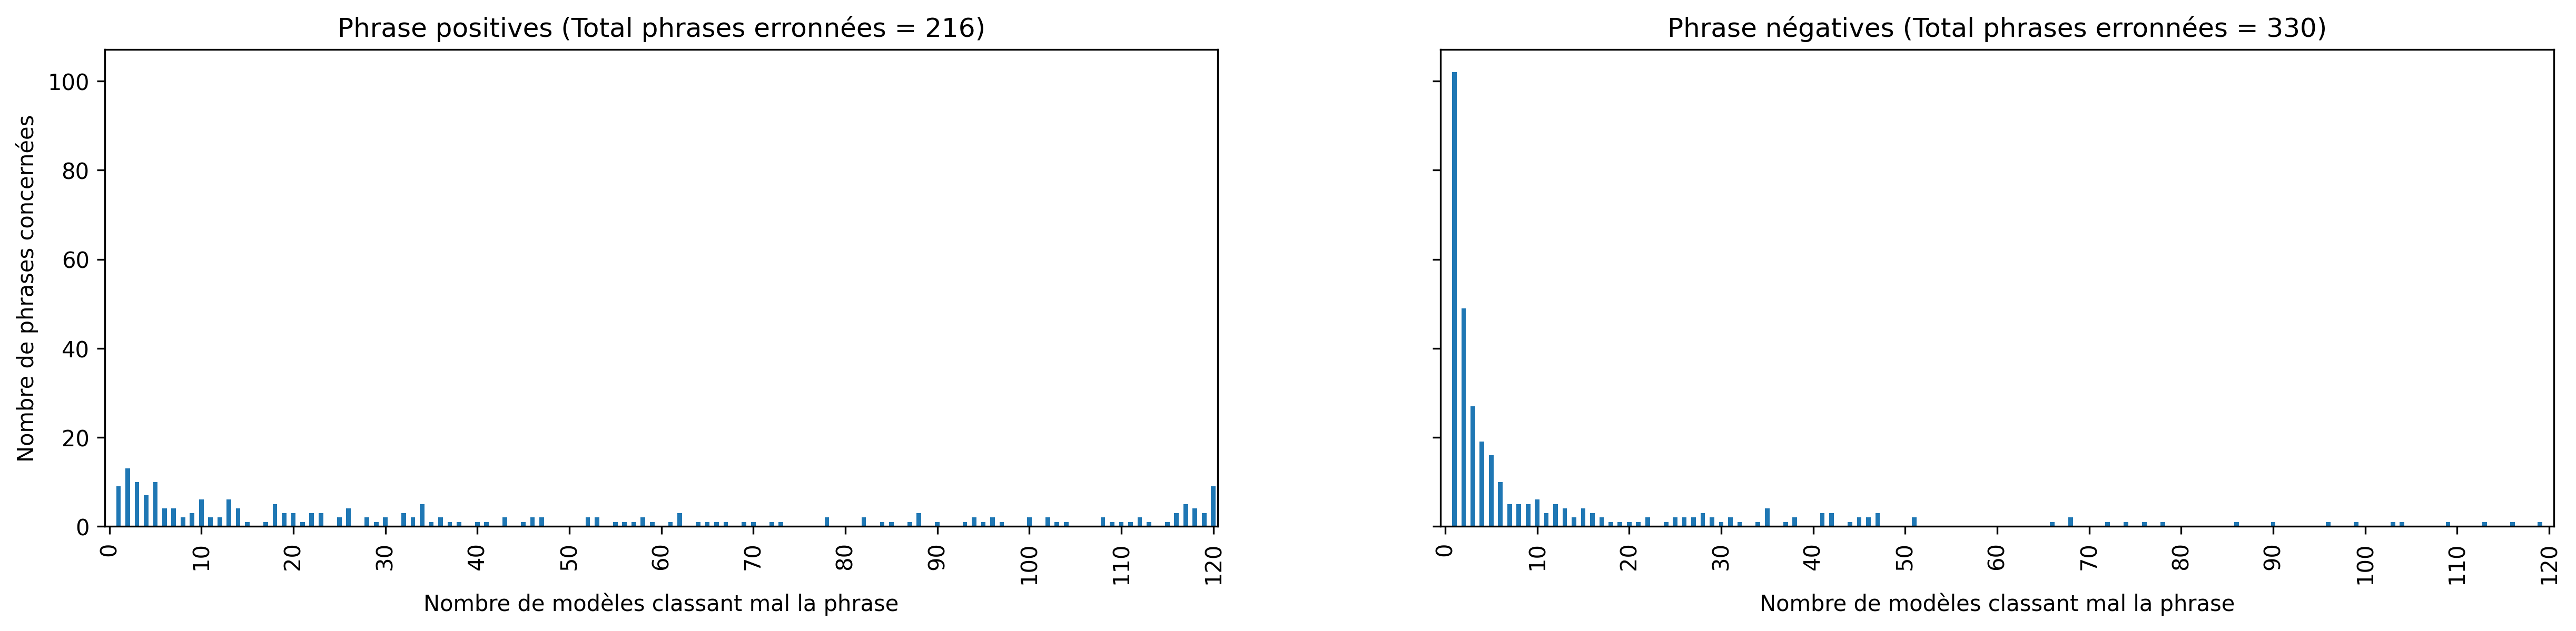
\includegraphics[width=\linewidth]{figures/commonErrors.png}
    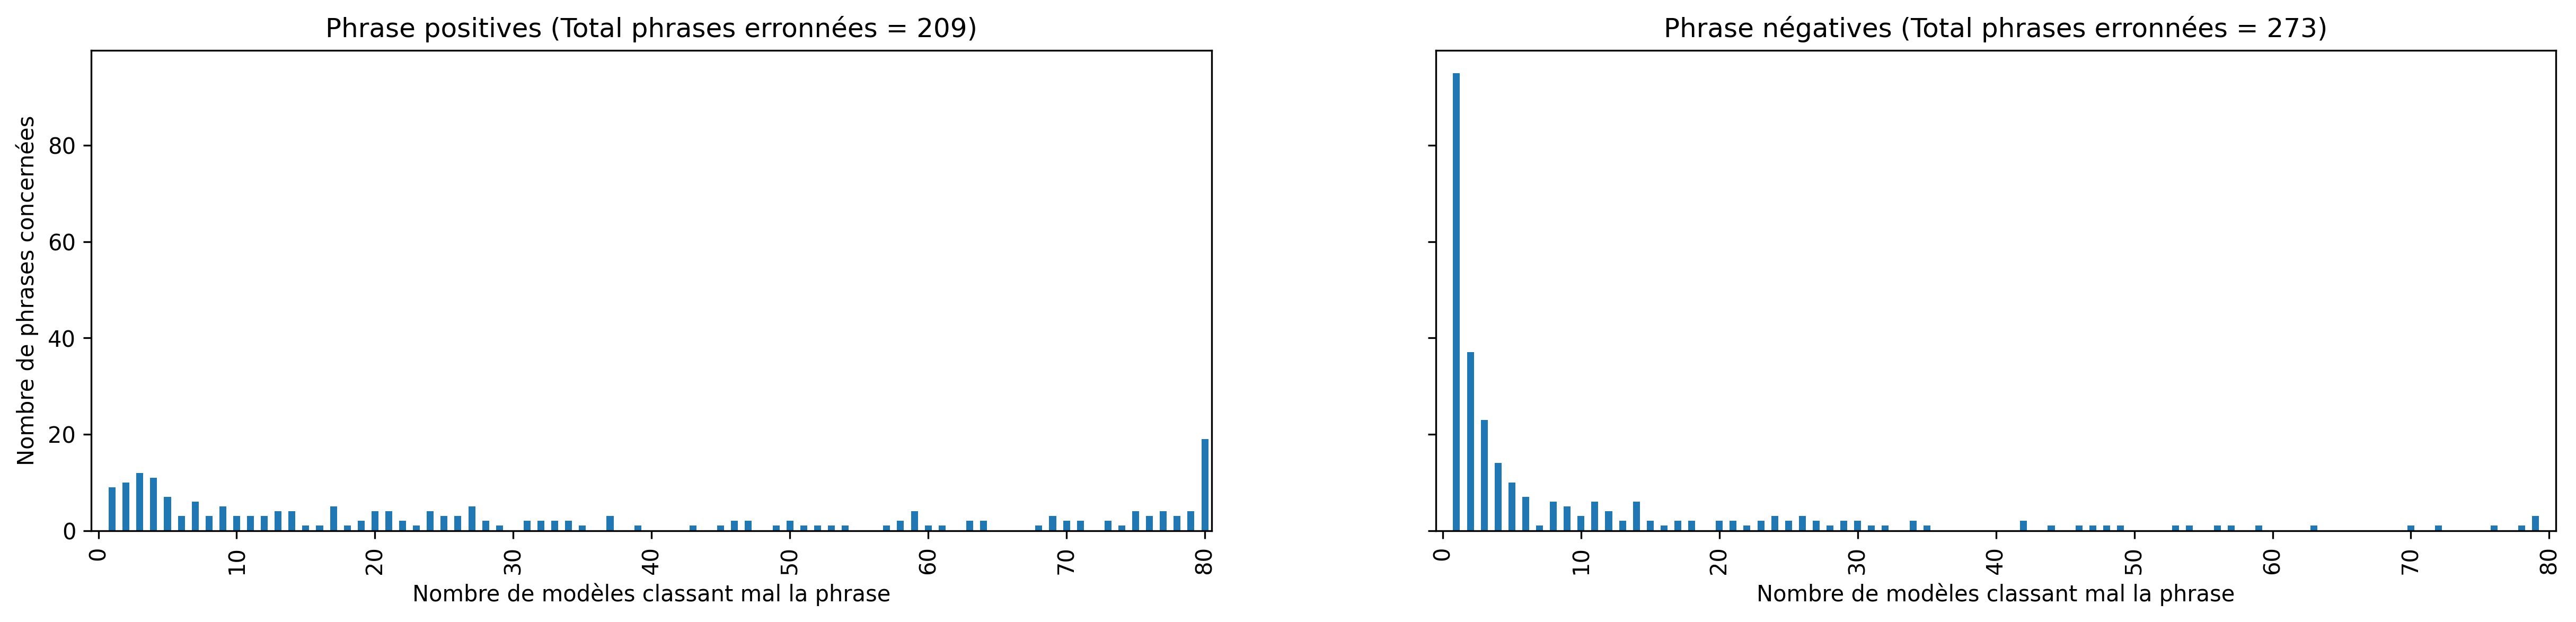
\includegraphics[width=\linewidth]{figures/commonErrorsNotEnriched.png}
    \caption{Répartition et décompte du nombre de modèles faisant des erreurs de classement. En haut à gauche, on lit: ``19 phrases positives sont mal classées par les 80 modèles pris en compte, tandis que plus de 80 phrases négatives ne sont mal classées que par un seul modèle parmi les 80 entraînements.''. En haut: les meilleurs modèles et les modèles sans enrichissements, en bas: les modèles sans enrichissements uniquement.}
    \label{fig:chap4:commonErrors}
\end{figure}

% Reprendre ICI

En figure \ref{fig:chap4:commonErrors}, on s'aperçoit d'une distribution des phrases négatives mal classées suivant la loi de puissance: elles sont nombreuses à être erronées chez un seul modèle et très rapidement très peu nombreuses ou inexistantes chez de nombreux modèles. Nous faisons l'hypothèse de la responsabilité croisée d'un artefact de l'entraînement du modèle, de la focalisation sur le score F1 de la catégorie positive et de l'extrême variété présente chez les exemples négatifs: ainsi qu'on l'a vu dans le cadre de l'attention, la définition de ce qui constitue un exemple ne portant pas d'isotopie sexuelle est compliquée pour le modèle, qui choisit la ponctuation comme ``indice'' d'absence. Il n'existe pas de phrase négative sur laquelle l'ensemble des modèles a produit une erreur de classement.

Au contraire, la distribution des phrases positives erronées est beaucoup plus équilibrée, avec un pic en départ de modèle, probablement dû à la part d'aléatoire des entraînements sus-cités, et un pic à la fin. Ce pic rejoint ce que l'on avait trouvé dans l'étude de l'attention: il existe des phrases qui sont potentiellement inclassables sans contexte pour le modèle. Aussi, nous proposons une lecture et catégorisation des neuf phrases communes aux cent vingt modèles entraînés, et des dix phrases supplémentaires qui ne sont pas reconnues spécifiquement par les modèles non enrichis. Trois catégories de phrases se trouvent en table \ref{tab:chap4:erreurscommunes}: des phrases presque impossibles à interpréter sexuellement hors contexte, des phrases difficiles, mais compréhensibles, et quelques exemples où la présence de la sexualité ne fait pas de doute.

\begin{table}[]
    \centering
    \small %
    \begin{tabularx}{\textwidth}{|r|r|X|X|}
    \toprule
    ID & Erreurs & Phrase & Source                                                                                                                                   \\ \midrule
    1     & 80               & \textit{iacere umorem in corpus de corpore ductum ;}  & Lucrèce, \textit{De Rerum Natura}, 3, 1056                                                                                              \\
    2     & 80               & \textit{"Dumque loquimur, sera sua sponte delapsa cecidit reclusaeque subito fores admiserunt intrantem.{[..."]}} & Pétrone, \textit{Satyricon}, 16                            \\
    3     & 80               & \textit{Quae, quia non liceat, non facit, illa facit!} & Ovide, \textit{Amours}, 3, 4, 4                                                                                       \\
    4     & 80               & \textit{A. Perii miser, quia pudicitiae huius vitium me hinc absente est additum.}  & Plaute, \textit{Amphitrion}, 809-810                                                             \\
    5     & 80               & \textit{ludite ut libet, et brevi liberos date.}  & Catulle, 61, 204-205                                                                                                \\
    6     & 80               & \textit{exigite ut sit et pater ipsius coetus, ne turpia ludant, ne faciant vicibus;}   & Juvénal, 7, 238-240                                                        \\
    7     & 80               & \textit{namque totius vobis frontem tabernae sopionibus scribam.}   & Catulle, 37, 9                                                                              \\
    8     & 80               & \textit{Quomodo tibi in actu illo ignominioso non veniebat in mentem habitus virginalis, processus in Ecclesiam inter virgineos choros ?} & Ps.-Ambroise, \textit{De lapsu virginis consecratae}, 6, 22         \\
    9     & 80               & \textit{Naidas antiqui Dryadasquehabuere Priapi, et quo tenta dei uena subiret, erat.}  & \textit{Priapées}, 33, 2                                                  \\
    10    & 80               & \textit{"Nube, precor, "dicet," cui te bona numina iungunt ;{[..."]}}    & Ovide, \textit{Héroïdes}, 20, 215                                                                            \\ \midrule
    11    & 120              & \textit{Lavacrum publicum in aedibus aulicis fecit, simul et Plautini populo exhibuit, ut ex eo condiciones bene vasatorum hominum colligeret.} & Histoire Auguste, \textit{Vie d'Héliogabale}, 8.6 \\
    12    & 120              & \textit{intactum ab omni crimine virginal, mortis deinde gloria liberae.} & Prudence, \textit{Passion de sainte Agnès}, 8                                                                       \\
    13    & 120              & \textit{Paratus miles arma non habui.} & Pétrone, \textit{Satyricon}, 130                                                                                        \\
    14    & 120              & \textit{tergum, colla, umeros, luteae Symplegadis antrum.} & Ausone, \textit{Épigrammes}, 104, 9                                                                                    \\
    15    & 120              & \textit{Vivite Concordes et nostrum discite munus.} & Claudien, \textit{Epithalame}, 141                                                                                              \\
    16    & 120              & \textit{Ego sic perire coepi.} & Pétrone, Satyricon, 11.51                                                                                                                   \\
    17    & 120              & \textit{Eccere, perii misera, quam tu mihi nunc navem narras ?} & Plaute, \textit{Les Ménechmes}, 402                                                                                 \\
    18    & 120              & \textit{post si quis vellet, te haud non velles dividi.} & Plaute, \textit{Aulularia}, 286                                                                                        \\ \bottomrule
    \end{tabularx}
    \caption{Phrases positives mal reconnues par l'ensemble des modèles. Les phrases mal reconnues par 120 modèles cumulés (de 11 à 18) sont aussi \textit{de facto} mal reconnues par les 80 modèles non enrichis  (1 à 10). Entre crochets se trouvent des guillemets fermants absents de la phrase traitée.}
    \label{tab:chap4:erreurscommunes}
\end{table}

\begin{quote}[\textit{Héroïdes}, 20, 215 ]{Ovide}
(10) ``Épouse, je t’en prie”, dira-t-elle, “celui à qui les volontés divines te joignent''
\end{quote}

\begin{quote}[\textit{Épithalame}, 141 ]{Claudien}
(15) ``Vivez en concorde et apprenez nos obligations.''
\end{quote}

\begin{quote}[\textit{Les Ménechmes}, 402]{Plaute}
(17) ``Voilà, malheureuse, je suis morte, de quelle péniche me parles-tu maintenant ?''
\end{quote}

Dans cette première catégorie des phrases impossibles, on retrouve les phrases 3, 13, 14 et 16 dont nous avions parlé précédemment. S'ajoutent à celles-ci trois phrases, la 10, la 15 et la 17. 

La phrase 15, issue de l'\textit{Epithalame} de Claudien, fait référence au \textit{munus}, le devoir conjugal. Mais, à côté de la notion de concorde, les sens plus généraux du mot (charge, obligation, office) liés à la fonction sociale ou étatique ne sauraient être exclus sans avoir accès au reste du texte. Si J. N. Adams la classe ainsi\footcite[p.~161]{adams}, c'est surtout grâce à son contexte: il est fait référence entre autres à \enquote{\textit{oscula mille}} (``mille baisers'', vers 142) et du passage du statut de femme à celui de mère (\enquote{Ainsi tu seras épouse, ainsi tu seras mère.}, vers 148\footnote{\enquote{\textit{sic uxor, sic mater eris.}}}): l'isotopie apparait à travers la récurrence des sèmes du mariage, de l'acte sexuel et de la reproduction, en dehors de l'extrait lui-même. 

Les deux autres posent des problèmes, y compris en contexte. Pour l'extrait d'Ovide, le doute autour du sens sexuel possible de \textit{iungo} ou de \textit{nubo} n'est pas levé par une lecture ``manuelle'' du texte, sachant que cette classification n'est pas issue du travail d'Adams, mais de celui du TLL, dont la mise en forme peut parfois porter à confusion\footnote{TLL, VII.2.65860ff}. Dans cette \textit{Héroïde 20}, les vers qui précèdent le 215 mettent en scène une mise à nu orchestré par le divin, mais ceux qui suivent font bien usage du lexique du mariage (``\textit{gener} (gendre)'' au vers 216, ``\textit{maritum} (mari)'' au vers 227). Il est difficile alors de pencher pour l'un ou pour l'autre des sens avec une assurance sans faille. Il est possible que le sous-entendu sexuel existe dans \textit{nubo}, mais il nous semble plus probable qu'il soit lointain et assez faible, comparé par exemple à la situation de \textit{munus} plus haut. Pour la dernière, issue des \textit{Ménechmes}, même Adams n'est pas tout à fait convaincu: ici, trois ouvrages, dont le \textit{Lewis and Short}, donnent le sens de sexe féminin à \textit{navem} (bateau, navire, traduit par péniche plus haut)\footcite[p~.89, note 1]{adams}. Il nous semble aussi difficile de soutenir cette analyse, peu de faisceaux en contexte nous permettant d'établir un double sens ici.

\starbreak

Six phrases nous semblent rentrer dans une catégorie ``compréhensible'': le contexte assure une confirmation du sens, mais il est possible de déceler des indices sans son aide.

\begin{quote}[\textit{De Rerum Natura}, 3, 1056]{Lucrèce}
    (1) \enquote{semer dans un corps le liquide tiré de son corps}
\end{quote}

\begin{quote}[61, 204-205]{Catulle}
     (5) \enquote{Jouez à votre gré et donnez-nous rapidement des enfants.}
\end{quote}

La première est celle de Lucrèce 1). \textit{Jacio} n'est pas utilisé seulement chez Lucrèce en ce sens de semer (le \textit{Gaffiot} donne Virgile, \textit{Géorgiques}, 1, 104). \textit{Humor} n'est pas particulièrement réservé aux fluides génitaux, mais il n'existe pas beaucoup de fluides censés passer d'un corps à un autre: on comprend alors facilement la difficulté de la machine à comprendre et savoir cela. De même, dans la phrase (5) de Catulle, l'idée du jeu (\textit{ludite}) et donc de /plaisir/ alliée à celle des enfants (\textit{liberos}) et de leur /production/ (\textit{date}, littéralement ``donnez'') ne laisse pas beaucoup d'espace au doute pour le lecteur qui s'attend à ce sujet. La relation syntaxique des termes semble nécessaire à comprendre l'isotopie: la relation cause-conséquence induite par la coordination jouer/donner, la relation verbe-objet (donner + enfants), et le modèle n'arrive pas, avec ses informations, à détecter celles-ci.


\begin{quote}[\textit{Amphitrion}, 809-810]{Plaute}
	(4) ``Amph. Malheureux, je suis mort, parce qu’en plus, alors que j’étais loin d’ici, la pudeur lui a fait défaut !''
\end{quote}

\begin{quote}[61, 204-205]{Catulle}
	(5) ``Jouez à votre gré et donnez-nous rapidement des enfants.''

\end{quote}

\begin{quote}[7, 238-240]{Juvénal}
	(6) ``Exigez qu’il soit aussi le père de leur troupe pour qu’ils ne jouent à des jeux honteux ni qu’ils ne le fassent à tour de rôle;''
\end{quote}

\begin{quote}[\textit{De lapsu virginis consecratae}, 6, 22]{Ps.-Ambroise}
	(8) ``Comment – pendant cette action dégradante – ne te venait pas à l’esprit l’habit virginal, la procession dans l’Église entre les choeurs virginaux ?''
\end{quote}

Pour les quatre autres phrases, des termes précis, communs à nos exemples, sont mentionnés: \textit{pudicitia} (pudeur), \textit{vitium} (vice), \textit{turpia}, et les différents dérivés de la virginité. Les jeux honteux, l'absence de pudeur, l'action dégradante (la perte de virginité) sont autant de faits qui ne laissent pas de doute. Il est intéressant de voir que ce sont les modèles ``classiques'', sans enrichissement, qui butent systématiquement sur ces phrases, là où les modèles enrichis arrivent à les prédire au moins quelques fois.

\starbreak

\begin{quote}[33, 2]{\textit{Priapées}}
    (9) Les Priapes d’autrefois avaient Naïades et Dryades, Et il y avait de quoi faire monter une veine tendue de dieu !
\end{quote}

\begin{quote}[Vie d'Héliogabale, 8, 6]{\textit{Histoire Auguste}}
    (11) Il construisit des bains publics dans les bâtiments du palais et, en même temps, il les ouvrit au peuple, afin de lister l'identité des hommes bien équipés.
\end{quote}
\begin{quote}[\textit{Passion de sainte Agnès}, 8]{\textit{Prudence}}
    (12) [Une double couronne fournit la tête de la martyre]: une virginité intacte de tout crime, ensuite la gloire d'une mort libre.
\end{quote}
\begin{quote}[\textit{Aulularia}, 286]{\textit{Plaute}}
    (18) Après, si quelqu’un voulait de toi, tu ne serais pas contre l'idée de te faire fendre!
\end{quote}

Ici, les termes spécifiques sont présents, y compris pour la (7), vue dans la section précédente, l'isotopie a le temps de se développer à chaque fois sans avoir besoin de recourir au contexte\footnote{On l'apporte simplement pour la phrase incomplète sinon de la \textit{passion de sainte Agnès}.}:
\begin{itemize}
    \item \textit{Priapi} (dieu connu pour son /érection/) est développé par \textit{tenta uena} (veine tendue, portant /phallus/ et /érection/) et \textit{subiret} (allez dessus, /chevauchement/);
    \item les \textit{lavacrum publicum} (bains, /nudité/) sont appuyés par le très clair \textit{vasatorum} (/gonade/);
    \item la notion de crime (\textit{crimen}) appliqué à la virginité (\textit{virginal}) et de l'absence de ``toucher'' (\textit{intactum});
    \item le /désir/ (\textit{vellet}) appliquée à une /personne/ (\textit{te}) et celle de fendre (\textit{dividi}), commune en latin, construite sur l'action /écarter/ + /insérer un objet dans la fente pour écarter plus/
\end{itemize}

Les cinq phrases ne laissent aucun doute et pourtant le modèle ne les reconnaît pas. Si nous avions vu que \textit{sopio} était un mot rare, la priapée ne partage pas cette rareté dans le corpus, rendant l'exemple comportant \textsc{Priapus} et \textsc{Vena} difficile à expliquer. Au contraire, \textsc{Vasatus} n'est présent que cinq fois, uniquement dans l'\textit{Histoire Auguste}, \textsc{divido} cinq fois, \textsc{virginal} quatre, expliquant peut-être l'incapacité des modèles à en intégrer le sens. Il est intéressant de voir que le modèle a su intégrer des phénomènes extra lexicaux, comme celui de la nuit donnée chez Ovide, mais n'est pas capable d'en détecter certains autres: \textsc{diuido} au passif + \textsc{tu} en sujet ne devraient pas laisser place au doute... 

Les modèles ne sont pas donc pas infaillibles, loin de là. Il est cependant intéressant de les voir buter sur les phrases où même la littérature scientifique ne se met pas d'accord (comme pour \textit{navem}). Les contraintes que nous avons imposées au modèle sont énormes vu le problème que nous avons cherché à résoudre, celui de la détection d'isotopies. Comme nous l'avons déjà vu dans la définition de ces dernières, elles se définissent par la récurrence de sèmes qui, ensemble, en ``créent un autre''. Or, nous avons toujours limité les extraits d'entraînement ou de détection à une phrase, produite par un éditeur, ou à un extrait encore plus réduit (comme l'exemple des Symplégades). Sans un contexte plus grand, le modèle ne peut finalement s'appuyer que sur des signaux très forts ou sur une récurrence de signaux bien identifiés, sur lesquels il s'est assez entraîné. Il reste à voir ce qu'il est possible de faire pour enrichir les modèles et améliorer la compréhension de ces phénomènes: gestion des relations syntaxiques (arbre de dépendance), des entités nommées et de leurs attributs -- notamment les fonctions divines --, des phénomènes de dérivation sans pour autant introduire le bruit qu'insère un outil comme \textit{FastText}. Par exemple, la relation entre \textit{coleus} (testicule) et \textit{coleatus} (pourvu de testicules), deux mots qui sont rares, pourrait aider à faire remonter le signal de chacun d'entre eux. % Mais cette question en appelle finalement une autre, qui est celle de la sélection des modèles et de leurs rôles dans l'analyse du latin.

% Parmi ces phrases, on reconnaît les phrases 3, 7, 13, 14, 16 qui ont été étudiées dans le cadre de l'analyse de l'attention. On reconnaît les catégories ici des exemples précédemment reçus: de nombreuses phrases ont un sens particulièrement compliqué à comprendre hors contexte.
%Erreurs les plus fréquentes: Quels tags ? Quels mots ?

%Classification des types d’erreurs

%	Sur-apprentissage (Martial == Sexe)

%	Sous-apprentissage (Termes de la guerre =? Sexe)

\section{Quel modèle choisir ?}

\begin{quote}[\enquote{\textit{‘Improving ratings’: audit in the British University system}}]{Marilyn Strathern}
    Quand une mesure devient une cible, elle cesse d'être une bonne mesure.\footnote{\textit{\enquote{When a measure becomes a target, it ceases to be a good measure.}} \textcite{strathern_improving_1997}}
\end{quote}

Bien qu'issue d'un travail en dehors de nos disciplines, la citation de M. Strathern résonne avec des inquiétudes, des remarques, des discussions du monde des humanités numériques quand elles font face à cette nouvelle approche computationnelle qu’ on lui applique. Une première réponse au titre ici pourrait être de dire: utilisons le meilleur modèle, à chaque fois. Mais elle ne nous semble pas adaptée, non seulement car nous avons finalement vu que les meilleurs scores pouvaient cacher une forme de triche -- ou surentraînement -- des réseaux, mais que, le corpus étant si petit, la variation des scores était assez grande.

Il nous semble que le cas le plus commun d'usage de cet outil serait de partir d'un jeu d'échantillons ne comprenant que des données obtenues par recherche lexicale. Il serait ainsi facile de compiler un premier corpus de couleurs en latin en n'utilisant que quelques couleurs bien identifiées. Sur la version d'\textit{Alpheios} de \textit{Blacklab}\footnote{\url{https://blacklab.alpheios.net}}, une version ``pauvre'' de notre corpus culminant à 16M de tokens, une recherche comprenant 15 lemmes adjectifs de couleurs retrouvent ainsi 5~870 occurrences\footnote{Requête CQL: {[(lemma = "albus|argenteus|aureus|brunus|caeruleus|caerulus|cupreus|flauus|luteus|niger|purpureus\\|rauus|ruber|russus|uiridis") \& pos = "ADJqua" ]}}, soit plus du triple du corpus d'Adams. Pour d'autres sujets, ce corpus serait peut-être plus petit (\textit{e.g.} le corpus de la petite enfance, de l'allaitement, des meutes, etc.). D'après les résultats du modèle sur le corpus Non-Métaphores, les modèles HAN, enrichis ou non, sont adaptés à ce genre de corpus d'entraînement. Par ailleurs, dans une approche de filtrage humain et d'interprétation des textes, les modèles HAN offrent, avec leur mécanisme d'attention, une compréhensibilité supérieure, car ils permettent de trouver rapidement ce qui importe pour le modèle dans la phrase, et de détecter potentiellement les écarts entre les attentes du philologue ou lexicographe et celles du modèle. 

Reste alors la question de l'architecture en elle-même autour de l'encodeur HAN. L'usage d'enrichissement est dépendant de la relative dilution de la ``thématique'' et des exemples originaux dans le corpus d'entraînement, mais cette approche insère le risque de surspécialisation, qui, dans une logique de recherche de données et non d'obtention du meilleur score, est à éviter. Pour le reste de l'architecture, les modèles HAN obtiennent de meilleurs résultats avec BERT pour de très petits corpus, alors que Word2Vec comme projection marche correctement ailleurs. Nous avons parlé de BERT plus tôt, et ses résultats ont finalement été décevants, vu le coût en production et en prédiction: ne pas l'utiliser ne serait pas une erreur.

Quoiqu'il en soit, cet outil s'intègrera au mieux dans un processus itératif d'entraînement~-~correction des prédictions~-~entraînement pour inclure, peu à peu, les isotopies correctement détectées et augmenter le set de données, et remettre au centre de la chaîne de recherche les spécialistes du domaine.